\documentclass{article}
\usepackage{amsmath}
\usepackage{amssymb}
\usepackage{amsthm}
\usepackage{breqn}
\usepackage{enumitem}
\usepackage{graphicx}
\usepackage{hyperref}
\usepackage{mathtools}
\usepackage{pgfplots}
\usepackage{subcaption}
\usepackage{xcolor}
\usepackage[margin=4cm]{geometry}

\usetikzlibrary{calc}
\pgfplotsset{compat=newest}

\title{\textbf{Hessian Eigenspectra of Nonlinear Neural Networks}}
\author{Sabri Meyer \bigskip \\ \bigskip \textbf{Master Thesis in Mathematics} \\ \emph{Supervision:} \\ \emph{Prof. Dr. Aurelien Lucchi, Prof. Dr. Jiří Černý}}
\date{\emph{University of Basel} \\ \emph{September 15th, 2023}}

\begin{document}
\numberwithin{equation}{section}

\newtheorem{common}{Common}[subsection]
\newtheorem{definition}[common]{Definition}
\newtheorem{proposition}[common]{Proposition}
\newtheorem{lemma}[common]{Lemma}
\newtheorem{theorem}[common]{Theorem}
\newtheorem{corollary}[common]{Corollary}
\newtheorem{assumption}[common]{Assumption}

\maketitle
\thispagestyle{empty}

\begin{abstract}
In this master's thesis, we investigate the limiting Hessian eigenspectrum of neural network models featuring nonlinear activation functions. Our approach relies on the Bai-Silverstein analysis, exploiting concentration inequalities for specific quadratic forms for large random matrices. By relating these forms to the trace of the Hessian resolvent matrix, and thus its limiting Stieltjes transform, we establish a self-consistent equation for the latter. Solving this equation, we apply the Stieltjes inversion formula to reconstruct the limiting spectral density used for numerical simulations\footnote{\href{https://github.com/sabrimeyer/master-thesis}{https://github.com/sabrimeyer/master-thesis}}. This information sheds light on the loss landscape, e.g. the Hessian condition at random initialization of trainable parameters, and also during training.
\end{abstract}

\newpage
\tableofcontents

\newpage

\section{Introduction}
Neural networks have emerged as a powerful tool for tackling complex problems across various domains, including pattern recognition, natural language processing, and generative AI. Despite their widespread success, understanding the intricate workings of neural networks, particularly deep neural networks, remains a formidable challenge. A critical aspect of this challenge lies in studying the properties of the loss landscapes in parameter space. The parameters, often represented as weights and biases, define a network's behavior and are adjusted during learning to minimize the loss function. The dimensionality of this parameter space corresponds to the total number of parameters in the model, making it highly complex in practical applications. Effectively exploring and navigating this parameter space is essential for optimizing model performance, and understanding its geometry is a central focus in the field of deep learning \cite{pennington,orvieto}.
\bigskip
\par
The Hessian matrix of the loss function, within the expansive parameter space of neural networks, plays a pivotal role in characterizing the local curvature and geometry of the loss landscape. By examining its eigenvalues, valuable insights into the landscape's shape and regions of fast or slow convergence during optimization can be gained. Therefore, a comprehensive analysis of the Hessian eigenspectrum not only enhances our understanding of neural network behavior but also contributes to the development of more efficient and stable training procedures for deep learning models \cite{Liao, wu, sankar, kawaguchi}.
\par
Before studying general deep neural networks, it is beneficial to develop a solid understanding of shallow neural networks \cite{pennington2, piccolo, soltanolkotabi, arjevani}. When studying these networks, the Hessian exhibits a concrete structure which can be analyzed using direct means such as probability theory, and random matrix theory \cite{couillet, benigni, louart, hachem, vershynin, tao}. This eventually lead to the Bai-Silverstein approach that we employ in this thesis \cite{bai}.
\bigskip
\par
Determining the spectral distribution of a random Hessian matrix, constructed from randomly sampled data (or depending on randomly initialized weights), poses a challenging task that requires advanced mathematical techniques. The Stieltjes transform, a powerful mathematical tool, proves useful in characterizing the spectral measure and distribution of the Hessian matrix \cite{couillet}. By employing concentration inequalities for quadratic forms for large random matrices, we can derive a fixed-point equation for the Stieltjes transform \cite{couillet, rudelson, louart}. Solving this equation finally provides an explicit formula for the spectral distribution of the underlying Hessian. In this context, we consider the limiting Stieltjes transform, where the number of data entries and their features tend towards infinity. This approach yields a continuous spectral density rather than an empirical spectral distribution.
\bigskip
\par
The goal of this work is to contribute fresh perspectives to the eigenspectrum of shallow neural networks with nonlinear activations. More precisely, we aim to employ the Bai-Silverstein method on a single-layer network and subsequently broaden our examination to the two-layer scenario. In this process, we discover the advantages and limitations of this approach and compare our results with other, already established ones. Numerical experiments are conducted to verify our theoretical findings and grant intuitive interpretations for further discussions. For an overview of our outcomes, we refer to the conclusion at the end of this thesis.
\par








\section{Related Works}
In order to derive a self-consistent equation for the limiting Stieltjes transform for the corresponding Hessian, we rely on the methodology proposed by Bai and Silverstein \cite{bai}, which exploits rank-1 perturbations in the structure of the Hessian, applies the Sherman-Morrison-Woodbury formula and uses concentration arguments. Since we focus on the asymptotic case, where the number of data points and their features both tend to infinity $n,d\to\infty$, the concept of deterministic equivalents of random matrices plays a central role \cite{couillet}. This kind of Bai-Silverstein analysis is conducted by Liao et al. \cite{Liao}, who study the limiting spectral distribution of the Hessian at random initialization. Their Theorem 1 is comparable with our first main result, Theorem \ref{thm:mainresult-1}. Additionally, Liao et al. consider spiked models of the Hessian, where isolated eigenvalues and multiple bulks of the spectral distribution start to appear.
\bigskip
\par
The works of Mannelli et al. \cite{mannelli} analyses the limiting spectral distribution of the phase retrieval model, which coincides with our nonlinear regression model for a quadratic activation $\phi(x)=x^2$. Using gradient descent methods, they study the time-evolution of the spectral density of the Hessian for different values of the sample-ratio $\alpha:=\lim_{n,d\to\infty}n/d$. Moreover, by using methods from statistical physics, they provide critical values for $\alpha$ for which BBP phase transitions occur, where eigenvalues leave the bulk of the spectral density.
\bigskip
\par
In deep learning, when studying the Hessian eigenspectrum of neural networks with multiple layers, it is common practice to separately study the spectrum of each individual layer-wise Hessian \cite{wu, bahamou, sankar}. The full Hessian is then a block matrix, where each diagonal block represents the layer-wise Hessian of the corresponding layer \cite{kawaguchi}. We are particularly interested in studying the Hessian eigenspectrum of shallow neural networks (i.e. networks with one hidden layer) with general activation functions. For ReLU-activations, \cite{pennington} propose $\mathcal{R}$-transform methods applied on the Gauss-Newton decomposition $\mathcal{H}=H_0+H_1$ of the Hessian to derive a fixed-point equation for the limiting Stieltjes transform. However, their approach requires free independence of $H_0$ and $H_1$, which they only justify empirically. In another study, Pennington et al. \cite{pennington2} relied on the method of moments to find a fixed-point equation for the Stieltjes transform of the positive semi-definite part $H_0$.
\par
A very interesting result is the comparison with \cite{benigni, piccolo}, who study the limiting spectral distribution of the modified covariance matrix $H_2:=\phi(WX)^\top\phi(WX)/n$ for some general activation $\phi$ ($n$ being the number of samples), where $W$ and $X$ denote the weight- and the data-matrix, respectively. This matrix coincides exactly with the second-layer Hessian $H_2$ arising in our shallow neural network model. They use the method of moments to derive a fixed-point equation for the limiting Stieltjes transform (also see Theorem \ref{thm:peche}).
\bigskip
\par
For studies in the non-asymptotic regime, we refer to the paper by \cite{soltanolkotabi} who show global regularity properties of the loss landscape in the case of the quadratic activation function $\phi(x)=x^2$. The paper also takes into account the training of the neural network with general activations $\phi$, providing convergence rates of the loss function. Another reference is the study of Arjevani et al. \cite{arjevani}, who focus specifically on finding the eigenvalues of the Hessian for a shallow ReLU-network.


\section{Motivation}
Let us begin with a simple model; the linear regression model. In order to formulate the optimization problem, we need to introduce a the loss function. Afterwards, we will derive the structure of the underlying Hessian. The Hessian coincides with a scaled covariance matrix, and it is already known that the spectrum of such a random matrix follows the Marchenko-Pastur law.
\subsection{Hessian of the Linear Regression Model}
We consider the optimization problem that involves the least square objective, expressed by the loss function
\begin{equation}
\mathcal{L}(w):=\frac{1}{2n}\sum_{i=1}^n(w^\top x_i-y_i)^2,\label{eq:loss-1}
\end{equation}
where we aim to train the weight-vector $w\in\mathbb{R}^d$ using random labeled data $\{(x_i,y_i)\}_{i=1}^n$ with $x_i\in\mathbb{R}^d$ and $y_i\in\mathbb{R}$. Alternatively, we can represent the loss function as
\begin{equation}
\mathcal{L}(w)=\frac{1}{2n}\|X^\top w-y\|^2,
\end{equation}
where the random matrix $X:=[x_1,\dots,x_n]\in\mathbb{R}^{d\times n}$ and the random vector $y:=[y_1,\dots,y_n]^T\in\mathbb{R}^n$ are introduced. The global minimizer is denoted by
\begin{equation}
w^*:=\arg\min_{w\in\mathbb{R}^d}\mathcal{L}(w).\end{equation}
\par
To analyze the properties of the loss landscape, we study the Hessian $\mathcal{H}$ given by
\begin{equation}
\mathcal{H}_{ij}:=(\nabla_w^2\mathcal{L})_{ij}:=\frac{\partial\mathcal{L}}{\partial w_i\partial w_j}.
\end{equation}
\smallskip
\\
\begin{proposition}\label{thm:covariance}
The Hessian of the loss (\ref{eq:loss-1}) equals
$$\mathcal{H}(w)=\frac{1}{n}X X^\top.$$
\end{proposition}
\smallskip
\noindent
\emph{Proof.} We shall employ the convenient notation $\nabla_x f(x)$ to represent the Jacobian matrix of a vector-valued function $f(x)$. The first gradient is computed using the chain rule,
\begin{align}
\nabla_w\mathcal{L}(w) &= \frac{1}{2n}\nabla_w(\|X^\top w-y\|^2) = \frac{1}{2n}(2(X^\top w-y)^\top\nabla_w(X^\top w-y)) \notag
\\&= \frac{1}{n}(X^\top w-y)^\top X^\top = \frac{1}{n}X(X^\top w-y).
\end{align}
\par
Note that we made use of the elementary fact that $\nabla_x(|x|^2)=2x$ for any vector $x$, and the symmetry of the inner product in the last step. As a result,
\begin{align}
\mathcal{H}(w) &= \nabla_w^2\mathcal{L}(w) = \nabla_w(\nabla_w\mathcal{L}(w)) = \frac{1}{n}\nabla_w(X X^\top w-X y))=\frac{1}{n}X X^\top,
\end{align}
since $\nabla_w(X y)=0$.
\qed
\bigskip
\par
Observe that the Hessian $\mathcal{H}(w)=\mathcal{H}$ is independent of the weights $w$. Moreover, the form of the Hessian immediately implies that $\mathcal{H}$ is positive semi-definite. Indeed, for any $v\in\mathbb{R}^d$ we can see that
\begin{equation}
v^\top\mathcal{H}v=\frac{1}{n}v^\top X X^\top v=\frac{1}{n}(X^\top v)^\top(X^\top v)=\frac{1}{n}\|X^\top v\|^2\geq0.
\end{equation}
Geometrically this means that the loss $\mathcal{L}$ is convex. In particular, the global minimum is uniquely determined and easily attained when using optimization algorithms.

\subsection{Applying the Marchenko-Pastur Law}
As mentioned previously, we are able to describe the spectrum of the Hessian in Proposition \ref{thm:covariance} above by using the Marchenko-Pastur Law.
\begin{proposition}\label{thm:MP}
Let $X\in\mathbb{R}^{d\times n}$ is a random data-matrix with i.i.d. entries $X_{ij}$ such that $\mathbb{E}[X_{ij}]=0$, $\mathbb{E}[X_{ij}^2]=1$ and $\mathbb{E}[|X_{ij}|^8]<\infty$. Let $Y_n:=\frac{1}{n}X X^\top$, and denote its eigenvalues with $\lambda_1\leq\dots\leq\lambda_d$. Assume that
$$\mu_d(A):=\frac{1}{d}\#\{\lambda_j\in A\},\quad A\in\mathcal{B}(\mathbb{R}),$$
converges to some measure $\mu$ in distribution as $n,d\to\infty$, where $d/n\to \frac{1}{\alpha}\in(1,\infty)$. Then, the edges of the support of $\mu$ are given by
$$\lambda_\pm=\left(1\pm\sqrt{\frac{1}{\alpha}}\right)^2.$$
\end{proposition}
\smallskip
\noindent
\emph{Proof.} We refer to the discussion following the proof of Theorem \ref{thm:MP-stieltjes}.
\qed
\bigskip
\par
By Proposition \ref{thm:covariance} we know that the Hessian is of the form
\begin{equation}
\mathcal{H}(w)=\frac{1}{n}X X^\top.
\end{equation}
Therefore, we may directly apply Proposition \ref{thm:MP} to the matrix $Y_n:=\mathcal{H}(w)$ above, and the following statement follows.
\bigskip
\begin{corollary}\label{thm:lambda_pm}
Let $\mathcal{H}$ be the Hessian of the loss (\ref{eq:loss-1}), and assume that the data points ${(x_i)}_{i=1}^n$ are realizations of some probability distribution s.t. $X\in\mathbb{R}^{d\times n}$ has zero mean entries with unit variance and finite eighth-order moment. Let $d/n\to\frac{1}{\alpha}\in(1,\infty)$ as $n,d\to\infty$. Then, the smallest and largest eigenvalues of $\mathcal{H}$, in the limit $n,d\to\infty$, are almost surely given by
$$\lambda_\pm(\alpha)=\left(1\pm\sqrt{\frac{1}{\alpha}}\right)^2.$$
\end{corollary}


\subsection{Implications for the Hessian Condition}
The sample ratio, i.e. the ratio between the data samples $n$ and the number of data features $d$ is a particularly interesting quantity in our optimization problem, as it has a significant influence on the condition number of the Hessian. It is given by
\begin{equation}
\alpha:=\lim_{d,n\to\infty}\frac{n}{d}.
\end{equation}
Based on Corollary \ref{thm:lambda_pm}, we deduce that the Hessian of the loss function (\ref{eq:loss-1}) exhibits a condition number denoted by
\begin{equation}
\kappa(\alpha):=\left |\frac{\lambda_+(\alpha)}{\lambda_-(\alpha)}\right |=\left(\frac{1+\sqrt{\frac{1}{\alpha}}}{1-\sqrt{\frac{1}{\alpha}}}\right)^2=\left(\frac{1+\sqrt{\alpha}}{1-\sqrt{\alpha}}\right)^2\label{eq:kappa-MP}.
\end{equation}
\par
It is known that the performance of gradient descent algorithms enhances as the condition number $\kappa(\alpha)$ approaches 1 (refer to Appendix \ref{sec:appendix_optimization}). This implies that gradient descent becomes more manageable when $\alpha$ is sufficiently large (e.g., by increasing $n$ while keeping $d$ fixed). In other words, increasing the number of data points relative to the feature dimension, improves the learning capacity of the model (refer to Figure \ref{fig:condition}). Increasing $\alpha$ to a large extent is referred to as over-parametrization \cite{soltanolkotabi, mannelli}.
\par
\begin{figure}[!htb]
\centering
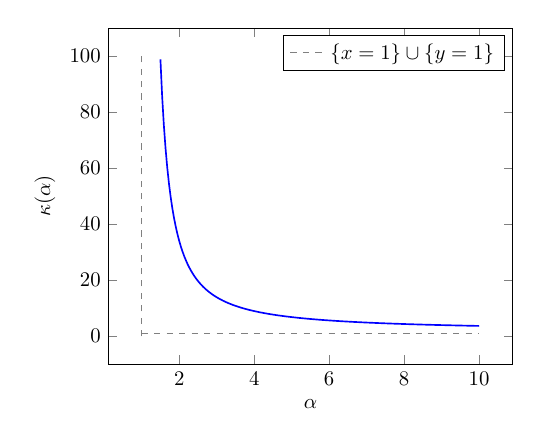
\begin{tikzpicture}[scale=0.75]
            \begin{axis}[ylabel=$\kappa(\alpha)$, xlabel=$\alpha$, restrict y to domain = 0:100]
                \addplot[samples=200, domain=1:10, blue, thick] {((1+sqrt(x))/(1-sqrt(x)))^2};
                \addplot[domain=1:10, gray, dashed] {1};
                \addplot[domain=0:2, gray, dashed] coordinates {(1,0) (1,100)};
                \legend{,$\{x=1\}\cup\{y=1\}$}
            \end{axis}
\end{tikzpicture}
\captionof{figure}{Asymptotic behaviour of $\kappa(\alpha)$}\label{fig:condition}
\end{figure}


\newpage
\section{Interlude: Illustrating Neural Networks}
This section aims to provide the mathematical definitions essential for understanding general neural networks. By additionally including visual representations of these networks, we try to facilitate the intuitive comprehension of the mathematical notation.

\subsection{Definition of Neural Networks}
In general, a (feed-forward) neural network can be mathematically defined as follows:
\begin{definition}[Neural Network]\label{def:NN}
A neural network with $L\in\mathbb{N}$ layers is a function $f^{(L)}_\theta:\mathbb{R}^d\to\mathbb{R}^m$ recursively defined as the composition
$$f_\theta^{(l)}(x):=\phi^{(l)}(W^{(l)}f_\theta^{(l-1)}(x)+b^{(l)}),\quad f_\theta^{(0)}(x):=x\quad\text{for}\quad l=1,\dots,L,$$
where $x\in\mathbb{R}^d$ is the input vector, $f_\theta^{(L)}(x)\in\mathbb{R}^m$ the output vector and $\phi^{(l)}$ the activation function in the $l$-th layer, which is applied point-wise. Here $\theta$ represents a set of (trainable) parameters
$W^{(l)}$ and $b^{(l)}$ being the weight matrix and the bias vector in the $l$-th layer, respectively.
\par
The weight matrix $W^{(l)}$ of the $l$-th layer is of the following form: For each $l=1,\dots,L$ let $d_l$ denote the number of nodes in the $l$-th layer. All weight connections from layer $l-1$ to the $l$-th layer are compiled in the matrix
\begin{equation*}
W^{(l)}:=\begin{bmatrix} \uparrow & \uparrow & & \uparrow \\ {W_1^{(l)}} & {W_2^{(l)}} & \cdots & {W_{d_{l-1}}^{(l)}} \\ \downarrow & \downarrow & & \downarrow \end{bmatrix}\in\mathbb{R}^{d_{l}\times d_{l-1}}.
\end{equation*}
\end{definition}
\bigskip
\indent
For each $k=1,\dots,d_{l-1}$, the column vector $W_k^{(l)}$ only consists of the weights originating from the $k$-th node $(f_\theta^{(l-1)}(x))_k$ in layer $l-1$, connecting to all the nodes in layer $l$. In this notation, this means that $f_\theta^{(l-1)}(x)\in\mathbb{R}^{d_{l-1}}$ and $b^{(l)}\in\mathbb{R}^{d_{l}}$. Also note that $d_0=d$ and $d_L=m$.
\bigskip
\\
\begin{figure}[!htb]
\centering
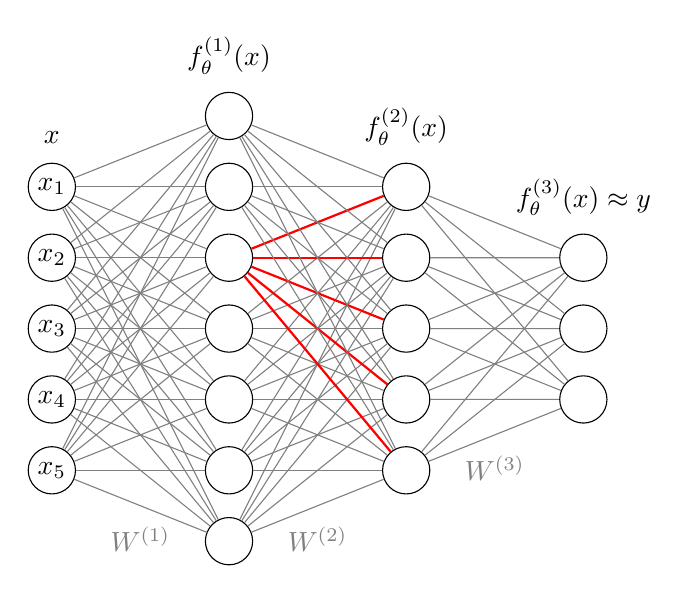
\begin{tikzpicture}[scale=0.75]

% Input layer nodes
\foreach \i in {1,2,3,4,5}
\node[circle, draw=black, minimum size=6mm] (I\i) at (0,\i*1.2-3.6) {};

% Hidden layer 1 nodes
\foreach \i in {1,2,3,4,5,6,7}
\node[circle, draw=black, minimum size=6mm] (H1\i) at (3,\i*1.2-4.8) {};

% Hidden layer 2 nodes
\foreach \i in {1,2,3,4,5}
\node[circle, draw=black, minimum size=6mm] (H2\i) at (6,\i*1.2-3.6) {};

% Output layer nodes
\foreach \i in {1,2,3}
\node[circle, draw=black, minimum size=6mm] (O\i) at (9,\i*1.2-2.4) {};

% Input layer to hidden layer 1 connections (with first edges in red)
\foreach \i in {1,2,3,4,5}
\foreach \j in {1,2,3,4,5,6,7}
\draw[gray] (I\i) -- (H1\j);

% Hidden layer 1 to hidden layer 2 connections (with first edges in red)
\foreach \i in {1,2,3,4,5,6,7}{
\foreach \j in {1,2,3,4,5}{
\ifnum\i=5
\draw[red, thick] (H1\i) -- (H2\j);
\else
\draw[gray] (H1\i) -- (H2\j);
\fi
}}

% Hidden layer 2 to output layer connections
\foreach \i in {1,2,3,4,5}
\foreach \j in {1,2,3}
\draw[gray] (H2\i) -- (O\j);

% Labels
\foreach \i/\name in {1/$x_5$, 2/$x_4$, 3/$x_3$, 4/$x_2$, 5/$x_1$}
\node (I\i) at (0,\i*1.2-3.6) {\name};
\node[align=center, above=2cm] at (I3.north) {$x$};
\node[align=center, above=2.8cm] at (H14.north) {$f_\theta^{(1)}(x)$};
\node[align=center, above=0.1cm] at (H25.north) {$f_\theta^{(2)}(x)$};
\node[align=center, above=1cm] at (O2.north) {$f_\theta^{(3)}(x)\approx y$};
\node[align=center, above=-0.7cm, gray] at ($(I1)!0.5!(H11)$) {$W^{(1)}$};
\node[align=center, above=-0.7cm, gray] at ($(H11)!0.5!(H21)$) {$W^{(2)}$};
\node[align=center, above=-0.7cm, gray] at ($(H21)!0.5!(O1)$) {$W^{(3)}$};

\end{tikzpicture}[h!]
\captionof{figure}{Example of a three-layer ($L=3$) neural network. The input vector $x\in\mathbb{R}^5$ is represented as the first column of nodes. The first and second hidden layers ($l=1$ and $l=2$) then output the column vectors $f_\theta^{(1)}(x)\in\mathbb{R}^7$ and $f_\theta^{(2)}(x)\in\mathbb{R}^5$, respectively. Finally, the result of the entire network is given by the output vector $f_\theta^{(3)}(x)\in\mathbb{R}^3$. Highlighted in red: The column $W_3^{(2)}$ of the matrix $W^{(2)}$ containing all weight entries adjacent to the node $(f_\theta^{(1)}(x))_3$, i.e. the third component of $f_\theta^{(1)}(x)$.}\label{fig:NN}
\end{figure}
\par
Definition \ref{def:NN} above tells us that $f_\theta^{(L)}$ is a composition of $L$ activations, in which each pre-activated output $W^{(l)}f_\theta^{(l-1)}(x)+b^{(l)}$ represents a linear transformation of the previous, activated output $f_\theta^{(l-1)}(x)$. The consequent activation $f_\theta^{(l)}(x)$ is then obtained simply by applying an element-wise non-linearity $\phi^{(l)}$. Refer to Figure \ref{fig:NN} for an illustration of such a neural network.
\par
It is a common model assumption that all activation functions are identical, i.e., $\phi^{(1)},\ldots,\phi^{(L)}\equiv\phi$. Naturally, this simplifies the network architecture.

\subsection{Loss Function of Neural Networks}
When presented with a collection of labeled data, we may introduce an appropriate loss function $\mathcal{L}$ to formalize the optimization problem of the neural network. The general definition of a loss function is found below.
\bigskip
\begin{definition}[Loss Function]
Let $\{(x_i,y_i)\}_{i=1}^n$, with $x_i\in\mathbb{R}^d$ and $y_i\in\mathbb{R}^m$, be the labeled data for our neural network $f_\theta^{(L)}$ as in Definition 2.1. The loss function is then defined as
$$\mathcal{L}(\theta):=\frac{1}{n}\sum_{i=1}^n\ell(y_i,f_\theta^{(L)}(x_i))$$
for some suitable choice of a scalar loss $\ell:\mathbb{R}^m\times\mathbb{R}^m\to\mathbb{R}_{\geq0}$. The optimization problem of the neural network can be formulated as finding the optimal parameter $\theta^*$ that minimizes the loss function $\mathcal{L}(\theta)$,
$$\theta^*:=\arg\min_{\theta}\mathcal{L}(\theta).$$
\end{definition}
\smallskip
\par
Indeed, during the optimization process over $\theta$, we aim to obtain the optimal choices for weights $W^{(l)}$ and biases $b^{(l)}$ that minimize the loss function $\mathcal{L}(\theta)\geq 0$. This procedure is commonly referred to as ''training the neural network''. By iteratively adjusting the parameters through techniques such as gradient descent, the network learns to make predictions and improve its performance on the given task.
\par
In this document, our particular focus lies on the quadratic loss function
\begin{equation}
\ell(y_i,f_\theta^{(L)}(x_i))=\frac{1}{2}\|f_\theta^{(L)}(x_i)-y_i\|^2.
\end{equation}
Other commonly used choices for the loss function $\ell$ include the mean absolute error loss, or cross-entropy losses. These alternative loss functions serve various purposes and are often employed based on the specific requirements of the neural network task at hand.

\subsection{Hessian of Neural Network Loss Functions}
We are particularly interested in studying the Hessian matrix $\mathcal{H}$ of the loss function $\mathcal{L}$ because it provides information about the curvature of the loss landscape. To facilitate its computation, it is convenient to vectorize the weights $W^{(l)}$ using the bijection
\begin{align}W^{(l)}=\begin{bmatrix} \uparrow & & \uparrow \\ {W_1^{(l)}} & \cdots & {W_{d_{l-1}}^{(l)}} \\ \downarrow & & \downarrow \end{bmatrix}\mapsto\quad&(\leftarrow {W_1^{(l)}}^\top\rightarrow\,,\,\dots\,,\,\leftarrow{W_{d_{l-1}}^{(l)}}^\top\rightarrow)^\top
\\ &\equiv (W^{(l)}_{1,1},\dots,W^{(l)}_{d_l,1},\dots,W^{(l)}_{1,d_{l-1}},\dots,W^{(l)}_{d_l,d_{l-1}})^\top \notag
\\ &=\operatorname{vec}(W^{(l)})=:\vec{w}_l \notag
\end{align}
for each $l=1,\dots,L$. In this case, the Hessian is given by
\begin{equation}
\mathcal{H}_{ij}(\theta):=(\nabla_{\theta}^2\,\mathcal{L})_{ij}:=\frac{\partial^2\mathcal{L}(\theta)}{\partial\theta_i\partial\theta_j},
\end{equation}
where
\begin{equation}
\theta=(\theta_1,\dots,\theta_{\dim(\theta)}):=(\operatorname{vec}(W^{(1)})^\top,\dots,\operatorname{vec}(W^{(L)})^\top, b_1^\top,\dots,b_L^\top)^\top\in\mathbb{R}^{\dim(\theta)}
\end{equation}
conveniently vectorizes all trainable entries into a single column vector. In this work, we ignore the biases, and focus on the weight parameters only.
\bigskip
\par
In the case of deep neural networks (i.e., $L\gg1$), the Hessian matrix becomes very large, thus making its direct computation extremely challenging; a problem we are going to tackle using the \emph{Bai-Silverstein analysis} \cite{bai}.


\subsection{Trivial Case: Linear Regression Model}
Let us revisit the linear regression model introduced in the motivation and observe how it can be viewed as a simple instance of a neural network based on Definition \ref{def:NN}. Indeed, the linear regression model can be equivalently represented as a neural network with a single layer, i.e. $L=1$. The corresponding loss function (\ref{eq:loss-1}) is given by the quadratic loss
\begin{equation}
\ell(y_i,f_\theta^{(L)}(x_i))=\frac{1}{2}\|y_i-f_\theta^{(L)}(x_i)\|^2,
\end{equation}
where the neural network output equals the linear mapping
\begin{equation}
f_\theta^{(L)}(x_i) = f_w^{(1)}(x_i)=w^\top x_i=\sum_{j=1}^d(x_i)_j\cdot w_j.
\end{equation}
The weight vector $w=(w_1,\dots,w_d)^\top$ corresponds to the trainable parameter $\theta\equiv w$. There are no biases ($b\equiv0$) included in the model, and the activation function $\phi^{(1)}$ is simply the identity $\operatorname{id}(\cdot)$. The spectrum of the underlying Hessian has been studied in Corollary \ref{thm:lambda_pm}.


\begin{figure}[!htb]
\centering
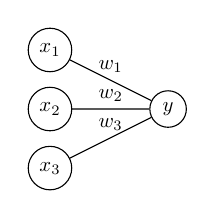
\begin{tikzpicture}[node distance=1.5cm, every node/.style={scale=0.75}, scale=0.75]

% Input layer
\foreach \i in {1,2,...,3}
	\node[circle, draw=black, minimum size=0.5cm] (x\i) at (0,4-\i) {$x_\i$};
	
% Output layer
\node[circle, draw=black, minimum size=0.5cm] (y) at (2,2) {$y$};

% Connections
\foreach \i in {1,2,...,3}
	\draw (x\i) -- node[midway,above] {$w_\i$} (y);
\end{tikzpicture}
\captionof{figure}{Linear regression model as a neural network}\label{fig:NLM}
\end{figure}

\newpage
\section{Introduction to the Bai-Silverstein Method}
The method proposed by Bai-Silverstein has the objective to determine the Hessian eigenspectra under asymptotic conditions. To accomplish this task, we find it beneficial to compile the necessary definitions and results from random matrix theory, measure theory, and complex analysis alike. For the remainder of this document, we shall denote the upper complex half-plane by 
\begin{equation}\mathbb{C}_+:=\{z\in\mathbb{C}:\operatorname{Im}(z)>0\}.
\end{equation}

\subsection{The Stieltjes Transform}
The primary focus in our analysis lies in the so-called Stieltjes tranform. Studying this object allows us to exploit the close connection between complex analysis and measure theory, providing us with the means to make concrete statements about the Hessian eigenspectrum in the asymptotic realm.
\bigskip
\begin{definition}[Stieltjes Transform]
Let $\mu$ be a probability measure. The Stieltjes transform of $\mu$ is the map $m:\mathbb{C}_+\to\mathbb{C}$ defined as
$$m(z):=\int_{\mathbb{R}}\frac{1}{\lambda-z}\,\mu(d\lambda).$$
\end{definition}
\smallskip
\par
The Stieltjes transform is an analytic function on its domain $\mathbb{C}_+$, and maps $\mathbb{C}_+$ to itself \cite{hachem}. The probability measure $\mu$ can always be reconstructed from the Stieltjes transform by applying the following inversion formula \cite{couillet, hachem}.
\bigskip
\\
\begin{theorem}[Stieltjes Inversion]
Let $a<b$ be continuity points of the cummulative distribution function of $\mu$, and let $m$ be the Stieltjes transform of $\mu$. Then
$$\mu([a,b])=\frac{1}{\pi}\lim_{\varepsilon\to0^+}\int_a^b\operatorname{Im}(m(\lambda+i\varepsilon))\,d\lambda.$$\label{thm:inversion-formula}
\end{theorem}
\bigskip
\par
The convergence of Stieltjes transform sequences is characterized by the convergence in distribution of the corresponding probability measures \cite{couillet}.
\bigskip
\begin{theorem}[Limiting Measure]\label{thm:limiting-measure}
Let $(\mu_n)_{n=1}^\infty$ be a sequence of probability measures with corresponding Stietljes transforms $(m_n)_{n=1}^\infty$. If there exists $m:\mathbb{C}_+\to\mathbb{C}_+$ such that $m$ is the Stieltjes transform of some probability measure $\mu$, and if for all $z\in\mathbb{C}_+$, almost surely as $n\to\infty$, 
$$m_n(z)\to m(z),$$
then $\mu_n\to\mu$ in distribution as $n\to\infty$. The converse statement also holds true.
\end{theorem}
\bigskip
\par
The measure $\mu$ is called the \emph{limiting measure} of the sequence $(\mu_n)_{n=1}^\infty$. Similarly, $m$ is referred to be the \emph{limiting Stieltjes transform} obtained from the sequence $(m_n)_{n=1}^\infty$.
\bigskip
\par
The convergence $m_n(z)\to m(z)$ is crucial in our analysis with large random matrices. Therefore, it is convenient to better understand the structure of the Stieltjes transform $m_n(z)$ of the empirical spectral measure $\mu_n$, given by the underlying random matrix.
\bigskip
\\
\begin{definition}[Empirical Spectral Measure]
Let $X_n\in\mathbb{R}^{n\times n}$ be a random matrix with (random) eigenvalues $\lambda_1,\dots,\lambda_n$. The empirical spectral measure of $X_n$ is defined as
$$\mu_{X_n}(A):=\frac{1}{n}\sum_{j=1}^n\delta_{\lambda_j}(A),\quad A\in\mathcal{B}(\mathbb{R}),$$
where $\delta_x(A):=\mathbf{1}_A(x)$ denotes the Dirac measure.
\end{definition}
\bigskip
\par
Connecting to Proposition \ref{thm:MP}, it is useful to see that we may equivalently express
\begin{equation}
\mu_{X_n}(A)=\frac{1}{n}\#\{\lambda_j\in A\},\quad A\in\mathcal{B}(\mathbb{R}).
\end{equation}
\smallskip
\par
As it turns out, we can represent the Stieltjes transform of the empirical spectral measure by using the trace of the so-called \emph{resolvent} matrix; yet another object that plays a central role in this thesis.
\bigskip
\\
\begin{definition}[Resolvent]
Let $X_n\in\mathbb{R}^{n\times n}$ be a random matrix. The (random) resolvent $Q_{X_n}$ of $X_n$ is defined as
$$Q_{X_n}(z):=(X_n-zI_n)^{-1},\quad z\in D(Q_{X_n}),$$
where
$$D(Q_{X_n}):=\{z\in\mathbb{C}_+:(X_n-zI_n)^{-1}\,\text{exists almost surely}\}.$$
\end{definition}
\smallskip
\par
The term $zI_n$ shifts the spectrum of $X_n$ by the complex number $z$. Indeed, if $(v,\lambda)$ is an eigenpair of $X_n$, then
\begin{equation}
(X_n-zI_n)v=X_nv-zv=(\lambda-z)v.
\end{equation}
This fact, and by choosing $z\in\mathbb{C}\setminus\mathbb{R}$ such that $z\in D(Q_{X_n})$, ensures that $X_n-zI_n$ has no zero eigenvalues and is thus invertible. When we talk about the resolvent of a matrix, we automatically assume its invertibility.
\bigskip
\\
\begin{lemma}\label{thm:stieltjes-trace-lemma}
Let $X_n\in\mathbb{R}^{n\times n}$ be a random matrix, $Q_{X_n}$ its resolvent, and
$$m_{X_n}(z)=\int_{\mathbb{R}}\frac{1}{\lambda-z}\,\mu_{x_n}(d\lambda),\quad z\in\mathbb{C}_+$$
the Stieltjes transform of the empirical spectral measure $\mu_{X_n}$.
Then,
$$m_{X_n}(z)=\frac{1}{n}\operatorname{Tr}Q_{X_n}(z)=\frac{1}{n}\sum_{j=1}^n\frac{1}{\lambda_j-z},$$
where $\lambda_1,\dots,\lambda_n$ are the eigenvalues of $X_n$.
\end{lemma}
\bigskip
\noindent
\emph{Proof.} Let $\lambda_1,\dots,\lambda_n$ be the eigenvalues of $X_n$ so that we may write
\begin{equation}
\mu_{X_n}(\lambda)=\frac{1}{n}\sum_{j=1}^n\delta(\lambda-\lambda_j).
\end{equation}
Next, we easily observe that the eigenvalues of the resolvent $Q_{X_n}(z)$ are given by $(\lambda_j-z)^{-1}$. Indeed, for every eigenpair $(\lambda_j,v_j)$ we have that
\begin{align}
v_j=Q_{X_n}(z)Q_{X_n}(z)^{-1}v_j = Q_{X_n}(z)(X_n-zI_n)v_j = Q_{X_n}(z)(\lambda_j-z)v_j,
\end{align}
yielding
\begin{equation}
Q_{X_n}(z)v_j=\frac{1}{\lambda_j-z}v_j
\end{equation}
as desired. Finally, we may conclude
\begin{align}
m_{X_n}(z) &= \int_{\mathbb{R}}\frac{\mu_{X_n}(d\lambda)}{\lambda-z} = \frac{1}{n}\sum_{j=1}^n\int_{\mathbb{R}}\frac{\delta(\lambda-\lambda_j)}{\lambda-z}\,d\lambda = \frac{1}{n}\sum_{j=1}^n\frac{1}{\lambda_j-z} = \frac{1}{n}\operatorname{Tr}Q_{X_n}(z),
\end{align}
where we used the elementary fact that the trace of a matrix is the sum of its eigenvalues, i.e. in our case
\begin{equation}
\operatorname{Tr}Q_{X_n}(z)=\sum_{j=1}^n\frac{1}{\lambda_j-z}.
\end{equation}
\qed
\bigskip
\par
A worthwhile remark about the identity
\begin{equation}
m_{X_n}(z)=\sum_{j=1}^n\frac{1}{\lambda_j-z}
\end{equation}
is that the (random) eigenvalues $\lambda_1,\dots,\lambda_n$ of $X_n$ correspond one-to-one to the discontinuity points (i.e. poles) of the complex analytic function $m_{X_n}(z)$. Therefore, one may approach the problem of finding the empirical spectral density (i.e. in the non-asymptotic regime) by studying the poles of the empirical Stieltjes transform. We refer to Srivastava et al. \cite{srivastava} for such kind of analysis.
\bigskip
\par
In our main results, we always make the key assumption that the empirical Stieltjes transform converges as the number of samples tends to infinity.
\bigskip
\begin{assumption}[Convergence of the Empirical Stieltjes Transform]\label{ass:key-assumption}
Let $X_n\in\mathbb{R}^{n\times n}$ be a symmetric, random matrix, and $Q_{X_n}(z)\in\mathbb{R}^{n\times n}$ its resolvent. Then, there exists a probability measure $\mu_X$ such that for all $z\in\mathbb{C}_+$, almost surely as $n\to\infty$,
\begin{equation}
m_{X_n}(z)=\frac{1}{n}\operatorname{Tr}Q_{X_n}(z)\to m_X(z),\label{eq:key-assumption}
\end{equation}
where $m_X(z)$ is the Stieltjes transform of $\mu_X$.\label{ass:stieltjes-convergence}
\end{assumption}
\bigskip
\par
The following property of the Stieltjes transform, also found in \cite{hachem}, is an essential technical detail for the analysis performed in this work due to its usage in the proofs of our main results, where we need to quantify the operator norm of particular matrices.
\bigskip
\begin{definition}[Operator Norm]
Let $A\in\mathbb{R}^{n\times n}$ be an arbitrary matrix. Then we define its operator norm as
$$\left\|A\right\|:=\sup_{v\in\mathbb{R}^n:\left\|v\right\|=1}\left\|Av\right\|.$$
\end{definition}
\bigskip
\begin{lemma}
Let $m:\mathbb{C}_+\to\mathbb{C}_+$ be the Stieltjes transform of some probability measure $\mu$. Then
$$|m(z)|\,\leq\frac{1}{d(z,\operatorname{supp}(\mu))}$$
for all $z\in\mathbb{C}_+$, where
$$d(z,\operatorname{supp}(\mu)):=\inf\limits_{x\in\operatorname{supp}(\mu)}|z-x|$$
denotes the complex Euclidean distance.\label{thm:stieltjes-bounded}
\end{lemma}
\bigskip
\noindent
\emph{Proof.} Let $z\in\mathbb{C}_+$ be arbitrary. By definition of the Stieltjes transform,
\begin{align}
|m(z)|\,&=\left|\int_{\mathbb{R}}\frac{1}{\lambda-z}\,\mu(d\lambda)\right| \notag
\\ &\leq\left|\int_{\mathbb{R}}\frac{1}{d(z,\operatorname{supp}(\mu))}\,\mu(d\lambda)\right|\,=\frac{1}{d(z,\operatorname{supp}(\mu))}\,\underbrace{\int_{\mathbb{R}}\mu(d\lambda)}_{=1},
\end{align}
using that $\mu$ is normalized, and that $\operatorname{supp}(\mu)\subseteq\mathbb{R}$.
\qed
\bigskip
\\
\emph{An important remark:} In the same way as explained by Couillet et al. in Remark 2.1 of \cite{couillet}, we may bound the operatorn norm $\|Q_{X_n}(z)\|\leq d(z,\operatorname{supp}(\mu_n))^{-1}$ as $n\to\infty$, after bounding the empirical Stieltjes transform $m_{X_n}(z)$ as in Lemma \ref{thm:stieltjes-bounded}. We use this particularly for bounding the spectral norm of the resolvent
\begin{equation}
\|Q_{x_n}(z)\|\leq \frac{1}{d(z,\operatorname{supp}(\mu_n))}\leq\frac{1}{\operatorname{Im}(z)}=\mathcal{O}(1) \label{eq:important-remark}
\end{equation}
as $n\to\infty$, using $\operatorname{supp}(\mu_n)\subseteq\mathbb{R}$ for all $n\geq1$.

\subsection{The Deterministic Equivalent} \label{sec:deterministic-equivalent}
The concept of the so-called \emph{deterministic equivalent} $\overline{Q_{X_n}}(z)$ of the resolvent $Q_{X_n}(z)$ is the key object for finding a self-consistent equation for the limiting Stieltjes transform $m_X(z)$. The idea behind this concept is to fix an arbitrary $z\in\mathbb{C}_+$, and then find a deterministic matrix $\overline{Q_{X_n}}(z)\in\mathbb{R}^{n\times n}$ such that, almost surely as $n\to\infty$,
\begin{equation}
\frac{1}{n}\operatorname{Tr}\left(Q_{X_n}(z)- \overline{Q_{X_n}}(z)\right)\to0\quad\text{and}\quad\|\overline{Q_{X_n}}(z)\|\,\leq\mathcal{O}(1).\label{eq:deterministic-equivalent}
\end{equation}
\bigskip
\par
The latter statement in (\ref{eq:deterministic-equivalent}) is needed for a technical argument. The former is where we use the key assumption (\ref{eq:key-assumption}): Let $z\in\mathbb{C}_+$ be arbitrary. Then, almost surely,
\begin{align}
m_X(z)-\lim_{n\to\infty}\frac{1}{n}\operatorname{Tr}\overline{Q_{X_n}}(z) &\stackrel{(\ref{eq:key-assumption})}{=} \lim_{n\to\infty}m_{X_n}(z)-\frac{1}{n}\operatorname{Tr}\overline{Q_{X_n}}(z) \notag
\\ & \stackrel{\ref{thm:stieltjes-trace-lemma}}{=} \lim_{n\to\infty}\frac{1}{n}\operatorname{Tr}\left(Q_{X_n}(z)-\overline{Q_{X_n}}(z)\right)\stackrel{(\ref{eq:deterministic-equivalent})}{=}0.
\end{align}
This means that we can express the limiting Stieltjes transform
\begin{equation}
m_X(z)=\lim_{n\to\infty}\frac{1}{n}\operatorname{Tr}\overline{Q_{X_n}}(z)\label{eq:m=TrQ}
\end{equation}
in terms of the deterministic equivalent $\overline{Q_{X_n}}(z)$, which is what we need to derive the self-consistent equation for $m_X(z)$. By employing techniques from random matrix theory, and concentration inequalities, we derive an equation which allows us to explicitly determine $\overline{Q_{X_n}}(z)$ such that the first statement in (\ref{eq:deterministic-equivalent}) holds true.

\subsection{Lemmata for the Bai-Silverstein Analysis}
We will make use of the following four lemmata which can be found in \cite{couillet} and are essentially the main ideas behind the Bai-Silverstein analysis.
\bigskip
\par
First, let us clarify the following notation: For a matrix $A\in\mathbb{R}^{d\times d}$ we denote $\|A\|:=\sup_{\|x\|=1}\|Ax\|$ to be the spectral norm. Moreover, for two random variables $x_n,y_n\in\mathbb{R}$ we say that $x_n\simeq y_n$ almost surely as $n\to\infty$ if $P\left(\lim_{n\to\infty}|x_n-y_n|\,=0\right)=1$. In particular, if $x_n\simeq y_n$, then also have that $f(x_n)\simeq f(y_n)$ for any continuous $f:\mathbb{R}\to\mathbb{R}$.
\par
Moreover, we shall frequently use the following "partial asymptoticity" argument: If $x_n\to x$ and $y_n\to y$ almost surely as $n\to\infty$, then $f(x_n,y_n)\simeq f(x,y_n)\simeq f(x_n,y)\to f(x,y)$, almost surely as $n\to\infty$, for any continuous $f:\mathbb{R}^2\to\mathbb{R}$.
\bigskip
\\
\begin{lemma}[Resolvent Identity]\label{thm:resolvent}
Let $A,B\in\mathbb{R}^{d\times d}$ be two invertible matrices. Then
$$A^{-1}-B^{-1}=A^{-1}(B-A)B^{-1}.$$
\end{lemma}
\bigskip
\noindent
\begin{lemma}[Sherman-Morrison Lemma]\label{thm:SM}
Let $A\in\mathbb{R}^{d\times d}$ be an invertible matrix, and $u,v\in\mathbb{R}^d$. Then $A+uv^\top$ is invertible if and only if $1+v^\top A^{-1}u\neq0$, and
$$(A+uv^\top)^{-1}=A^{-1}-\frac{A^{-1}uv^\top A^{-1}}{1+v^\top A^{-1}u}.$$
Moreover,
$$(A+uv^\top)^{-1}u=\frac{A^{-1}u}{1+v^\top A^{-1}u}.$$
\end{lemma}
\bigskip
\par
The second statement in the following lemma explains why we are interested in the bounds $\|Q_{X_n}(z)\|\,\leq\mathcal{O}(1)$ and $\|\overline{Q_{X_n}}(z)\|\,\leq\mathcal{O}(1)$ as $n\to\infty$, previously discussed in (\ref{eq:important-remark}) and (\ref{eq:deterministic-equivalent}), respectively.
\bigskip
\noindent
\begin{lemma}[Bai-Silverstein Rank-1 Perturbation]\label{thm:rank-1-perturbation}
Let $A,M\in\mathbb{R}^{d\times d}$ be symmetric matrices, $u\in\mathbb{R}^d$, $\tau\in\mathbb{R}$ and $z\in\mathbb{C}_+$ all be arbitrary. Then
$$|\operatorname{Tr}A(M+\tau uu^\top-zI_d)^{-1}-\operatorname{Tr}A(M-zI_d)^{-1}|\leq\frac{\|A\|}{\operatorname{Im}(z)}.$$
In particular, if $\|A\|\leq\mathcal{O}(1)$ as $d\to\infty$, then
$$\frac{1}{d}\operatorname{Tr}\left(AQ_{M+\tau uu^\top}(z)\right)\simeq\frac{1}{d}\operatorname{Tr}\left(AQ_M(z)\right)$$
as $d\to\infty$.
\end{lemma}
\bigskip
\par
Lemma \ref{thm:trace-lemma} below is by far the most important one in our analysis. We use it to concentrate quadratic forms involving the resolvent, so that we may rewrite it in terms of the trace of the resolvent in the regime $d\to\infty$. Recalling (\ref{eq:m=TrQ}), we see that this is indeed a convenient method for finding a self-consistent equation for the limiting Stieltjes transform $m(z)$.
\bigskip
\bigskip
\\
\textbf{Assumptions on the Data.} Throughout this thesis, we always assume that the entries of the random data matrix $X=[x_1,\dots,x_n]\in\mathbb{R}^{d\times n}$ are i.i.d. with zero mean, unit variance, and finite eighth order moments. Despite the fact that these conditions are required in Lemma \ref{thm:trace-lemma} below, we also need it for other technical arguments when considering the two-layer network in Section \ref{sec:two-layer} below.
\bigskip
\begin{assumption}[Data Assumptions]\label{ass:data}
The entries $X_{ij}$ of the random data matrix $X=[x_1,\dots,x_n]\in\mathbb{R}^{d\times n}$ are i.i.d. with zero mean, unit variance, and finite eighth order moments, i.e.
$$\mathbb{E}[X_{ij}]=0,\quad \mathbb{E}[X_{ij}^2]=1,\quad \mathbb{E}[|X_{ij}|^8]<\infty.$$
In particular, $\mathbb{E}[x_\ell x_\ell^\top]=I_d$ for all $\ell=1,\dots,n$.
\end{assumption}
\bigskip
\noindent
\begin{lemma}[Bai-Silverstein Trace Concentration, Lemma B.26 in \cite{bai}]\label{thm:trace-lemma}
Let $x\in\mathbb{R}^d$ be a random vector with independent entries $x_i$ of zero mean and unit variance with $\mathbb{E}[|x_i|^K]\leq\nu_K$ for some $K\geq 4$ and a corresponding constant $\nu_K>0$. Then for any matrix $A\in\mathbb{R}^{d\times d}$ with $\operatorname{Tr}(AA^\top)\leq\mathcal{O}(d)$ as $d\to\infty$, and $k\leq K$ we have
$$\mathbb{E}\left[\left|x^\top A x-\operatorname{Tr}A\right|^k\right]\leq C_k\left[\left(\nu_4\operatorname{Tr}(AA^\top)\right)^{k/2}+\nu_{2k}\operatorname{Tr}\left(AA^\top\right)^{k/2}\right]$$
for some $C_k>0$ independent of $d$. In particular, if the entries of $x$ have bounded eighth-order moment, then
$$\mathbb{E}\left[\left(\frac{1}{d}x^\top Ax-\frac{1}{d}\operatorname{Tr}A\right)^4\right]\leq\mathcal{O}(d^{-2}),$$
which consequently yields, almost surely as $d\to\infty$,
$$\frac{1}{d}x^\top Ax\simeq\frac{1}{d}\operatorname{Tr}A.$$
\end{lemma}
\bigskip
\par
The assumption that $\operatorname{Tr}(AA^\top)\leq\mathcal{O}(d)$ is very important. Applying the first statement of the lemma with $k=4$ yields that $\mathbb{E}\left[\left|x^\top A x-\operatorname{Tr}A\right|^k\right]\leq\mathcal{O}(d^2)$. Therefore, multiplying the difference between the quadratic form and the trace with the factor $1/d$ indeed gives the desired bound $\mathcal{O}(d^{-2})$ in the second statement. Next, denoting $u_d:=\frac{1}{d}x^\top A x-\frac{1}{d}\operatorname{Tr}A$, Markov's inequality implies that for all $\varepsilon>0$,
\begin{equation}
P(|u_d|>\varepsilon)=P(|u_d|^4>\varepsilon^2)\leq\frac{\mathbb{E}[|u_d|^4]}{\varepsilon^4}\leq\mathcal{O}(d^{-2}).
\end{equation}
Therefore, for all $\varepsilon>0$,
\begin{equation}
\sum_{d=1}^\infty P(|u_d|>\varepsilon)<\infty,
\end{equation}
which means that we can use the Borel-Cantelli Lemma, and conclude with $u_d\stackrel{a.s.}{\to}0$ as $d\to\infty$.
\bigskip
\par
Concentration inequalities for quadratic forms in the sense that
\begin{equation}
P_x(x^\top A x-\mathbb{E}[x^\top A x]\geq t)\leq c(t),
\end{equation}
for some quantitative $c:\mathbb{R}\to\mathbb{R}$, allowing us to conclude with almost sure convergence, are beneficial tools \cite{couillet, rudelson, louart}. In fact, our concentration argument in Lemma \ref{thm:trace-lemma} is of a very similar form. Indeed, if the matrix $A$ is independent of the random vector $x$, then
\begin{align}
\mathbb{E}[x^\top A x] &= \mathbb{E}\left[\sum_{i,j=1}^n x_iA_{ij}x_j\right]=\sum_{i,j=1}^nA_{ij}\underbrace{\mathbb{E}[x_ix_j]}_{=\delta_{ij}}=\sum_{i=1}^nA_{ii}=\operatorname{Tr}(A).
\end{align}



\newpage
\section{Nonlinear Regression Model} \label{sec:NLRM}
Having explored the spectral analysis in the context of linear regression, and gained insights from the foundational theory of neural networks, we can now try to extend our analysis to a slightly more generalized model; a single-layer neural network with a nonlinear activation function $\phi$.
\bigskip
\par
The loss function of the model is given by
\begin{equation}
\mathcal{L}(w):=\frac{1}{2n}\sum_{i=1}^n(\phi(w^\top x_i)-y_i)^2=\frac{1}{2n}\|\phi(X^\top w)-y\|^2.\label{eq:loss-NLRM}
\end{equation}
Here, we use the random data matrix $X:=[x_1,\dots,x_n]\in\mathbb{R}^{d\times n}$ and the target vector $y:=[y_1,\dots,y_n]^\top\in\mathbb{R}^n$ just as before. The weight vector $w\in\mathbb{R}^d$ is yet again the only trainable parameter in our model, that is $\theta\equiv w$. We assume that the activation function $\phi:\mathbb{R}\to\mathbb{R}$ is almost surely twice differentiable.

\subsection{Matrix Structure of the Hessian}
Prior to the spectral analysis of the Hessian, we need to explicitly understand its structure. In this section, we thus derive that the Hessian of the model (\ref{eq:loss-NLRM}) is a weighted sum of the rank-1 matrices $x_\ell x_\ell^\top$.
\bigskip
\begin{proposition}\label{thm:NLRM-Hessian}
The Hessian matrix of the loss (\ref{eq:loss-NLRM}) is of the form
$$\mathcal{H}(w)=\mathcal{H}_1(w)+\mathcal{H}_2(w),$$
where
$$(\mathcal{H}_1)_{ij}(w)=\frac{1}{n}\sum_{k=1}^n\phi'(w^\top x_k)^2\cdot(x_k)_i(x_k)_j$$
and
$$(\mathcal{H}_2)_{ij}(w)=\frac{1}{n}\sum_{k=1}^n\phi''(w^\top x_k)(\phi(w^\top x_k)-y_k)\cdot(x_k)_i(x_k)_j.$$
\end{proposition}
\smallskip
\noindent
\emph{Proof.} First, we compute the gradient using the chain rule
\begin{align}
\frac{\partial\mathcal{L}(w)}{\partial w_i} &= \frac{1}{2n}\sum_{k=1}^n\frac{\partial}{\partial w_i}(\phi(w^\top x_k)-y_k)^2 = \frac{1}{n}\sum_{k=1}^n(\phi(w^\top x_k)-y_k)\cdot\frac{\partial}{\partial w_i}\phi(w^\top x_k) \notag
\\ &= \frac{1}{n}\sum_{k=1}^n(\phi(w^\top x_k)-y_k)\cdot\phi'(w^\top x_k)(x_k)_i.
\end{align}
Therefore, by the product rule
\begin{align}
\frac{\partial^2\mathcal{L}(w)}{\partial w_i\partial w_j} &= \frac{1}{n}\sum_{k=1}^n\frac{\partial}{\partial w_j}\left((\phi(w^\top x_k)-y_k)\cdot\phi'(w^\top x_k)(x_k)_i\right) \notag
\\ &= \frac{1}{n}\sum_{k=1}^n\left\{\frac{\partial}{\partial w_j}\phi(w^\top x_k)\cdot\phi'(w^\top x_k)(x_k)_i+(\phi(w^\top x_k)-y_k)\cdot\frac{\partial}{\partial w_j}\phi'(w^\top x_k)(x_k)_i\right\} \notag
\\ &= \frac{1}{n}\sum_{k=1}^n\left\{\phi'(w^\top x_k)^2(x_k)_i(x_k)_j+(\phi(w^\top x_k)-y_k)\phi''(w^\top x_k)(x_k)_i(x_k)_j \right\} \notag
\\ &= \frac{1}{n}\sum_{k=1}^n\left\{\phi'(w^\top x_k)^2+\phi''(w^\top x_k)(\phi(w^\top x_k)-y_k)\right\}\cdot(x_k)_i(x_k)_j,
\end{align}
from which the statement easily follows.
\qed
\bigskip
\par
From the representations found in Proposition \ref{thm:NLRM-Hessian}, and by the fact that
\begin{equation}
xx^\top = \begin{bmatrix} x_1 \\ x_2 \\ \vdots \\ x_d \\ \end{bmatrix} \begin{bmatrix} x_1 & x_2 & \cdots & x_d \\ \end{bmatrix} = \begin{bmatrix} x_1^2 & x_1x_2 & \cdots & x_1x_d \\ x_2x_1 & x_2^2 & \cdots & x_2x_d \\ \vdots & \vdots & \ddots & \vdots \\ x_dx_1 & x_dx_2 & \cdots & x_d^2 \\ \end{bmatrix}
\end{equation}
for any $x\in\mathbb{R}^d$, it is not hard to see that we can directly write
\begin{align}
\mathcal{H}_1(w)=\frac{1}{n}X \begin{bmatrix} \phi'(w^\top x_1)^2 & & 0 \\ & \ddots & \\ 0 & & \phi'(w^\top x_n)^2\end{bmatrix} X^\top=\frac{1}{n}\sum_{k=1}^n\phi'(w^\top x_k)^2x_kx_k^\top,
\end{align}
and analogously
\begin{align}
\mathcal{H}_2(w) &= \frac{1}{n}\sum_{k=1}^n\phi''(w^\top x_k)(\phi(w^\top x_k)-y_k)x_kx_k^\top.
\end{align}
\bigskip
\par
When choosing the identity $\phi(z)=z$, we obtain the linear regression model since $\phi'(z)=1$ and $\phi''(z)=0$ resulting in
\begin{equation}
\mathcal{H}(w)=\mathcal{H}_1(w)+\mathcal{H}_2(w)=\frac{1}{n}X I_nX^\top+0=\frac{1}{n}XX^\top,
\end{equation}
as found in Proposition \ref{thm:covariance}.
\bigskip
\par
The second term $\mathcal{H}_2(w)$ contains all second derivatives of $\phi$, and the residuals 
\\
$\phi(w^\top x_k)-y_k$. Furthermore, it is evident that both $\mathcal{H}_1(w)$ and $\mathcal{H}_2(w)$ are symmetric matrices.
\bigskip
\\
\begin{lemma}
The matrix $\mathcal{H}_1(w)$ is positive semi-definite.
\end{lemma}
\bigskip
\noindent
\emph{Proof.} Indeed, we have for all $v\in\mathbb{R}^d$ that
\begin{equation}
v^\top\mathcal{H}_1(w)v=\frac{1}{n}\sum_{k=1}^n\phi'(w^\top x_k)^2v^\top x_kx_k^\top v=\frac{1}{n}\sum_{k=1}^n\phi'(w^\top x_k)^2(v^\top x_k)^2\geq0.
\end{equation}
\qed
\bigskip
\par
In general, $\mathcal{H}_2$ is not positive semi-definite: For all $v\in\mathbb{R}^d$ we see
\begin{align}
v^\top\mathcal{H}_2(w)v&=\frac{1}{n}\sum_{k=1}^n\phi''(w^\top x_k)(\phi(w^\top x_k)-y_k)v^\top x_kx_k^\top v \notag
\\ &= \frac{1}{n}\sum_{k=1}^n\phi''(w^\top x_k)(\phi(w^\top x_k)-y_k)(v^\top x_k)^2,
\end{align}
illustrating how the sign of the eigenvalues of $\mathcal{H}_2(w)$ depends on the coefficients \\$\phi''(w^Tx_k)(\phi(w^\top x_k)-y_k)$ in the weighted sum above. For example, in the case where $\phi(z)=z^2$ is quadratic, then the sign of the eigenvalues only depends on the residuals $(w^\top x_k)^2-y_k$.
\bigskip
\par
The goal of our subsequent analysis is to provide an explicit solution for the eigenvalue distribution of $\mathcal{H}(w)$ in the asymptotic regime $n,d\to\infty$.
\bigskip
\bigskip
\\
\textbf{The Marchenko-Pastur Law.} We are now fully equipped to formulate the Marchenko-Pastur law. Its subsequent discussion justifies Proposition \ref{thm:MP}. The Marchenko-Pastur law is a special case of our first main result, Theorem \ref{thm:mainresult-1} further below.
\bigskip
\\
\begin{theorem}[Marchenko-Pastur Stieltjes Transform]\label{thm:MP-stieltjes}
Let $X_d\in\mathbb{R}^{d\times n}$ be a sequence of random matrices satisfying Assumption \ref{ass:data}, and $Q_d(z)$ be the resolvent of $\frac{1}{n}X_dX_d^\top$. By Assumption \ref{ass:key-assumption} we require that there exists a Stieltjes transform $m$ (of some probability measure $\mu$) such that 
$$m_d(z):=\frac{1}{d}\operatorname{Tr}Q_d(z)\stackrel{a.s.}{\to}m(z)$$
for all $z\in\mathbb{C}_+$ as $n,d\to\infty$, where $n/d\to\alpha\in(1,\infty)$. Then the limiting Stieltjes transform $m(z)$ satisfies the fixed point equation
$$\frac{z}{\alpha}m(z)^2-\left(1-\frac{1}{\alpha}-z\right)m(z)+1=0.$$
\end{theorem}
\smallskip
\noindent
\emph{Proof.} This directly follows from Theorem \ref{thm:mainresult-1} below with $\phi=\operatorname{id}$.
\qed
\bigskip
\par
The fixed point equation is simply a quadratic equation in $m(z)$ which can be solved uniquely due to the fact that $\operatorname{Im}(m(z))>0$ if $\operatorname{Im}(z)>0$. The solution is given by
\begin{equation}
m(z)=\frac{\alpha}{2z}(1-\alpha^{-1}-z)-\frac{\alpha}{2z}\sqrt{((1-\sqrt{\alpha^{-1}})^2-z)((1+\sqrt{\alpha^{-1}})^2-z)}.
\end{equation}
The points of discontinuity are given by $0$ and $(1\pm\sqrt{\alpha^{-1}})^2$. All eigenvalues must be real, thus we may conclude that
\begin{equation}
\operatorname{supp}(\mu)=\left[(1-\sqrt{\alpha^{-1}})^2,(1+\sqrt{\alpha^{-1}})^2\right].
\end{equation}
In particular, the edges of the support of $\mu$ are given by
\begin{equation}
\lambda_\pm(\alpha)=(1\pm\sqrt{\alpha^{-1}})^2.
\end{equation}
\bigskip

\subsection{Spectral Analysis of the Hessian}\label{sec:mainresult1}
Let us return to Proposition \ref{thm:NLRM-Hessian}, where we found the Hessian of the nonlinear regression model,
\begin{equation}
\mathcal{H}(w)=\frac{1}{n}\sum_{\ell=1}^n\tau_\ell(w)x_\ell x_\ell^\top,
\end{equation}
where, for fixed $w\in\mathbb{R^d}$, we introduce the random variables $\tau_\ell(w)\in\mathbb{R}$ given by
\begin{equation}
\tau_\ell(w):=\phi'(w^\top x_\ell)^2+\phi''(w^\top x_\ell)(\phi(w^\top x_\ell)-y_\ell).\label{eq:def-tau}
\end{equation}
\par
The Hessian is a weighted sum of the rank-one matrices $x_\ell x_\ell^\top$. This means that the Hessian $\mathcal{H}$ is of the form we need for the previously presented Bai-Silverstein lemmata. We remind the reader that we always assume the key assumption, Assumption \ref{ass:key-assumption}, ensuring the convergence of the empirical Stieltjes transform to the limiting Stieltjes transform, denoted by $m(z)$.
\bigskip
\begin{theorem}[Main Result I]\label{thm:mainresult-1} Let $X=[x_1,\dots,x_n]\in\mathbb{R}^{d\times n}$ satisfy Assumption \ref{ass:data}, and $w\in\mathbb{R}^d$ be arbitrary. Let $Q_d(z)$ be the resolvent of $\mathcal{H}(w)$, and assume that there exists a function $F:\mathbb{C}_+\to\mathbb{C}_+$ such that
$$F_n(z):=\frac{1}{n}\sum_{\ell=1}^n \frac{\tau_\ell(w)}{1+\frac{\tau_\ell(w)}{\alpha}z}\stackrel{a.s.}{\to}F(z)$$
point-wise as $n,d\to\infty$, where $n/d\to\alpha\in(1,\infty)$. Then the limiting Stieltjes transform $m(z)$ satisfies the fixed point equation
$$m(z)=\frac{1}{F(m(z))-z}$$
for all $z\in\mathbb{C}_+$.
\end{theorem}
\bigskip
\noindent
\emph{Proof.} Let $z\in\mathbb{C}_+$ be arbitrary. By Assumption \ref{ass:key-assumption}, we know that the limiting Stieltjes transform $m(z)$ is determined by
$$m_d(z):=\frac{1}{d}\operatorname{Tr}Q_d(z)\stackrel{a.s.}{\to}m(z),$$
as $d\to\infty$. Therefore, it is a well-defined problem trying to find a solution $\overline{Q_d}(z)\in\mathbb{R}^{d\times d}$ of
\begin{equation}
\frac{1}{d}\operatorname{Tr}Q_d(z)\simeq\frac{1}{d}\operatorname{Tr}\overline{Q_d}(z)\quad\text{and}\quad\|\overline{Q_d}(z)\|\,\leq\mathcal{O}(1),\label{eq:deterministic-equiv}
\end{equation}
almost surely as $d\to\infty$. To solve the problem above, we will proceed as elaborated in Section \ref{sec:deterministic-equivalent}: The idea is that the first property in (\ref{eq:deterministic-equiv}) allows us to establish an explicit expression for $\overline{Q_d}(z)$, relating it to $m(z)$. The second property in (\ref{eq:deterministic-equiv}) is solely needed for technical details. First, we start by exploiting the resolvent identity, Lemma \ref{thm:resolvent}, in order to establish the identity
\begin{align}
Q_d(z)-\overline{Q_d}(z) &= Q_d(z)\left(\overline{Q_d}(z)^{-1}-Q_d(z)^{-1}\right)\overline{Q_d}(z) \notag
\\ &= Q_d(z)\left(\overline{Q_d}(z)^{-1}+zI_d-\frac{1}{n}\sum_{\ell=1}^n \tau_\ell(w) x_\ell x_\ell^\top\right)\overline{Q_d}(z).
\end{align}
Therefore, almost surely as $d\to\infty$, using (\ref{eq:deterministic-equiv}) and the cyclic property of the trace operator,
\begin{align}
0&\simeq\frac{1}{d}\operatorname{Tr}\left(Q_d(z)-\overline{Q_d}(z)\right) =\frac{1}{d}\operatorname{Tr}\left(Q_{d}(z)\left(\overline{Q_{d}}(z)^{-1}+zI_{d}-\frac{1}{n}\sum_{\ell=1}^n\tau_\ell(w) x_\ell x_\ell^\top\right)\overline{Q_{d}}(z)\right) \notag
\\&= \frac{1}{d}\operatorname{Tr}\left(\left(\overline{Q_{d}}(z)^{-1}+zI_{d}-\frac{1}{n}\sum_{\ell=1}^n\tau_\ell(w) x_\ell x_\ell^\top\right)\overline{Q_{d}}(z)Q_{d}(z)\right) \notag
\\&= \frac{1}{d}\operatorname{Tr}\left((zI_{d}+\overline{Q_{d}}(z)^{-1})\overline{Q_{d}}(z)Q_{d}(z)\right)-\frac{1}{dn}\sum_{\ell=1}^n\tau_\ell(w)\operatorname{Tr}\left(x_\ell x_\ell^\top\overline{Q_d}(z)Q_d(z)\right).
\end{align}
\par
At this point, the key observation is that a quadratic form emerges from the elementary fact that
\begin{equation}
\operatorname{Tr}(x_\ell x_\ell^\top\overline{Q_d}(z)Q_d(z)) = x_\ell^\top\overline{Q_d}(z)Q_d(z)x_\ell,
\end{equation}
opening the door for the crucial concentration arguments further below.
\par
Consequently, we find
\begin{equation}
\frac{1}{d}\operatorname{Tr}\left((zI_d+\overline{Q_d}(z)^{-1})\overline{Q_d}(z)Q_d(z)\right)\simeq \frac{1}{dn}\sum_{\ell=1}^n\tau_\ell(w) x_\ell^\top\overline{Q_d}(z)Q_d(z)x_\ell.\label{eq:trace-sim}
\end{equation}
\par
Unfortunately, the random matrix $\overline{Q_d}(z)Q_d(z)$ generally depends on $x_\ell$ for $\ell=1,\dots,n$, which prevents us from directly applying Lemma \ref{thm:trace-lemma} with $A=\overline{Q_d}(z)Q_d(z)$. Instead, we need to make an additional technical argument: Separately, for each $\ell=1,\dots,n$, we introduce the ''leave-one-out''-modification
\begin{equation}
Q_d^{-\ell}(z):=\left(-zI_d + \frac{1}{n}\sum_{\substack{k=1 \\ k\neq\ell}}^n\tau_k(w) x_kx_k^\top\right)^{-1}
\end{equation}
of the resolvent $Q_d(z)$, with the purpose of guaranteeing the independence between $Q_d^{-\ell}(z)$ and $x_\ell$. 
\par
Another key observation is that the inverse of each $Q^{-\ell}_d(z)$ only differs by the rank-1 perturbation $\frac{1}{n}\tau_\ell(w) x_\ell x_\ell^\top$ from the inverse of the original resolvent $Q_d(z)$. More precisely,
\begin{equation}
Q_d(z)^{-1} = -zI_d+\frac{1}{n}\sum_{\substack{k=1 \\ k\neq\ell}}^n\tau_k(w) x_kx_k^\top+\frac{1}{n}\tau_\ell(w) x_\ell x_\ell^\top = Q_d^{-\ell}(z)^{-1}+\frac{1}{n}\tau_\ell(w) x_\ell x_\ell^\top.
\end{equation}
This trick motivates the use of Lemma \ref{thm:rank-1-perturbation} later on, which is in fact only used for making this technical argument, paving the way for the concentration arguments discussed earlier.
\bigskip
\par
If we want to derive a self consistent equation in $m(z)$, the empirical Stieltjes transform $\frac{1}{d}\operatorname{Tr}Q_d(z)\simeq m(z)$ somehow has to emerge in our computations above. This can be done with the help of Sherman-Morrison lemma,
\bigskip
\par
We concretely apply Lemma \ref{thm:SM} to $u=x_\ell$, $v=\frac{\tau_\ell(w)}{n}x_\ell$ and $A=-zI_d+\frac{1}{n}\sum\limits_{k\neq\ell}\tau_k(w) x_kx_k^\top$ (i.e. $A^{-1}=Q_d^{-\ell}(z)$), resulting into the key identity
\begin{equation}
Q_d(z)x_\ell = \frac{Q_d^{-\ell}(z)x_\ell}{1+\frac{\tau_\ell(w)}{n}x_\ell^\top Q_d^{-\ell}(z)x_\ell},
\end{equation}
which--in combination with the concentration arguments--will indeed lead us to the desired fixed point equation for $m(z)$.
\bigskip
\par
Let us return to (\ref{eq:trace-sim}), and establish the equation--mentioned in the beginning--that allows us to solve for $\overline{Q_d}(z)$.
 \begin{align}
\frac{1}{dn}\sum_{\ell=1}^n\tau_\ell(w)  x_\ell^\top\overline{Q_d}(z)\cdot Q_d(z)x_\ell &= \frac{1}{dn}\sum_{\ell=1}^n\tau_\ell(w) x_\ell^\top\overline{Q_d}(z)\cdot \frac{Q_d^{-\ell}(z)x_\ell}{1+\frac{\tau_\ell(w)}{n}x_\ell^\top Q_d^{-\ell}(z)x_\ell} \notag
\\ &= \frac{1}{n}\sum_{\ell=1}^n\frac{\tau_\ell(w)}{1+\frac{\tau_\ell(w)}{n}x_\ell^\top Q_d^{-\ell}(z)x_\ell}\cdot\frac{1}{d}x_\ell^\top\overline{Q_d}(z)Q_d^{-\ell}(z)x_\ell \notag
\\ &\simeq \frac{1}{n}\sum_{\ell=1}^n\frac{\tau_\ell(w)}{1+\frac{\tau_\ell(w)}{\alpha}m(z)}\cdot\frac{1}{d}x_\ell^\top\overline{Q_d}(z)Q_d^{-\ell}(z)x_\ell \label{eq:BS-argument1}
\\ &\simeq \frac{1}{n}\sum_{\ell=1}^n\frac{\tau_\ell(w)}{1+\frac{\tau_\ell(w)}{\alpha}m(z)}\cdot\frac{1}{d}\operatorname{Tr}(\overline{Q_d}(z)Q_d(z)) \label{eq:BS-argument2}
\\ &= \frac{1}{d}\operatorname{Tr}\left(\left(\frac{1}{n}\sum_{\ell=1}^n\frac{\tau_\ell(w)}{1+\frac{\tau_\ell(w)}{\alpha}m(z)}\right)\overline{Q_d}(z)Q_d(z)\right). \notag
\end{align}
The equivalence in (\ref{eq:BS-argument1}) above is derived with Lemmata \ref{thm:rank-1-perturbation} and \ref{thm:trace-lemma} as follows:
\begin{equation}
\frac{1}{n}x_\ell^\top Q_d^{-\ell}(z)x_\ell \stackrel{\ref{thm:trace-lemma}}{\simeq} \frac{1}{n}\operatorname{Tr}Q_d^{-\ell}(z)=\frac{d}{n}\cdot\frac{1}{d}\operatorname{Tr}Q_d^{-\ell}(z)\stackrel{\ref{thm:rank-1-perturbation}}{\simeq}\frac{1}{\alpha}\cdot\frac{1}{d}\operatorname{Tr}Q_d(z) \simeq\frac{1}{\alpha}m(z)
\end{equation}
for all $\ell=1,\dots,n$, almost surely as $n,d\to\infty$. Note that we also used $n/d\to\alpha$ and $\operatorname{Tr}Q_d(z)/d\to m(z)$ almost surely as $n,d\to\infty$. In a similar manner, we obtain the equivalence in (\ref{eq:BS-argument2}) from
\begin{equation}
\frac{1}{d}x_\ell^\top\overline{Q_d}(z)Q_d^{-\ell}(z)x_\ell \stackrel{\ref{thm:trace-lemma}}{\simeq} \frac{1}{d}\operatorname{Tr}\left(\overline{Q_d}(z)Q_d^{-\ell}(z)\right) \stackrel{\ref{thm:rank-1-perturbation}}{\simeq} \frac{1}{d}\operatorname{Tr}\left(\overline{Q_d}(z)Q_d(z)\right)
\end{equation}
for all $\ell=1,\dots,n$, almost surely as $n,d\to\infty$.
\bigskip
\par
Note that the application of Lemma \ref{thm:rank-1-perturbation} is justified since $A\in\{I_d,\overline{Q_d}(z)\}$ satisfies $\|A\|\leq\mathcal{O}(1)$. On the other hand, we still need to prove why we can apply Lemma \ref{thm:trace-lemma} with $A\in\{Q_d^{-\ell},\overline{Q_d}(z)Q_d^{-\ell}(z)\}$ which requires that $\operatorname{Tr}(AA^\top)\leq\mathcal{O}(d)$. We will return to this technical argument at the end of the proof.
\bigskip
\par
Finally, we may combine (\ref{eq:trace-sim}) and (\ref{eq:BS-argument1}), leaves us with
\begin{align}
\frac{1}{d}\operatorname{Tr}\left((zI_d+\overline{Q_d}(z)^{-1})\overline{Q_d}(z)Q_d(z)\right) &\simeq \frac{1}{dn}\sum_{\ell=1}^n\tau_\ell(w) x_\ell^\top\overline{Q_d}(z)Q_d(z)x_\ell
\\ &\simeq \frac{1}{d}\operatorname{Tr}\left(\left(\frac{1}{n}\sum_{\ell=1}^n\frac{\tau_\ell(w)}{1+\frac{\tau_\ell(w)}{\alpha}m(z)}\right)\overline{Q_d}(z)Q_d(z)\right) \notag
\end{align}
and we may thus establish
\begin{equation}
zI_d+\overline{Q_d}(z)^{-1}\stackrel{!}{=}\left(\frac{1}{n}\sum_{\ell=1}^n\frac{\tau_\ell(w)}{1+\frac{\tau_\ell(w)}{\alpha}m(z)}\right)I_d=F_n(m(z))I_d.
\end{equation}
The solution $\overline{Q_d}(z)$ to this equation, such that $\frac{1}{d}\operatorname{Tr}Q_d(z)\simeq\frac{1}{d}\operatorname{Tr}\overline{Q_d}(z)$ to holds true, is simply given by the scaled identity matrix
\begin{equation}
\overline{Q_d}(z):=\frac{1}{F_n(m(z))-z}\,I_d.\label{eq:deteq-solution1}
\end{equation}
Thus, we may lead to the conclusion that, almost surely as $n,d\to\infty$,
\begin{align}
m(z)\leftarrow m_d(z)=\frac{1}{d}\operatorname{Tr}Q_d(z) &\simeq\frac{1}{d}\operatorname{Tr}\overline{Q_d}(z) = \frac{1}{F_n(m(z))-z}\to\frac{1}{F(m(z))-z}.
\end{align}
In particular, we have the desired fixed point equation
\begin{equation}
m(z)=\frac{1}{F(m(z))-z}.
\end{equation}
Moreover, since $F_n(z)\to F(z)$ almost surely as $n,d\to\infty$, we find
\begin{equation}
\|\overline{Q_d}(z)\|\,\stackrel{(\ref{eq:deteq-solution1})}{=}\frac{1}{F_n(m(z))-z}=\mathcal{O}(1).\label{eq:deteq-bound1}
\end{equation}
Therefore, the deterministic equivalent found in (\ref{eq:deteq-solution1}) is indeed a solution of (\ref{eq:deterministic-equiv}).
\bigskip
\par
It remains to show that 
\begin{equation}
\operatorname{Tr}(AA^\top)\leq\mathcal{O}(d)\quad\text{for}\quad A\in\{Q_d^{-\ell}(z),\overline{Q_d}(z)Q_d^{-\ell}(z)\}.
\end{equation}
Indeed, if $A=Q_d^{-\ell}(z)$, then we estimate
\begin{equation}
\operatorname{Tr}(Q_d^{-\ell}(z)Q_d^{-\ell}(z)^\top)\leq\|Q_d^{-\ell}(z)\|^2\,\operatorname{Tr}I_d\leq d\underbrace{\|Q_d^{-\ell}(z)\|^2}_{\leq\mathcal{O}(1)}\leq\mathcal{O}(d),
\end{equation}
where we can show the bound $\|Q_d^{-\ell}(z)\|\,\leq\mathcal{O}(1)$ as follows: Applying Lemma \ref{thm:SM} with $A^{-1}=Q_d^{-\ell}(z)$ and $u=v=x_\ell$, we find (again using (\ref{eq:important-remark}))
\begin{align}
\|Q_d^{-\ell}(z)\| &\leq \underbrace{\|Q_d(z)\|}_{\leq\mathcal{O}(1)}+\,\frac{1}{|1+x_\ell^\top Q_d^{-\ell}(z)x_\ell|}\cdot\|Q_d^{-\ell}(z)x_\ell x_\ell^\top Q_d^{-\ell}(z)\| \notag
\\ &\leq \underbrace{\frac{|x_\ell^\top Q_d^{-\ell}(z)x_\ell|}{|1+x_\ell^\top Q_d^{-\ell}(z)x_\ell|}}_{=\mathcal{O}(1)}\cdot\,\|Q_d^{-\ell}(z)\|\,+\,C,
\end{align}
recalling from Assumption \ref{ass:data} that $x_\ell$ has unit covariance, $\mathbb{E}[x_\ell x_\ell^\top]=I_d$ (it is also worth commenting that $P(x_\ell^\top Q_d^{-\ell}(z)x_\ell=-1)=0$ if $x$ has a continuous distribution). The constant $C>0$ above is obtained from $\|Q_d^{-\ell}(z)\|\,\leq\mathcal{O}(1)$ and is thus independent of $d$. Therefore,
\begin{equation}
\|Q_d^{-\ell}(z)\|\,\leq C \underbrace{\left(1-\left|\frac{x_\ell^\top Q_d^{-\ell}(z)x_\ell}{1+x_\ell^\top Q_d^{-\ell}(z)x_\ell}\right|\right)^{-1}}_{=\mathcal{O}(1)}=\mathcal{O}(1).
\end{equation}
\par
In the case where we use $A=\overline{Q_d}(z)Q_d^{-\ell}(z)$, we may simply use the previous bounds to conclude
\begin{align}
\operatorname{Tr}(\overline{Q_d}(z)Q_d^{-\ell}(z)Q_d^{-\ell}(z)^\top \overline{Q_d}(z)^\top) &\leq \underbrace{\|\overline{Q_d}(z)\|^2\,\|Q_d^{-\ell}(z)\|^2}_{\leq\mathcal{O}(1)}\,\operatorname{Tr}I_d\leq\mathcal{O}(d)
\end{align}
\qed
\bigskip
\par
In Figure \ref{fig:main} we see the the theoretical prediction of Theorem \ref{thm:mainresult-1} indeed aligns with numerical simulations. Before we move on, we shall discuss our result in some interesting situations, in the form of theoretical examples where we may directly apply Theorem \ref{thm:mainresult-1}.
\bigskip
\bigskip
\\
\textbf{Example 1: Scaled Covariance Matrix.} Let us compare our result with the situation of a scaled covariance matrix. For this purpose, we use a scaled identity mapping $\phi=c\cdot\operatorname{id}$ for some arbitrary factor $c\in\mathbb{R}$. Due to $\phi'\equiv c$ and $\phi''\equiv 0$ we trivially have $\tau_\ell(w)=c^2$ for all $\ell=1,\dots,n$. That is $\mathcal{H}(w)=\frac{1}{n}XDX^\top=\frac{c^2}{n}XX^\top$ since $D=\operatorname{diag}(c^2,\dots,c^2)$ (Theorem \ref{thm:MP} aligns with the special case $c=1$). In particular,
\begin{equation}
F_n(z)=\frac{1}{n}\sum_{\ell=1}^n\frac{\tau_\ell(w)}{1+\frac{\tau_\ell(w)}{\alpha}z}=\frac{c^2}{1+\frac{c^2}{\alpha}z}=:F(z)
\end{equation}
for all $z\in\mathbb{C}_+$ and $n\geq1$. Theorem \ref{thm:mainresult-1} now tells us that the Stieltjes transform $m(z)$, corresponding to the underlying Hessian, satisfies the fixed point equation
\begin{equation}
m(z)=\frac{1}{F(m(z))-z}=\left(\frac{c^2}{1+\frac{c^2}{\alpha}m(z)}-z\right)^{-1}, \label{eq:MP-c^2}
\end{equation}
which can easily be manipulated into
\begin{equation}
\frac{c^2z}{\alpha}m(z)^2-(c^2(1-\alpha^{-1})-z)m(z)+1=0. \label{eq:MP-fix}
\end{equation}
When plugging in $c=1$, we get alignment with the fixed point equation for the Marchenko-Pastur Stieltjes transform, Theorem \ref{thm:MP-stieltjes}.
\par
By studying the discriminant of this quadratic equation, we can find the discontinuity points for determining the edges of the support of $\mu$. Indeed,
\begin{align}
0&\stackrel{!}{=}(c^2(1-\alpha^{-1})-z)^2-\frac{4c^2z}{\alpha} = z^2-2c^2(1+\alpha^{-1})z+c^4(1-\alpha^{-1})^2,
\end{align}
which has solutions \begin{align}
\lambda_\pm(\alpha) = c^2(1\pm\sqrt{\alpha^{-1}})^2.
\end{align}
This is intuitive since the diagonal matrix $D=\operatorname{diag}(c^2,\dots,c^2)$ scales all eigenvalues of the covariance matrix by the amount $c^2$.
\bigskip
\bigskip
\\
\textbf{Example 2: Negative-Definite Hessian.} In the next situation of our interest, we would like to consider a negative-definite Hessian, i.e. where all eigenvalues are negative. Recall the definition
\begin{equation}
\tau_\ell(w):=\phi'(w^\top x_\ell)^2+\phi''(w^\top x_\ell)(\phi(w^\top x_\ell)-y_\ell),\quad \ell=1,\dots,n.
\end{equation}
For simplicity, we now assume that $y_\ell=0$ for all $\ell=1,\dots,n$. Next, we choose $\phi:\mathbb{R}\to\mathbb{R}$ to be a solution of the nonlinear ordinary differential equation $(\phi')^2+\phi''\phi=-1$. In that case we find $\tau_\ell(w)=-1$ for all $\ell=1,\dots,n$. Consequently, the Hessian becomes the negative covariance matrix $\mathcal{H}(w)=-\frac{1}{n}XX^\top$. In particular,
\begin{equation}
F_n(z)=\frac{1}{n}\sum_{\ell=1}^n\frac{\tau_\ell(w)}{1+\frac{\tau_\ell(w)}{\alpha}z}=\frac{1}{\frac{z}{\alpha}-1}=:F(z).
\end{equation}
From Theorem \ref{thm:mainresult-1} we conclude that the Stieltjes transform $m(z)$ of the underlying Hessian must satisfy
\begin{equation}
m(z)=\frac{1}{F(m(z))-z}=\left(\frac{1}{\frac{m(z)}{\alpha}-1}-z\right)^{-1},
\end{equation}
or equivalently
\begin{equation}
\frac{z}{\alpha}m(z)^2-(1-\alpha^{-1}+z)-1=0.
\end{equation}
Just like before, we solve the discriminant equation for the discontinuity points:
\begin{align}
0 &\stackrel{!}{=} (1-\alpha^{-1}+z)^2+\frac{4z}{\alpha} = z^2+2(1+\alpha^{-1})z+(1-\alpha^{-1})^2
\end{align}
with solutions
\begin{align}
\lambda_\pm(\alpha) &= -(1\mp2\sqrt{\alpha^{-1}}+\alpha^{-1})=-(1\mp\sqrt{\alpha^{-1}})^2. 
\end{align}
This is also what we expected: The spectrum of $-\frac{1}{n}XX^\top$ is identical to the spectrum of $\frac{1}{n}XX^\top$ multiplied by $-1$.

\begin{figure}[ht]
    \centering
    \begin{subfigure}{0.4\textwidth}
        \includegraphics[width=\linewidth]{figures/fig-main1-id.png}
        \caption{Identity activation}
    \end{subfigure}
    \hfill
    \begin{subfigure}{0.4\textwidth}
        \includegraphics[width=\linewidth]{figures/fig-main1-relu.png}
        \caption{ReLU activation}
    \end{subfigure}
    \hfill
    \begin{subfigure}{0.4\textwidth}
        \includegraphics[width=\linewidth]{figures/fig-main1-quadratic.png}
        \caption{Quadratic activation}
    \end{subfigure}
    \hfill
    \begin{subfigure}{0.4\textwidth}
        \includegraphics[width=\linewidth]{figures/fig-main1-sigmoid.png}
        \caption{Sigmoid activation}
    \end{subfigure}
    
    \caption{Numerical experiments for different activation functions with $d=20$ and $\alpha=6$. The data is normally distributed. Blue: Spectral distribution of a randomly sampled Hessian. Red: Theoretical prediction as established by Theorem \ref{thm:mainresult-1}.}
    \label{fig:main}
\end{figure}
\bigskip
\bigskip
\noindent
\textbf{Example 3: ReLU-Activation.} Obviously, we are very much interested in the case where the $\tau_\ell(w)$ are actually random and not identical to each other. This is the case when considering the Rectified Linear Unit (ReLU) $\phi(x)=x\mathbf{1}_{[0,\infty)}(x)$.
\par
The ReLU-activation is not differentiable at the origin. The arguments $w^\top x_\ell$ of $\phi$ are random and follow a continuous law. Thus we may deduce that the probability of the outcome $w^\top x_\ell=0$ vanishes, meaning that $\phi(w^\top x_\ell)=w^\top x_\ell\mathbf{1}_{[0,\infty)}(w^\top x_\ell)$ has derivatives which are almost surely defined. In fact, we have $\phi'(w^\top x_\ell)\stackrel{a.s.}{=}\mathbf{1}_{[0,\infty)}(w^\top x_\ell)$ and $\phi''(w^\top x_\ell)\stackrel{a.s.}{=}0$. Therefore, it follows that $\tau_\ell(w)\stackrel{a.s.}{=}\mathbf{1}_{[0,\infty)}(w^\top x_\ell)$.
\par
Furthermore, since each column $x_\ell$ of $X$ is identically distributed, we may conclude that the $\tau_\ell(w)$ are identically distributed as well. Thus, there exists a probability measure $P_\tau$ (independent of $\ell$) which fully describes the distribution each random variable $\tau_\ell(w)$. Observe that $P_\tau(\tau_\ell\in\{0,1\})=1$, i.e. $\Omega_\tau=\{0,1\}$.
\par
In our example, we assume that the entries of $X$ are Gaussian distributed and centered. Due to symmetry arguments, we easily see that $P_\tau(\tau_\ell(w)=1)=P_\tau(\tau_\ell(w)=0)=\frac{1}{2}$. Hence, by the law of large numbers
\begin{align}
F_n(z) &=\frac{1}{n}\sum_{\ell=1}^n\frac{\tau_\ell(w)}{1+\frac{\tau_\ell(w)}{\alpha}z} \simeq \mathbb{E}_{\,\tau}\left[\frac{\tau}{1+\frac{\tau}{\alpha}z}\right] \notag
\\ &= \sum_{k=0,1}P_\tau(\tau=k)\cdot\frac{k}{1+\frac{k}{\alpha}z} = \frac{1}{2}\cdot\frac{1}{1+\frac{z}{\alpha}} = F(z).
\end{align}
Theorem \ref{thm:mainresult-1} states that the Stieltjes transform of the underlying Hessian solves the fixed point equation
\begin{equation}
m(z)=\frac{1}{F(m(z))-z}=\left(\frac{1}{2}\cdot\frac{1}{1+\frac{m(z)}{\alpha}}-z\right)^{-1}=2\left(\frac{1}{1+\frac{m(z)}{\alpha}}-2z\right)^{-1},
\end{equation}
or equivalently
\begin{equation}
\frac{2z}{\alpha}m(z)^2-(1-2\alpha^{-1}-2z)m(z)+2=0.\label{eq:ReLU-fix}
\end{equation}
Studying the discriminant
\begin{align}
0 &\stackrel{!}{=} (1-2\alpha^{-1}-2z)^2-\frac{16z}{\alpha} = 4z^2-4(1+2\alpha^{-1})z+(1-2\alpha^{-1})^2
\end{align}
yields the solutions
\begin{align}
\lambda_\pm(\alpha) &= \frac{1}{2}(1\pm\sqrt{2\alpha^{-1}})^2 = \left(\frac{1}{\sqrt{2}}\pm\sqrt{\alpha^{-1}}\right)^2.
\end{align}
\bigskip

\subsection{Spectral Dynamics during Training}\label{sec:training}
As a matter of fact, the result of Theorem \ref{thm:MP-stieltjes} can easily be generalized such that it respects the training of the nonlinear regression model. It is intuitive that the limiting spectral distribution changes over time during training. The dynamics can give us insights about the landscape of the loss function and the condition of the Hessian as a function of time. We focus on a gradient flow method which can be formulated as follows:
\begin{equation}
\frac{\partial w_t}{\partial t} = w_t-M_t\nabla_w\mathcal{L}(w_t),\quad w_{t=0}=w_0,
\end{equation}
where the least square loss-function $\mathcal{L}(w)$ has gradient elements
\begin{equation}
\frac{\partial\mathcal{L}(w_t)}{\partial w_i}=\frac{1}{n}\sum_{k=1}^n(\phi(w_t^\top x_k)-y_k)\cdot\phi'(w_t^\top x_k)(x_k)_i,\quad i=1,\dots, d.
\end{equation}
\par
The matrix $M_t\in\mathbb{R}^{d\times d}$ is used to represent a suitable gradient method. Some examples for $M_t$ include: $M_t=\eta_tI_d$ (standard GD), $M_t=\mathcal{H}(w_t)^{-1}$ (second-order GD), and $M_t=F(w_t)^{-1}$ (natural GD), where the matrix
$F(w_t):=\mathbb{E}\left[(\nabla_w\log \mathcal{L}(w_t))(\nabla_w\log \mathcal{L}(w_t))^\top \right]$ denotes the Fisher information matrix. One could go even further and combine any of the aforementioned gradient methods above with a stochastic gradient descent strategy, using a finite batch size in each iteration to speed up the algorithm at the cost of increased noise in the dynamics (the noise could be even beneficial for escaping local minima). The exact solution of the gradient flow equation is obtained from the fundamental theorem of calculus:
\begin{equation}
w_t=w_0-\int_0^t M_s\nabla_w\mathcal{L}(w_s)\,ds.\label{eq:GD1}
\end{equation}
Having the weights $w_t\in\mathbb{R}^d$ at each time $t\geq0$ at our disposal, we can easily obtain the time-evolution of the Hessian via
\begin{equation}
\mathcal{H}(w_t)=\frac{1}{n}\sum_{\ell=1}^n\tau_\ell(w_t)\cdot x_\ell x_\ell^\top.
\end{equation}
It is not hard to verify that the identical proof of Theorem \ref{thm:mainresult-1} can be used, with the only difference being that the argument of $\tau_\ell(\cdot)$ is now $w_t$ instead of $w$. As a result, Theorem \ref{thm:mainresult-1} is consistent with the optimization process of the model. The advantage of this generalization is that we provide the eigenspectrum of $\mathcal{H}$ not only at random initialization, but at an arbitrary iteration $t\geq0$ of the learning algorithm. The numerical experiments shown in Figure \ref{fig:dynamic-main} indicate that this is indeed the case.
\bigskip
\\
\begin{theorem}[ Main Result I with Dynamic Weights] \label{thm:general-mainresult-1}
Let $X=[x_1,\dots,x_n]\in\mathbb{R}^{d\times n}$ satisfy Assumption \ref{ass:data}. Let $t\geq0$ be arbitrary, and $w_t\in\mathbb{R}$ defined by (\ref{eq:GD1}). Denote $Q_{d,t}(z)$ to be the resolvent of $\mathcal{H}(w_t)$ and assume that there exists a Stieltjes transform $m_t$ (of some probability measure $\mu_t$) such that 
$$m_{d,t}(z):=\frac{1}{d}\operatorname{Tr}Q_{d,t}(z)\stackrel{a.s.}{\to}m_t(z)$$
for all $z\in\mathbb{C}_+$, and that there exists a function $F_t:\mathbb{C}_+\to\mathbb{C}_+$ such that
$$F_{n,t}(z):=\frac{1}{n}\sum_{\ell=1}^n \frac{\tau_\ell(w_t)}{1+\frac{\tau_\ell(w_t)}{\alpha}z}\stackrel{a.s.}{\to}F_t(z)$$
point-wise as $n,d\to\infty$, where $n/d\to\alpha\in(1,\infty)$. Then the limiting Stieltjes transform $m_t(z)$ satisfies the fixed point equation
$$m_t(z)=\frac{1}{F_t(m_t(z))-z}$$
for all $z\in\mathbb{C}_+$.
\end{theorem}
\bigskip

\begin{figure}[ht]
    \centering
    \includegraphics[width=1\textwidth]{figures/fig-main-1-trained.png}
    \caption{Numerical experiments demonstrating the spectral dynamics during training for the quadratic activation $\phi(x)=x^2$, using full batch gradient descent for $t=500$ iterations. The parameters are given by $d=50$ and $\alpha=6$. The data is normally distributed.} \label{fig:dynamic-main}
\end{figure}


\newpage
\section{Two Layer Networks without Biases}\label{sec:two-layer}

In the subsequent phase of our analysis, we examine a neural network with two layers, where no biases are present, i.e. $L=2$ and $b\equiv0$. Additionally, we allow a vector output $f^{(2)}_\theta(x)\in\mathbb{R}^m$. For inputs $x\in\mathbb{R}^d$ we then have
\begin{equation}
f_\theta^{(2)}(x)=\phi_2({W^{(2)}} f_{\vec{w}_1}^{(1)}(x))=\phi_2({W^{(2)}} \phi_1({W^{(1)}} x)),
\end{equation}
where $\theta=(\vec{w}_1^\top,\vec{w}_2^\top)^\top$ and $\phi_\ell\equiv\phi^{(\ell)}$ for $\ell=1,2$. Also, recall that $d_0=d$ and $d_2=m$. The quadratic loss is given by
\begin{align}
\mathcal{L}(\theta) &= \frac{1}{n}\sum_{i=1}^n\ell(y_i,f_\theta^{(2)}(x_i))=\frac{1}{2n}\sum_{i=1}^n\|f_\theta^{(2)}(x_i)-y_i\|^2 \label{eq:loss-2-layer}
\\ &= \frac{1}{2n}\sum_{i=1}^n\sum_{j=1}^m((f_\theta^{(2)}(x_i))_j-(y_i)_j)^2. \notag
\end{align}

\subsection{Matrix Structure of the Hessian}
Just like before, we would like to understand the structure of the two-layer Hessian, before moving on to its spectral analysis. The next proposition shows how much more complex the situation is compared to the single-layer case discussed in Section \ref{sec:mainresult1}. We identify 
\begin{equation}
\theta=(\theta_1,\dots,\theta_{dd_1+d_1m})^\top:=(\vec{w}_1^\top,\vec{w}_2^\top)^\top\in\mathbb{R}^{dd_1+d_1m},
\end{equation}
where $d:=d_0$, $m:=d_2$ and for $l=1,2$
\begin{equation}
\vec{w}_l:= \operatorname{vec}(W^{(l)})=(W^{(l)}_{1,1},\dots,W^{(l)}_{d_l,1},\dots,W^{(l)}_{1,d_{l-1}},\dots,W^{(l)}_{d_l,d_{l-1}})^\top\in\mathbb{R}^{d_ld_{l-1}}.
\end{equation}
\bigskip
\begin{proposition}\label{thm:2-layer-Hessian}
Th Hessian elements of the loss (\ref{eq:loss-2-layer}) are given by
\begin{dmath*}
\frac{\partial^2\mathcal{L}(\theta)}{\partial\theta_{k'}\partial\theta_k} = \frac{1}{n}\sum_{i=1}^n\sum_{j=1}^m\left\{
\phi_2'\left((W^{(2)}f_{\vec{w}_1}^{(1)}(x_i))_j\right)^2 + ((f_\theta^{(2)}(x_i)_j-(y_i)_j)\cdot\phi_2''\left((W^{(2)}f_{\vec{w}_1}^{(1)}(x_i))_j\right)\right\}\phi_1\left((W^{(1)}x)_{k'_1}\right)\phi_1\left((W^{(1)}x)_{k_1}\right)\cdot\delta_{k'_2j}\delta_{jk_2}
\end{dmath*}
if $\theta_k=W^{(2)}_{k_2k_1}$ and $\theta_{k'}=W^{(2)}_{k_2'k_1'}$ for $(k_1,k_2),(k'_1,k'_2)\in\{1,\dots,d_1\}\times\{1,\dots,m\}$,
\begin{dmath*}
{\frac{\partial^2\mathcal{L}(\theta)}{\partial\theta_{k'}\partial\theta_k} = \frac{1}{n}\sum_{i=1}^n\sum_{j=1}^m}\left\{
W_{jk_1}^{(2)}\phi_2'\left((W^{(2)}f_{\vec{w}_1}^{(1)}(x_i))_j\right)^2\phi_1'\left((W^{(1)}x)_{k'_1}\right)
+ ((f_\theta^{(2)}(x_i)_j-(y_i)_j)\left\{W^{(2)}_{jk_1}W^{(2)}_{jk'_1}\phi_2''\left((W^{(2)}f_{\vec{w}_1}^{(1)}(x_i))_j\right)\phi_1\left((W^{(1)}x)_{k'_1}\right)
\\+\delta_{k_1k'_1}\phi_2'\left((W^{(2)}f_{\vec{w}_1}^{(1)}(x_i))_j\right)\right\}\right\}\phi_1'\left((W^{(1)}x)_{k_1}\right)\cdot\delta_{jk'_2}\cdot(x_i)_{k_0}
\end{dmath*}
if $\theta_k=W^{(1)}_{k_1k_0}$ and $\theta_{k'}=W^{(2)}_{k_2'k_1'}$ for $(k_0,k_1)\in\{1,\dots,d\}\times\{1,\dots,d_1\}$ and $(k'_1,k'_2)\in\{1,\dots,d_1\}\times\{1,\dots,m\}$ and
\begin{dmath*}
\frac{1}{n}\sum_{i=1}^n\sum_{j=1}^m\left\{
W^{(2)}_{jk_1}W^{(2)}_{jk'_1}\phi_2'\left((W^{(2)}f_{\vec{w}_1}^{(1)}(x_i))_j\right)^2\phi_1'\left((W^{(1)}x)_{k'_1}\right)\phi_1'\left((W^{(1)}x)_{k_1}\right) + ((f_\theta^{(2)}(x_i)_j-(y_i)_j)\left\{W_{jk'_1}^{(2)}W_{jk_1}^{(2)}\cdot\phi_2''\left((W^{(2)}f_{\vec{w}_1}^{(1)}(x_i))_j\right)\phi_1'\left((W^{(1)}x)_{k'_1}\right)\phi_1'\left((W^{(1)}x)_{k_1}\right)
\\ + W_{jk_1}^{(2)}\cdot\phi_1''\left((W^{(1)}x)_{k_1}\right)\phi_2'\left((W^{(2)}f_{\vec{w}_1}^{(1)}(x_i))_j\right)\cdot\delta_{k_1k_1'}\right\}\right\}\cdot(x_i)_{k'_0}(x_i)_{k_0}.
\end{dmath*}
if $\theta_k=W^{(1)}_{k_1k_0}$ and $\theta_{k'}=W^{(1)}_{k_1'k_0'}$ for $(k_0,k_1),(k'_0,k'_1)\in\{1,\dots,d\}\times\{1,\dots,d_1\}$.
\end{proposition}
\bigskip
\noindent
\emph{Proof.} We refer to Appendix \ref{sec:appendix_proof}.
\qed
\bigskip
\bigskip
\\
\textbf{Special Case: Single Activation.} In the statement above, we studied a two layer network with general activations $\phi^{(1)}$ and $\phi^{(2)}$. The problem significantly simplifies when we only activate the first output $f^{(1)}_\theta(x)$, i.e. $\phi^{(1)}=\phi$ and choose $\phi^{(2)}=\operatorname{id}$. The following result also aligns with the expressions found in Section 5.2.2 of \cite{soltanolkotabi}.
\bigskip
\\
\begin{corollary}\label{thm:special-2-layer-Hessian}
Assume that $\phi^{(2)}=\operatorname{id}$. Then the Hessian elements of the loss (\ref{eq:loss-2-layer}) are given by
\begin{dmath*}
\frac{\partial^2\mathcal{L}(\theta)}{\partial\theta_{k'}\partial\theta_k} = \frac{1}{n}\sum_{i=1}^n\sum_{j=1}^m\phi\left((W^{(1)}x_i)_{k'_1}\right)\phi\left((W^{(1)}x_i)_{k_1}\right)\cdot\delta_{k'_2j}\delta_{jk_2}
\end{dmath*}
if $\theta_k=W^{(2)}_{k_2k_1}$ and $\theta_{k'}=W^{(2)}_{k_2'k_1'}$ for $(k_1,k_2),(k'_1,k'_2)\in\{1,\dots,d_1\}\times\{1,\dots,m\}$,
\begin{dmath*}
{\frac{\partial^2\mathcal{L}(\theta)}{\partial\theta_{k'}\partial\theta_k} = \frac{1}{n}\sum_{i=1}^n\sum_{j=1}^m}\left\{
W_{jk_1}^{(2)}\phi'\left((W^{(1)}x_i)_{k'_1}\right)
+ ((f_\theta^{(2)}(x_i)_j-(y_i)_j)\cdot\delta_{k_1k'_1}\phi'\left((W^{(2)}f_{\vec{w}_1}^{(1)}(x_i))_j\right)\right\}\phi'\left((W^{(1)}x_i)_{k_1}\right)\cdot\delta_{jk'_2}\cdot(x_i)_{k_0}
\end{dmath*}
if $\theta_k=W^{(1)}_{k_1k_0}$ and $\theta_{k'}=W^{(2)}_{k_2'k_1'}$ for $(k_0,k_1)\in\{1,\dots,d\}\times\{1,\dots,d_1\}$ and $(k'_1,k'_2)\in\{1,\dots,d_1\}\times\{1,\dots,m\}$ and
\begin{dmath*}
\frac{\partial^2\mathcal{L}(\theta)}{\partial\theta_{k'}\partial\theta_k} = \frac{1}{n}\sum_{i=1}^n\sum_{j=1}^m\left\{
W^{(2)}_{jk_1}W^{(2)}_{jk'_1}\phi'\left((W^{(1)}x_i)_{k'_1}\right)\phi'\left((W^{(1)}x_i)_{k_1}\right) + ((f_\theta^{(2)}(x_i)_j-(y_i)_j)\cdot W_{jk_1}^{(2)}\phi''\left((W^{(1)}x_i)_{k_1}\right)\cdot\delta_{k_1k_1'}\right\}\cdot(x_i)_{k'_0}(x_i)_{k_0}
\end{dmath*}
if $\theta_k=W^{(1)}_{k_1k_0}$ and $\theta_{k'}=W^{(1)}_{k_1'k_0'}$ for $(k_0,k_1),(k'_0,k'_1)\in\{1,\dots,d\}\times\{1,\dots,d_1\}$.
\end{corollary}
\bigskip
\noindent
\emph{Proof.} This follows from the easy observation that
\begin{equation}
\phi_2'\left((W^{(2)}f_{\vec{w}_1}^{(1)}(x_i))_j\right)=1\quad\text{and}\quad \phi_2''\left((W^{(2)}f_{\vec{w}_1}^{(1)}(x_i))_j\right)=0
\end{equation}
since in this case $\phi_2\equiv\phi^{(2)}=\operatorname{id}$, which we can directly apply to Proposition \ref{thm:2-layer-Hessian}.
\qed
\bigskip
\par
Let us now compare this result to the nonlinear regression model (\ref{eq:loss-NLRM}), discussed in Section \ref{sec:NLRM}. In that case we have only one layer, i.e. $L=1$. We can represent this as an instance of a two-layer network by having only one node in the layers $\ell=1,2$ (that is $d_1,m=1$) and by identifying $W_{1,1}^{(2)}=1$ and $\phi^{(2)}\equiv\operatorname{id}$ (we also discuss this in Figure \ref{fig:NLRM2}). Substituting this setting into Corollary \ref{thm:special-2-layer-Hessian} yields the block matrix
\begin{equation}
\mathcal{H}(\theta)=\begin{bmatrix} \left(\frac{\partial^2\mathcal{L}(\theta)}{\partial W^{(1)}_{1,k'}\partial W^{(1)}_{1,k}}\right)_{d\times d} & 0_{d\times1} \\ 0_{1\times d} & 0 \end{bmatrix}\in\mathbb{R}^{(d+1)\times(d+1)},
\end{equation}
where
\begin{dmath}
\frac{\partial^2\mathcal{L}(\theta)}{\partial W^{(1)}_{1,k'}\partial W^{(1)}_{1,k}} = 
\frac{1}{n}\sum_{i=1}^n\left\{
W^{(2)}_{1,1}W^{(2)}_{1,1}\phi'\left(\langle W^{(1)},x_i\rangle\right)\phi'\left(\langle W^{(1)},x_i\rangle\right) + (f_\theta^{(2)}(x_i)-y_i)\cdot W_{1,1}^{(2)}\phi''\left(\langle W^{(1)},x_i\rangle\right)\cdot\delta_{1,1}\right\}\cdot(x_i)_{k'}(x_i)_{k}
= 
\frac{1}{n}\sum_{i=1}^n\left\{\phi'\left(\langle W^{(1)},x_i\rangle\right)^2 + \left(\phi\left(\langle W^{(1)},x_i\rangle\right)-y_i\right)\phi''\left(\langle W^{(1)},x_i\rangle\right)\right\}\cdot(x_i)_{k'}(x_i)_{k},
\end{dmath}
which is consistent with the structure of the Hessian found in Proposition \ref{thm:NLRM-Hessian}. We decide to focus on the special case, Corollary \ref{thm:special-2-layer-Hessian}.
\bigskip
\bigskip
\\
\textbf{Block-Hessian Structure of $\mathcal{H}$.} It is convenient to represent the Hessian as a block-matrix, i.e.
\begin{equation}
\mathcal{H}(\theta)=\begin{bmatrix} H_1(\theta) & R(\theta) \\ R(\theta)^\top & H_2(\theta)
\end{bmatrix},
\end{equation}
where each block-matrix $H_1(\theta)$, $H_2(\theta)$ and $R(\theta)$, each corresponds to one of the three cases in the previous result, Corollary \ref{thm:special-2-layer-Hessian}. We conventionally denote $H_1(\theta)$ to be the first-layer Hessian, containing the derivatives with respect to the entries of $W^{(1)}$. Analogously, we choose $H_2(\theta)$ to represent the second-layer Hessian with respect to the entries of $W^{(2)}$. The matrix $R(\theta)$ covers the mixed derivatives. Observe that both $H_1(\theta)$ and $H_2(\theta)$ must be square and symmetric, while $R(\theta)$ generally represents a rectangular matrix. We are particularly interested in the limiting spectral distributions of $H_1(\theta)$ and $H_2(\theta)$. Thus, we will leave the structure of $R(\theta)$, and the spectral analysis of the full Hessian $\mathcal{H}$, for future work.
\bigskip
\bigskip
\\
\textbf{The Second-Layer Hessian $H_2(\theta)$.} Starting with the second-layer Hessian $H_2(\theta)$, let $(k_1,k_2),(k_1',k_2')\in\{1,\dots,d_1\}\times\{1,\dots,m\}$ be arbitrary. From
\begin{equation}
\frac{\partial^2\mathcal{L}(\theta)}{\partial W_{k_2k_1}^{(2)}\partial W_{k_2'k_1'}^{(2)}} = \frac{1}{n}\sum_{\ell=1}^n\sum_{j=1}^m\phi\left((W^{(1)}x_\ell)_{k'_1}\right)\phi\left((W^{(1)}x_\ell)_{k_1}\right)\cdot\delta_{k'_2j}\delta_{jk_2},
\end{equation}
we easily identify
\begin{equation}
H_2(\theta)=I_m\otimes\frac{1}{n}\sum_{\ell=1}^n\phi(W^{(1)}x_\ell)\phi(W^{(1)}x_\ell)^\top\in\mathbb{R}^{d_1m\times d_1m},
\end{equation}
where $\phi$ is to be understood element-wise, and $\otimes$ denoting the Kronecker product. This means that $H_2(\theta)$ is a block diagonal matrix.
\bigskip
\par
Interestingly, the second-layer Hessian only depends on the first-layer weight $W^{(1)}$ (in terms of trainable parameters), meaning that $H_2(\theta)=H_2(W^{(1)})$. This observation also explains why each diagonal block in $H_2(W^{(1)})$ is identical. This is counter-intuitive as each node in the hidden layer has a different set of weight elements in $W^{(2)}$, connecting to one of the $m$ output nodes. 
\par
As we can see, the blocks are indeed completely independent of $W^{(2)}$. This phenomenon arises due to the special case $\phi_2=\operatorname{id}$, so $\phi_2'\equiv 1$ and $\phi_2''\equiv 0$. By Proposition \ref{thm:2-layer-Hessian}, in the case where both derivatives are with respect to elements in $W^{(2)}$, the second-layer weights $W^{(2)}$ only appear in the argument of $\phi_2'\equiv 1$ and $\phi_2''\equiv 0$.
\par
An alternative explanation is that the number of weights connecting the hidden nodes to the output nodes equals $d_1m$. On the other hand, $H_2(W^{(1)})$ has $(d_1m)^2/2> d_1m$ non-zero entries (if $d_1,m>1$). Therefore, copies of blocks with $d_1m$ entries must appear in the Hessian $H_2(W^{(1)})$ of size $d_1m\times d_1m$. For a concrete example on why these blocks are identical, we refer to Appendix \ref{sec:block-hessian}.
\bigskip
\bigskip
\\
\textbf{The First-Layer Hessian $H_1(\theta)$.} Finally, we have the first-layer Hessian $H_1(\theta)$. Let $(k_0,k_1),(k_0',k_1')\in\{1,\dots,d\}\times\{1,\dots,d_1\}$. Then
\begin{dmath}
\frac{\partial^2\mathcal{L}(\theta)}{\partial W_{k_1k_0}^{(1)}W_{k_1'k_0'}^{(1)}} = \frac{1}{n}\sum_{\ell=1}^n\sum_{j=1}^m\left\{
W^{(2)}_{jk_1}W^{(2)}_{jk'_1}\phi'\left((W^{(1)}x_\ell)_{k'_1}\right)\phi'\left((W^{(1)}x_\ell)_{k_1}\right) + ((f_\theta^{(2)}(x_\ell)_j-(y_\ell)_j)\cdot W_{jk_1}^{(2)}\phi''\left((W^{(1)}x_\ell)_{k_1}\right)\cdot\delta_{k_1k_1'}\right\}\cdot(x_\ell)_{k'_0}(x_\ell)_{k_0},
\end{dmath}
from which we derive
\begin{equation}
H_1(\theta)=\frac{1}{n}\sum_{\ell=1}^n\left\{b_\ell(\theta) J_{d_1}+\tilde{b}_\ell(\theta) I_{d_1}\right\}\otimes x_\ell x_\ell^\top\in\mathbb{R}^{dd_1\times dd_1},
\end{equation}
where we introduced the scalars
\begin{equation}
b_\ell(\theta):=\left(W^{(2)}\phi'(W^{(1)}x_\ell)\right)^\top\left(W^{(2)}\phi'(W^{(1)}x_\ell)\right)\geq0 \notag
\end{equation}
\begin{equation}
\tilde{b}_\ell(\theta):=\left(W^{(2)}\phi''(W^{(1)}x_\ell)\right)^\top(f_\theta^{(2)}(x_\ell)-y_\ell)
\end{equation}
and $J_{d_1}=(1)_{d_1\times d_1}$ denoting the all-ones matrix. In contrast to $H_2(W^{(1)})$, the first-layer Hessian $H_2(\theta)$ depends on both weight matrices $W^{(1)}$ and $W^{(2)}$, making it more complicated.
\bigskip
\par
Naturally, the first step in finding the limiting spectral distribution of the Hessian $\mathcal{H}(\theta)$ is to provide the spectral distributions for each layer Hessian $H_1(\theta)$ and $H_2(\theta)$.
\bigskip

\subsection{Preparations for the Second-Layer Hessian}

We start by studying the second-layer Hessian
\begin{align}
H_2(W^{(1)})&=I_m\otimes\frac{1}{n}\sum_{\ell=1}^n\phi(W^{(1)}x_\ell)\phi(W^{(1)}x_\ell)^\top \notag
\\ &= \frac{1}{n}\sum_{\ell=1}^n\begin{bmatrix} \phi(W^{(1)}x_\ell)\phi(W^{(1)}x_\ell)^\top & & 0 \\ & \ddots & \\ 0 & & \phi(W^{(1)}x_\ell)\phi(W^{(1)}x_\ell) \end{bmatrix} \in\mathbb{R}^{d_1m\times d_1m}.
\end{align}
Due to its block-diagonal structure, we establish the following tools that help us proceed with our analysis.
\bigskip
\\
\begin{lemma}\label{thm:block-spectrum}
Let $A = \operatorname{diag}(B_1,\dots,B_n)$ be a block-diagonal matrix for some matrices $B_i\in\mathbb{R}^{d_i\times d_i}$. Denote by $\sigma(A)$ (and $\sigma(B_i)$) the spectrum of $A$ (and $B_i$, respectively). Then
$$\sigma(A)=\bigcup_{i=1}^n\sigma(B_i).$$
\end{lemma}
\smallskip
\noindent
\emph{Proof.} Let $N=\sum_{i=1}^n d_i$ so that $A\in\mathbb{R}^{N\times N}$. It is an elementary fact that
\begin{equation}
\det(A-\lambda I_N)=\prod_{i=1}^n\det(B_i-\lambda I_{d_i}).
\end{equation}
''$\subseteq$'':\quad Let $\lambda\in\sigma(A)$. Then, by definition, $\det(A-\lambda I_N)=0$ and thus there must exist a $j\in\{1,\dots,n\}$ such that $\det(B_j-\lambda I_{d_j})=0$, i.e. $\lambda\in\bigcup_{i=1}\sigma(B_i)$.
\smallskip
\\
''$\supseteq$'':\quad Now, let $\lambda\in\bigcup_{i=1}^n\sigma(B_i)$. Then there exists a $j\in\{1,\dots, n\}$ such that $\lambda\in\sigma_{B_j}$, i.e. $\det(B_j-\lambda I_{d_j})=0$. In particular, $\det(A-\lambda I_N)=0$ which yields that $\lambda\in\sigma(A)$.
\qed
\bigskip
\par
We will use this elementary result from linear algebra to make the following conclusion about the empirical Stieltjes transform.
\bigskip
\begin{proposition}\label{thm:finite-block-stieltjes}
Let $X_{d_i}\in\mathbb{R}^{d_i\times d_i}$ be random matrices ($i=1,\dots, n$) and define the random block matrix $Y_N=\operatorname{diag}(X_{d_1},\dots,X_{d_n})\in\mathbb{R}^{N\times N}$. Denote by $m_{Y_N}$ the Stieltjes transform of the empirical spectral measure $\mu_{Y_N}$ (and analogously $m_{X_{d_i}}$ the one of the measure $\mu_{X_{d_i}}$). Then, for all $z\in\mathbb{C}_+$, we have
$$m_{Y_N}(z)=\frac{1}{N}\sum_{i=1}^n d_i\cdot m_{X_{d_i}}(z).$$
\end{proposition}
\smallskip
\noindent
\emph{Proof.} Let $z\in\mathbb{C}_+$ be arbitrary. Lemma \ref{thm:stieltjes-trace-lemma} states that
\begin{equation}
m_{Y_N}(z)=\frac{1}{N}\sum_{\lambda\in\sigma(Y_N)}\frac{1}{\lambda-z},\quad m_{X_{d_i}}(z)=\frac{1}{d_i}\sum_{\lambda\in\sigma(X_{d_i})}\frac{1}{\lambda-z}.
\end{equation}
By Lemma \ref{thm:block-spectrum}, we also know that $\sigma(Y_N)=\bigcup_{i=1}^n\sigma(X_{d_i})$. Therefore,
\begin{align}
m_{Y_N}(z) &= \frac{1}{N}\sum_{\lambda\in\sigma(Y_N)}\frac{1}{\lambda-z} = \frac{1}{N}\sum_{\lambda\in\bigcup_{i=1}^n\sigma(X_{d_i})}\frac{1}{\lambda-z} = \frac{1}{N}\sum_{i=1}^n\sum_{\lambda\in\sigma(X_{d_i})}\frac{1}{\lambda-z} \notag
\\ &= \frac{1}{N}\sum_{i=1}^nd_i\cdot\underbrace{\frac{1}{d_i}\sum_{\lambda\in\sigma(X_{d_i})}\frac{1}{\lambda-z}}_{=m_{X_{d_i}}(z)} = \frac{1}{N}\sum_{i=1}^n d_i\cdot m_{X_{d_i}(z)}.
\end{align}
\qed
\bigskip
\par
The previous result may be used to make an analogous statement about the corresponding limiting Stieltjes transforms.
\bigskip
\begin{corollary}\label{thm:limiting-block-stieltjes}
Let $X_{d_i}\in\mathbb{R}^{d_i\times d_i}$ be random matrices ($i=1,\dots, n$) and define the random block matrix $Y_N=\operatorname{diag}(X_{d_1},\dots,X_{d_n})\in\mathbb{R}^{N\times N}$. Denote by $m_Y$ the Stieltjes transform of the limiting spectral measure $\mu_Y$ of $Y_N$ (and analogously $m_{X_i}$ the one of the limiting spectral measure $\mu_{X_i}$ of $X_{d_i}$). Furthermore, assume that 
$$\frac{d_i}{N}\to\beta_i\in(0,1)\quad\text{as}\quad N,d_i\to\infty$$
for all $i=1,\dots,n$. If additionally $m_{Y_N}(z)\stackrel{a.s.}{\to} m_Y(z)$ and $m_{X_{d_i}}(z)\stackrel{a.s.}{\to} m_{X_i}(z)$ as $N,d_i\to\infty$ for all $i=1,\dots,n$ and $z\in\mathbb{C}_+$, then we have
$$m_Y(z)=\sum_{i=1}^n\beta_i\cdot m_{X_i}(z)$$
for all $z\in\mathbb{C}_+$.
\end{corollary}
\bigskip
\noindent
\emph{Proof.} Let $z\in\mathbb{C}_+$ be arbitrary. Exploiting Proposition \ref{thm:finite-block-stieltjes} results in
\begin{align}
m_Y(z)\leftarrow m_{Y_N}(z) &= \frac{1}{N}\sum_{i=1}^n d_i\cdot m_{X_{d_i}}(z) = \sum_{i=1}^n\underbrace{\frac{d_i}{N}}_{\to\beta_i}\cdot \underbrace{m_{X_{d_i}}(z)}_{\to m_{X_i}(z)} \to \sum_{i=1}^n\beta_i\cdot m_{X_i}(z)
\end{align}
almost surely as $N,d_i\to\infty$.
\qed
\bigskip
\par
Using these results we may provide a first expression for the limiting Stieltjes transform $m_{H_2}$ of the second-layer Hessian $H_2(W^{(1)})$, where we can express it in terms of the limiting Stieltjes transform of the identically appearing block diagonal matrix.
\bigskip
\\
\begin{proposition}\label{thm:wlog-stieltjes}
The Stieltjes transform $m_{H_2}$ of the limiting spectral measure $\mu_{H_2}$ of the second-layer Hessian $H_2(W^{(1)})=I_m\otimes B(W^{(1)})$ is represented by the limiting Stieltjes transform of its block-matrix $$B(W^{(1)}):=\frac{1}{n}\sum_{\ell=1}^n\phi(W^{(1)}x_\ell)\phi(W^{(1)}x_\ell)^\top\in\mathbb{R}^{d_1\times d_1}.$$
That is, $m_{H_2}(z)=m_B(z)$ for all $z\in\mathbb{C}_+$.
\end{proposition}
\bigskip
\noindent
\emph{Proof.} Let $z\in\mathbb{C}_+$ be arbitrary. Corollary \ref{thm:limiting-block-stieltjes} implies that
\begin{equation}
m_{H_2}(z)=\sum_{i=1}^m\lim_{d_1\to\infty}\frac{d_1}{d_1m}\cdot m_B(z)=\frac{1}{m}\sum_{i=1}^m m_B(z)=m_B(z).
\end{equation}
\qed
\bigskip
\par
In order to perform spectral analysis for $H_2(W^{(1)})$, it is enough to find a fixed point equation for the limiting Stieltjes transform of the block matrix $B(W^{(1)})$ above. Under additional conditions, there already is a fixed point equation for this model, which was derived combinatorically by Benigni et al. \cite{benigni} using the method of moments. Without loss of generality, due to Proposition \ref{thm:wlog-stieltjes}, we may thus assume that
\begin{equation}
H_2(W^{(1)})=\frac{1}{n}\sum_{\ell=1}^n\phi(W^{(1)}x_\ell)\phi(W^{(1)}x_\ell)^\top\in\mathbb{R}^{d_1\times d_1}.
\end{equation}
The spectrum of the random matrix $H_w(W^{(1)})$ above is an object of study for Piccolo and Schröder \cite{piccolo}
\bigskip
\\
\begin{theorem}[Piccolo-Schröder, 2021]\label{thm:peche}
Let $X$ and $W^{(1)}$ have centered i.i.d. entries with $\mathbb{E}[X_{ij}^2]=\sigma_x^2<\infty$ and $\mathbb{E}[W^{(1)}_{ij}]=\sigma_w^2$ such that the following tail conditions are satisfied: There exist $\vartheta_x,\vartheta_w>0$ and $\gamma>1$ such that for any $t>0$ we have
$$P(|W^{(1)}_{ij}|>t)\leq e^{-\vartheta_wt^\gamma},\quad P(|X_{ij}|>t)\leq e^{-\vartheta_xt^\gamma}.$$
Also, assume that the activation function $\phi:\mathbb{R}\to\mathbb{R}$ satisfies the Gaussian mean condition
$$\sigma(\phi)^2:=\int_{\mathbb{R}}\phi(\sigma_w\sigma_x\,x)\frac{e^{-x^2/2}}{\sqrt{2\pi}}\,dx=0,$$
and that there exist constants $C_\phi,c_\phi,A_0>0$ such that for any $A\geq A_0$ and $n\in\mathbb{N}$ we have
$$\sup_{x\in[-A,A]}|\phi^{(n)}(x)|\leq C_\phi A^{c_\phi n}.$$
Define the parameters
$$\theta_1(\phi):=\frac{1}{\sqrt{2\pi}}\int_{\mathbb{R}}\phi(\sigma_w\sigma_x\,x)^2e^{-x^2/2}\,dx,\quad \theta_2(\phi):=\left(\frac{\sigma_w\sigma_x}{\sqrt{2\pi}}\int_{\mathbb{R}}\phi'(\sigma_w\sigma_x\,x)e^{-x^2/2}\,dx\right)^2.$$
Furthermore, denote $m_{H_2}$ to be the Stieltjes transform of the limiting spectral measure of the second-layer Hessian
$$H_2(W^{(1)})=\frac{1}{n}\phi(W^{(1)}X)\phi(W^{(1)}X)^\top,$$ and assume that $n,d,d_1\to\infty$ with $n/d\to\alpha\in(1,\infty)$ and $d/d_1\to\psi\in(0,\infty)$. Then the Stieltjes transform $m_{H_2}(z)$ satisfies the fixed point equation
\begin{dmath*}
1+z\,m_{H_2}(z)-\left(1-\frac{1}{\alpha\psi}(1+z\,m_{H_2}(z))\right)\left(\theta_1(\phi)-\frac{\theta_2(\phi)}{\psi}(1+z\,m_{H_2}(z))\right)m_{H_2}(z)-\frac{\theta_2(\phi)\,(\theta_1(\phi)-\theta_2(\phi))}{\psi}\left(1-\frac{1}{\alpha\psi}(1+z\,m_{H_2}(z))\right)^2m_{H_2}(z)^2=0
\end{dmath*}
for all $z\in\mathbb{C}_+$.
\end{theorem}
\bigskip
\par
An interesting observation is that if $\theta_2(\phi)=0$, then the fixed point equation above reduces to the Marchenko-Pastur law, with $c^2=\theta_1(\phi)$ in (\ref{eq:MP-c^2}). The Gaussian mean condition $\sigma(\phi)^2=0$ is rather restrictive, as it prevents us from applying many practical activations $\phi$, such as ReLU or the sigmoid function.
\par
Moreover, the condition that $W^{(1)}$ needs to have centered i.i.d. entries prevents us from generalizing the result such that it respects to the dynamic case during training. We detail these issues further below. For this reason, it is desirable being able to derive an analogous result to Theorem \ref{thm:mainresult-1} for the two-layer case, thus solving the two aforementioned limitations of Theorem \ref{thm:peche}.
\bigskip
\bigskip
\\
\textbf{The Bai-Silverstein Approach.} For what is to come, we assume for simplicity that $d_1=d$. The proofs of the results can easily be adapted for the general case $d_1\neq d$.
\par
In order to perform the Bai-Silverstein analysis as done in Section \ref{sec:mainresult1}, we think about which lemmata can be used. As it turns out, all lemmata can be used without any problems in this setting, except the Bai-Silverstein trace concentration, Lemma \ref{thm:trace-lemma}. This is so, because the entries of the random vectors $\tilde{x}_\ell:=\phi(W^{(1)}x_\ell)$ are no longer centered, normalized and independent. Thus, we need to adapt this Lemma in order to be able to derive a fixed point equation using the Bai-Silverstein method.
\bigskip
\\
\begin{lemma}[Generalized Trace Concentration]\label{thm:general-trace-lemma}
Let $x\in\mathbb{R}^d$ be a random vector with independent entries $x_i$ of mean $\mathbb{E}[x_i]=\mu<\infty$ and variance $\mathbb{E}[x_i^2]=\sigma^2\in(0,\infty)$ such that $\mathbb{E}[|x_i|^8]<\infty$. Let $A\in\mathbb{R}^{d\times d}$ be a matrix such that $\operatorname{Tr}(AA^\top)\leq\mathcal{O}(d)$ as $d\to\infty$, and $\|A\|\leq C$ uniformly in $d$ for some $C>0$. Then we have
$$\mathbb{E}\left[\left(\frac{1}{d}x^\top Ax-\frac{\sigma^2}{d}\operatorname{Tr}A-\frac{\mu^2}{d}\operatorname{Tr}(J_d\,A)\right)^4\right]\leq\mathcal{O}(\,d^{-2}),$$
where $J_d:=(1)_{d\times d}\in\mathbb{R}^{d\times d}$ denotes the all-ones matrix. In particular, almost surely as $d\to\infty$,
$$\frac{1}{d}x^\top Ax\simeq \frac{\sigma^2}{d}\operatorname{Tr}A+\frac{\mu^2}{d}\operatorname{Tr}(J_d\,A).$$
\end{lemma}
\smallskip
\noindent
\emph{Proof.} Define the random vector $z:=\sigma^{-1}\,(x-\vec{\mu})$, where $\vec{\mu}:=(\mu,\dots,\mu)\in\mathbb{R}^d$. Then $z$ has independent entries and we have, for all $i=1,\dots,d$, that $\mathbb{E}[z_i]=\sigma^{-1}\,\mathbb{E}[x_i-\mu]=0$ and $\mathbb{E}[z_i^2]=\sigma^{-2}\,\mathbb{E}[(x_i-\mu)^2]=1$. Moreover, it is clear that $\mathbb{E}[|z_i|^8]\leq\tilde{\nu}$ for some constant $\tilde{\nu}$, which can be obtained using $\nu$ from the assumption. By Lemma \ref{thm:trace-lemma}, we have
\begin{equation}
\mathbb{E}\left[\left(\frac{1}{d}z^\top A z-\frac{1}{d}\operatorname{Tr}A\right)^4\right]\leq\mathcal{O}(d^{-2}).
\end{equation}
On the other hand,
\begin{align}
z^\top A z &= \sigma^{-2}\,(x-\vec{\mu})^\top A\,(x-\vec{\mu}) = \sigma^{-2}\,(x^\top A x + \vec{\mu}^\top A \vec{\mu}-2x^\top A\vec{\mu}).
\end{align}
\par
We claim that
\begin{equation}
\frac{1}{d}\,x^\top A\vec{\mu}\simeq \frac{1}{d}\,\vec{\mu}^\top A\vec{\mu}
\end{equation}
almost surely as $d\to\infty$. Indeed, let $u:=(1)_{1\times d}\in\mathbb{R}^d$ denote the all-ones column vector. By using $\vec{\mu}=\mu\,u$ we then we find
\begin{align}
\left|\frac{1}{d}\,x^\top A\vec{\mu}-\frac{1}{d}\,\vec{\mu}^\top A\vec{\mu}\right| &= \frac{1}{d}\left|\operatorname{Tr}(x^\top A\vec{\mu})-\operatorname{Tr}(\vec{\mu}^\top A\vec{\mu})\right| = \frac{1}{d}\left|\operatorname{Tr}\left((x-\vec{\mu})^\top A\vec{\mu}\right)\right| \notag
\\ &\leq \frac{\|A\|}{d}\left|\operatorname{Tr}\left((x-\vec{\mu})^\top\vec{\mu}\right)\right|\leq\frac{C\mu}{d}\left|\operatorname{Tr}\left((x-\mu u)^\top u\right)\right| \notag
\\ &= \frac{C\mu}{d}\left|\operatorname{Tr}(x^\top u)-\mu\operatorname{Tr}(u^\top u)\right|=\frac{C\mu}{d}\left|\sum_{i=1}^d x_i-\mu d\right| \notag
\\ &= C\mu\left|\frac{1}{d}\sum_{i=1}^d x_i-\mu\right|\stackrel{a.s.}{\to}0
\end{align}
as $d\to\infty$, exploiting the law of large numbers and the fact that $C>0$ is a uniform bound in $d$.
\par
The claim implies that, almost surely as $d\to\infty$,
\begin{equation}
z^\top A z = \sigma^{-2}\,(x^\top A x + \vec{\mu}^\top A \vec{\mu}-2x^\top A\vec{\mu}) \simeq \sigma^{-2}(x^\top A x-\vec{\mu}^\top A\vec{\mu})
\end{equation}
from which we obtain
\begin{align}
\mathbb{E}\left[\left(\frac{1}{d}z^\top A z-\frac{1}{d}\operatorname{Tr}A\right)^4\right] &\simeq \mathbb{E}\left[\left(\frac{\sigma^{-2}}{d}(x^\top A x-\vec{\mu}^\top A\vec{\mu})-\frac{1}{d}\operatorname{Tr}A\right)^4\right] \label{eq:LDC-argument}
\\ &= \frac{1}{\sigma^8}\mathbb{E}\left[\left(\frac{1}{d}x^\top Ax-\frac{1}{d}\vec{\mu}^\top A\vec{\mu}-\frac{\sigma^2}{d}\operatorname{Tr}A\right)^4\right] \notag
\\ &= \frac{1}{\sigma^8}\mathbb{E}\left[\left(\frac{1}{d}x^\top Ax-\frac{\mu^2}{d}\operatorname{Tr}(J_d\,A)-\frac{\sigma^2}{d}\operatorname{Tr}A\right)^4\right]\leq\mathcal{O}(d^{-2}), \notag
\end{align}
where we also used
\begin{equation}
\vec{\mu}^\top A \vec{\mu}=\operatorname{Tr}(\vec{\mu}^\top A\vec{\mu})=\mu^2\operatorname{Tr}(u^\top A u)=\mu^2\operatorname{Tr}(uu^\top A)=\mu^2\operatorname{Tr}(J_d A).
\end{equation}
In (\ref{eq:LDC-argument}), we exchanged the limit and expectation using the dominated convergence theorem. We may dominate via
\begin{equation}
\left(\frac{1}{d}z^\top A z-\frac{1}{d}\operatorname{Tr}A\right)^4\leq\frac{\|A\|^4}{d^4}(z^\top z-1)^4\leq\frac{C^4}{d^4}\left(\|z\|^2-1\right)^4
\end{equation}
using $\mathbb{E}[|z_i|^8]\leq\tilde{\nu}$, recalling that $C>0$ is independent of $d$. Interchanging the limit and the monomial function $(\cdot)^4$ is justified due to continuity reasons.
\qed

\subsection{Spectrum of the Second-Layer Hessian without Weights}
As pointed out earlier, there are two problems with applying Lemma \ref{thm:general-trace-lemma} to our model. First, we see that the entries
\begin{equation}
(\tilde{x}_\ell)_j=\phi((W^{(1)}x_\ell)_j)=\phi\left(\sum_{k=1}^d W^{(1)}_{j,k}(x_\ell)_k\right)\label{eq:linearcombination}
\end{equation}
are now dependent due to the presence of the weight matrix $W^{(1)}$ in the resolvent $Q_d(z)$. This problem can be solved by using Lemma \ref{thm:louart}, which we introduce in a later discussion.
\par
The second problem is more fundamental in nature: Again due to the appearance of $W^{(1)}$ in $Q_d(z)$, the resolvent
\begin{equation}
Q_d^{-\ell}(z)=\left(-zI_d+\frac{1}{n}\sum_{\substack{k=1\\k\neq\ell}}^n\phi(W^{(1)}x_\ell)\phi(W^{(1)}x_\ell)^\top\right)^{-1}
\end{equation}
now depends on the the random vectors $\tilde{x}_\ell=\phi(W^{(1)}x_\ell)$. Due to the linear combination in \ref{eq:linearcombination}, making $Q_d^{-\ell}(z)$ independent of $W^{(1)}$ seems to be a difficult task for general $W^{(1)}$.
\bigskip
\bigskip
\\
\textbf{The Special Case $W^{(1)}=I_d$.} Fortunately, both problems mentioned before disappear in the special case where $W=I_d$ (at the cost of sacrificing the ability to train the model). In that case, the objective is to find the limiting spectral distribution of the model
\begin{equation}
Y:=\frac{1}{n}\phi(X)\phi(X^\top)=\frac{1}{n}\sum_{\ell=1}^n\phi(x_\ell)\phi(x_\ell)^\top.
\end{equation}
Compared to the model $\mathcal{H}$ in Theorem \ref{thm:mainresult-1}, this model is an alternative way to embed the non-linearity $\phi$. Ideally, Theorem \ref{thm:mainresult-2} below is the first step towards a generalization of Theorem \ref{thm:peche} (in the sense that we also allow $\sigma(\phi)^2\neq0$). The proof of Theorem \ref{thm:mainresult-2} is very similar to that of our first main result, Theorem \ref{thm:mainresult-1}. Therefore, we allow ourselves to omit explaining the steps, and some technical details in the computations.
\bigskip
\\
\begin{theorem}[Main Result II without Weights]\label{thm:mainresult-2}
Let $X=[x_1,\dots,x_n]\in\mathbb{R}^{d\times n}$ satisfy Assumption \ref{ass:data}. Let $Q_{d}(z)$ be the resolvent of $Y$, and assume that $n/d\to\alpha\in(1,\infty)$ as $n,d\to\infty$. Define the parameters 
$$\mu_\phi:=\mathbb{E}[\phi(x_1)]=0\quad\text{and}\quad \sigma_\phi^2:=\mathbb{E}[\phi(x_1)^2]<\infty.$$
Then the limiting Stieltjes transform $m(z)$ satisfies the fixed point equation
$$m(z)=\left(\frac{\sigma_\phi^2}{1+\frac{\sigma_\phi^2}{\alpha}m(z)}-z\right)^{-1}$$
for all $z\in\mathbb{C}_+$.
\end{theorem}
\bigskip
\par
Observe that the zero-mean condition $\mu_\phi=0$ implies that the Stieltjes transform $m$ is simply given by the scaled Marchenko-Pastur law, with $c^2=\sigma_\phi^2$ in (\ref{eq:MP-c^2}), implicitly remarking that two different models can have the identical spectral distributions. This is also depicted in the left column of Figure \ref{fig:main-II}.
\bigskip
\\
\emph{Proof.} We write
\begin{equation}
Y=\frac{1}{n}\sum_{\ell=1}^n\phi(x_\ell)\phi(x_\ell)^\top=\frac{1}{n}\sum_{\ell=1}^n\tilde{x_\ell}\tilde{x_\ell}^\top\in\mathbb{R}^{d\times d},
\end{equation}
by abbreviating $\tilde{x_\ell}:=\phi(x_\ell)\in\mathbb{R}^{d}$. Let $z\in\mathbb{C}_+$ be arbitrary. By Assumption \ref{ass:key-assumption}, we know that the limiting Stieltjes transform $m(z)$ is determined by
$$m_d(z):=\frac{1}{d}\operatorname{Tr}Q_d(z)\stackrel{a.s.}{\to}m(z),$$
as $d\to\infty$. Therefore, it is a well-defined problem trying to find a solution $\overline{Q_d}(z)\in\mathbb{R}^{d\times d}$ of
\begin{equation}
\frac{1}{d}\operatorname{Tr}Q_d(z)\simeq\frac{1}{d}\operatorname{Tr}\overline{Q_d}(z)\quad\text{and}\quad\|\overline{Q_d}(z)\|\,\leq\mathcal{O}(1),
\end{equation}
almost surely as $d\to\infty$.
By the resolvent identity, Lemma \ref{thm:resolvent}, we have
\begin{align}
Q_{d}(z)-\overline{Q_{d}}(z) &= Q_{d}(z)\left(\overline{Q_{d}}(z)^{-1}-Q_{d}(z)^{-1}\right)\overline{Q_{d}}(z) \notag
\\ &= Q_{d}(z)\left(\overline{Q_{d}}(z)^{-1}+zI_{d}-\frac{1}{n}\sum_{\ell=1}^n\tilde{x_\ell}\tilde{x_\ell}^\top\right)\overline{Q_{d}}(z).
\end{align}
Therefore, almost surely as $d\to\infty$,
\begin{equation}
\frac{1}{d}\operatorname{Tr}\left((zI_{d}+\overline{Q_{d}}(z)^{-1})\overline{Q_{d}}(z)Q_{d}(z)\right)\simeq \frac{1}{dn}\sum_{\ell=1}^n \tilde{x_\ell}^\top\overline{Q_{d}}(z)Q_{d}(z)\tilde{x_\ell},\label{eq:trace-sim2b}
\end{equation}
using the cyclic property of the trace operator. A quadratic form emerges from the trivial relationship
\begin{equation}
\operatorname{Tr}(Q_d(z)\tilde{x}_\ell \tilde{x}_\ell^\top\overline{Q_d}(z)) = \tilde{x}_\ell^\top\overline{Q_d}(z)Q_d(z)\tilde{x}_\ell.
\end{equation}
We continue by rewriting (\ref{eq:trace-sim2b}) as
\begin{align}
\frac{1}{dn}&\sum_{\ell=1}^n \tilde{x}_\ell^\top\overline{Q_{d}}(z)Q_{d}(z)\tilde{x}_\ell = \frac{1}{dn}\sum_{\ell=1}^n \tilde{x}_\ell^\top\overline{Q_{d}}(z)\left(-zI_{d}+\frac{1}{n}\sum_{\ell=1}^n \tilde{x}_\ell \tilde{x}_\ell^\top\right)^{-1}\tilde{x}_\ell \notag
\\&= \frac{1}{dn}\sum_{\ell=1}^n \tilde{x}_\ell^\top\overline{Q_{d}}(z)\left(-zI_{d}+\frac{1}{n}\sum_{\substack{k=1 \\ k\neq\ell}}^n \tilde{x}_k\tilde{x}_k^\top+\frac{1}{n} \tilde{x}_\ell \tilde{x}_\ell^\top\right)^{-1}\tilde{x}_\ell.
\end{align}
Next, we again wish to make use of Sherman-Morrison, Lemma \ref{thm:SM} and considering the "leave-one-out"-modification
\begin{equation}
Q_{d}^{-\ell}(z):=\left(-zI_{d} + \frac{1}{n}\sum_{\substack{k=1 \\ k\neq\ell}}^n \tilde{x}_k\tilde{x}_k^\top\right)^{-1}
\end{equation}
of the resolvent $Q_{d}(z)$, which differs by the rank-1 perturbation $\frac{1}{n}\tilde{x}_\ell \tilde{x}_\ell^\top$. Moreover, $Q_{d}^{-\ell}(z)$ is independent of $\tilde{x}_\ell$ (because of $W^{(1)}=I_d$). We apply Lemma \ref{thm:SM} with $u=\tilde{x}_\ell$, $v=\frac{1}{n}\tilde{x}_\ell$ and $A=-zI_{d}+\frac{1}{n}\sum\limits_{k\neq\ell}\tilde{x}_k\tilde{x}_k^\top$ (i.e. $A^{-1}=Q_{d}^{-\ell}(z)$), which leads to the identity
\begin{equation}
Q_{d}(z)\tilde{x}_\ell = \frac{Q_{d}^{-\ell}(z)\tilde{x}_\ell}{1+\frac{1}{n}\tilde{x}_\ell^\top Q_{d}^{-\ell}(z)\tilde{x}_\ell}
\end{equation}
Next, we would like to concentrate the bilinear form in the denominator. We apply the generalized concentration estimate, Lemma \ref{thm:general-trace-lemma}, to the random vector $\tilde{x}_\ell=\phi(x_\ell)$, which is independent of the matrix $Q_{d}^{-\ell}(z)$. Therefore, we compute
 \begin{align}
\frac{1}{dn}&\sum_{\ell=1}^n \tilde{x}_\ell^\top\overline{Q_{d}}(z)\cdot Q_{d}(z)\tilde{x}_\ell = \frac{1}{dn}\sum_{\ell=1}^n \tilde{x}_\ell^\top\overline{Q_{d}}(z)\cdot \frac{Q_{d}^{-\ell}(z)\tilde{x}_\ell}{1+\frac{1}{n}\tilde{x}_\ell^\top Q_{d}^{-\ell}(z)\tilde{x}_\ell} \notag
\\ &= \frac{1}{n}\sum_{\ell=1}^n\frac{1}{1+\frac{1}{n}\tilde{x}_\ell^\top Q_{d}^{-\ell}(z)\tilde{x}_\ell}\cdot\frac{1}{d}\tilde{x}_\ell^\top\overline{Q_{d}}(z)Q_{d}^{-\ell}(z)\tilde{x}_\ell \notag
\\ &\simeq \frac{1}{n}\sum_{\ell=1}^n\frac{1}{1+\frac{\sigma_\phi^2}{\alpha}m(z)}\cdot\frac{1}{d}\tilde{x}_\ell^\top\overline{Q_{d}}(z)Q_{d}^{-\ell}(z)\tilde{x}_\ell \label{eq:BS-argument1-IIb}
\\ &= \frac{1}{1+\frac{\sigma_\phi^2}{\alpha}m(z)}\cdot\frac{1}{n}\sum_{\ell=1}^n\frac{1}{d}\tilde{x}_\ell^\top\overline{Q_{d}}(z)Q_{d}^{-\ell}(z)\tilde{x}_\ell \notag
\\ &\simeq \frac{1}{1+\frac{\sigma_\phi^2}{\alpha}m(z)}\left(\frac{\sigma_\phi^2}{d}\operatorname{Tr}\left(\overline{Q_{d}}(z)Q_{d}(z)\right)\right) \label{eq:BS-argement2-IIb}
\\ &= \frac{1}{d}\operatorname{Tr}\left(\frac{\sigma_\phi^2}{1+\frac{\sigma_\phi^2}{\alpha}m(z)}\overline{Q_{d}}(z)Q_{d}(z)\right). \notag
\end{align}
The equivalence in (\ref{eq:BS-argument1-IIb}) above is derived by using Lemmata \ref{thm:rank-1-perturbation} and \ref{thm:general-trace-lemma} as follows:
\begin{align}
\frac{1}{n}\tilde{x}_\ell^\top Q_{d}^{-\ell}(z)\tilde{x}_\ell &= \frac{d}{n}\frac{1}{d}\tilde{x}_\ell^\top Q_{d}^{-\ell}(z)\tilde{x}_\ell \simeq \frac{1}{\alpha}\frac{1}{d}\tilde{x}_\ell^\top Q_{d}^{-\ell}(z)\tilde{x}_\ell \notag
\\ &\stackrel{\ref{thm:general-trace-lemma}}{\simeq} \frac{\sigma_\phi^2}{\alpha d}\operatorname{Tr}Q_{d}^{-\ell}(z) + \frac{\mu_\phi^2}{\alpha d}\operatorname{Tr}(J_{d}Q_{d}^{-\ell}(z)) \label{eq:mu=0}
\\ &\stackrel{\ref{thm:rank-1-perturbation}}{\simeq}\frac{\sigma_\phi^2}{\alpha d}\operatorname{Tr}Q_{d}(z)+0=\frac{\sigma_\phi^2}{\alpha}m_d(z) \simeq \frac{\sigma_\phi^2}{\alpha}m(z) \notag
\end{align}
for all $\ell=1,\dots,n$, almost surely as $n,d\to\infty$. We used that $n/d\to\alpha$, and $m_d(z)\to m(z)$ almost surely as $n,d\to\infty$. In (\ref{eq:mu=0}) it becomes clear we require that $\mu_\phi=0$. If $\mu_\phi\neq0$, then we would need to apply Lemma \ref{thm:rank-1-perturbation}  with $A=J_d$ in the trace expression $\frac{1}{d}\operatorname{Tr}(J_dQ_d^{-\ell})$. We cannot do that because the condition $\|A\|\leq\mathcal{O}(1)$ is not satisfied for $A=J_d$, due to the elementary fact that $\|J_d\|=d$. We will provide additional comments regarding this remark once we have completed the proof.
\bigskip
\par
In a similar manner, we obtain the equivalence in (\ref{eq:BS-argement2-IIb}) from
\begin{align}
\frac{1}{d}&\tilde{x}_\ell^\top\overline{Q_{d}}(z)Q_{d}^{-\ell}(z)\tilde{x}_\ell 
\\ &\stackrel{\ref{thm:general-trace-lemma}}{\simeq} \frac{\sigma_\phi^2}{d}\operatorname{Tr}\left(\overline{Q_{d}}(z)Q_{d}^{-\ell}(z)\right) + \frac{\mu_\phi^2}{d}\operatorname{Tr}(J_{d}\overline{Q_{d}}(z)Q_{d}^{-\ell}(z))\label{eq:mu=0-remark}
\\ &\stackrel{\ref{thm:rank-1-perturbation}}{\simeq} \frac{\sigma_\phi^2}{d}\operatorname{Tr}\left(\overline{Q_{d}}(z)Q_{d}(z)\right)
\end{align}
for all $\ell=1,\dots,n$, almost surely as $n,d\to\infty$, again using $\mu_\phi=0$.
\bigskip
\par
The scaling conditions needed for Lemma \ref{thm:general-trace-lemma} with $A\in\{Q_d^{-\ell},\overline{Q_d}(z)Q_d^{-\ell}(z)\}$, and Lemma \ref{thm:rank-1-perturbation} applied to $A\in\{I_d,\overline{Q_d}(z)\}$, respectively, have already been justified in the proof of Theorem \ref{thm:mainresult-1}.
\bigskip
\par
To this end, we have shown that
\begin{align}
\frac{1}{d}&\operatorname{Tr}\left((zI_{d}+\overline{Q_{d}}(z)^{-1})\overline{Q_{d}}(z)Q_{d}(z)\right) \simeq \frac{1}{dn}\sum_{\ell=1}^n \tilde{x}_\ell^\top\overline{Q_{d}}(z)Q_{d}(z)\tilde{x}_\ell \notag
\\ &\simeq \frac{1}{d}\operatorname{Tr}\left(\frac{\sigma_\phi^2}{1+\frac{\sigma_\phi^2}{\alpha}m(z)}\overline{Q_{d}}(z)Q_{d}(z)\right)
\end{align}
almost surely as $n,d\to\infty$. Therefore, we may determine $\overline{Q_d}(z)$ from
\begin{equation}
zI_{d}+\overline{Q_{d}}(z)^{-1}\stackrel{!}{=}\frac{\sigma_\phi^2}{1+\frac{\sigma_\phi^2}{\alpha}m(z)}I_d,
\end{equation}
meaning that we can simply take
\begin{equation}
\overline{Q_{d}}(z):=\left(\frac{\sigma_\phi^2}{1+\frac{\sigma_\phi^2}{\alpha}m(z)}-z\right)^{-1}I_d
\end{equation}
for $\frac{1}{d}\operatorname{Tr}Q_d(z)\simeq\frac{1}{d}\operatorname{Tr}\overline{Q_d}(z)$ and $\|\overline{Q_d}(z)\|\,\leq\mathcal{O}(1)$ to hold true, almost surely as $n,d\to\infty$. We thus conclude that, almost surely as $n,d\to\infty$,
\begin{align}
m(z) &=\frac{1}{d}\operatorname{Tr}Q_{d}(z) \simeq\frac{1}{d}\operatorname{Tr}\overline{Q_{d}}(z) \to \left(\frac{\sigma_\phi^2}{1+\frac{\sigma_\phi^2}{\alpha}m(z)}-z\right)^{-1},
\end{align}
and we are left with the desired fixed point equation
\begin{equation}
m(z)=\left(\frac{\sigma_\phi^2}{1+\frac{\sigma_\phi^2}{\alpha}m(z)}-z\right)^{-1}.
\end{equation}
\qed
\bigskip
\bigskip
\\
\textbf{Remark about the Non-Zero-Mean Situation.} Things become of particular interest in the case where $\mu_\phi\neq0$. This is the situation where we can exploit the full potential of Lemma \ref{thm:general-trace-lemma}. First, we need to assume the convergence of the following trace expression: There exists $g:\mathbb{C}_+\to\mathbb{C}$ such that for all $z\in\mathbb{C}_+$, almost surely as $n\to\infty$,
\begin{equation}
g_d(z):=\frac{1}{d}\operatorname{Tr}(J_d\,Q_d(z))\to g(z).\label{eq:heavy-trace}
\end{equation}
As mentioned in the previous proof, because of $\left\|J_d\right\|=\mathcal{O}(d)$ we need to find an alternative way to justify the following assumption, in order to proceed with the argumentation in the non-zero mean setting, $\mu_\phi\neq0$.
\bigskip
\begin{assumption}[Generalized Rank-1 Pertubation] Let $A\in\{I_d,\overline{Q_d}(z)\}$. Then, almost surely as $d\to\infty$,
$$\frac{1}{d}\operatorname{Tr}(J_dA\,Q_d^{-\ell}(z))\simeq\frac{1}{d}\operatorname{Tr}(J_dA\,Q_d(z)).$$\label{thm:m=0-assumption}
\end{assumption}
\bigskip
\par
Following the proof of Theorem \ref{thm:mainresult-2} up to the point (\ref{eq:mu=0-remark}), doing the computations with $\mu_\phi\neq0$, we then have (using Lemma \ref{thm:general-trace-lemma} with $\mu_\phi\neq0$)
\begin{align}
&\frac{1}{d}\operatorname{Tr}\left((zI_{d}+\overline{Q_{d}}(z)^{-1})\overline{Q_{d}}(z)Q_{d}(z)\right) \notag
\\&= \frac{1}{n}\sum_{\ell=1}^n\frac{1}{1+\frac{1}{n}\tilde{x}_\ell^\top Q_{d}^{-\ell}(z)\tilde{x}_\ell}\cdot\frac{1}{d}\tilde{x}_\ell^\top\overline{Q_{d}}(z)Q_{d}^{-\ell}(z)\tilde{x}_\ell \notag
\\ &\stackrel{\ref{thm:general-trace-lemma}}{\simeq}\frac{1}{n}\sum_{\ell=1}^n\frac{1}{1+\frac{\sigma_\phi^2}{\alpha d}\operatorname{Tr}Q_{d}^{-\ell}(z) + \frac{\mu_\phi^2}{\alpha d}\operatorname{Tr}(J_{d}Q_{d}^{-\ell}(z))} \notag
\\&\qquad\qquad\cdot\left(\frac{\sigma_\phi^2}{d}\operatorname{Tr}\left(\overline{Q_{d}}(z)Q_{d}^{-\ell}(z)\right) + \frac{\mu_\phi^2}{d}\operatorname{Tr}(J_{d}\overline{Q_{d}}(z)Q^{-\ell}_{d}(z))\right) \notag
\\ &\stackrel{\ref{thm:m=0-assumption}}{\simeq}\frac{1}{n}\sum_{\ell=1}^n\frac{1}{1+\frac{\sigma_\phi^2}{\alpha d}\operatorname{Tr}Q_{d}(z) + \frac{\mu_\phi^2}{\alpha d}\operatorname{Tr}(J_{d}Q_{d}(z))} \notag
\\&\qquad\qquad\cdot\left(\frac{\sigma_\phi^2}{d}\operatorname{Tr}\left(\overline{Q_{d}}(z)Q_{d}(z)\right) + \frac{\mu_\phi^2}{d}\operatorname{Tr}(J_{d}\overline{Q_{d}}(z)Q_{d}(z))\right) \notag
\\ &\simeq \frac{1}{1+\frac{\sigma_\phi^2}{\alpha }m(z) + \frac{\mu_\phi^2}{\alpha }g(z)}\cdot\left(\frac{\sigma_\phi^2}{d}\operatorname{Tr}\left(\overline{Q_{d}}(z)Q_{d}(z)\right) + \frac{\mu_\phi^2}{d}\operatorname{Tr}(J_{d}\overline{Q_{d}}(z)Q_{d}(z))\right) \notag
\\ &= \frac{1}{d}\operatorname{Tr}\left(\frac{1}{1+\frac{\sigma_\phi^2}{\alpha}m(z) + \frac{\mu_\phi^2}{\alpha}g(z)}\cdot\left(\sigma_\phi^2I_{d}+\mu_\phi^2J_{d}\right)\overline{Q_{d}}(z)Q_{d}(z)\right),
\end{align}
where we used (\ref{eq:heavy-trace}), and Assumption \ref{thm:m=0-assumption}. Therefore,
\begin{equation}
zI_{d}+\overline{Q_{d}}(z)^{-1}\stackrel{!}{=}\frac{1}{1+\frac{\sigma_\phi^2}{\alpha}m(z) + \frac{\mu_\phi^2}{\alpha}g(z)}\cdot\left(\sigma_\phi^2I_{d}+\mu_\phi^2J_{d}\right),
\end{equation}
meaning that we can set
\begin{equation}
\overline{Q_{d}}(z):=\left(\frac{1}{1+\frac{\sigma_\phi^2}{\alpha}m(z) + \frac{\mu_\phi^2}{\alpha}g(z)}\cdot\left(\sigma_\phi^2I_{d}+\mu_\phi^2J_{d}\right)-zI_{d}\right)^{-1}
\end{equation}
for $\frac{1}{d}\operatorname{Tr}Q_d(z)\simeq\frac{1}{d}\operatorname{Tr}\overline{Q_d}(z)$ to hold true, almost surely as $n,d\to\infty$. Further below in (\ref{eq:justification-mu=0}), we show that $\|\overline{Q_d}(z)\|\,\leq\mathcal{O}(1)$.
\bigskip
\par
In order to explicitly compute $\frac{1}{d}\operatorname{Tr}\overline{Q_d}(z)$, we exploit an elementary argument from linear algebra, which allows us to handle $\sigma_\phi^2I_d+\mu_\phi^2J_d$ in the previous expression for $\overline{Q_d}(z)$.
\bigskip
\begin{lemma}\label{thm:matrix-spectrum-lemma}
Let $\gamma\in\mathbb{R}$, $n\geq2$ be arbitrary and consider the matrix
$$A:=J_n+\gamma I_n=\begin{bmatrix} 
1+\gamma & & 1 \\ & \ddots & \\ 1 & & 1+\gamma \end{bmatrix}\in\mathbb{R}^{n\times n}.$$
Then $M$ has eigenvalues $\lambda_1=\gamma+n$ with multiplicity $1$, and $\lambda_2=\gamma$ with multiplicity $n-1$.
\end{lemma}
\bigskip
\noindent
\emph{Proof.} Observe that we can equivalently express $A=uu^\top+\gamma I_n$, where $u=(1,\dots,1)\in\mathbb{R}^n$. Let $(\lambda,v)\in\mathbb{R}\times\mathbb{R}^n$ be an eigenpair of $A$. Then
\begin{equation}
\lambda v=Av=(uu^\top+\gamma I_n)v=(uu^\top) v+\gamma v
\end{equation}
from which we obtain
\begin{equation}
(\lambda-\gamma)v=(uu^\top) v=u(u^\top v).
\end{equation}
\par
First, we consider the case where $u^\top v\neq0$. Then we must have $u=v$ due to the previous equality. Therefore,
\begin{equation}
(\lambda-\gamma)v=u(u^\top v)=v(u^\top u)=nv
\end{equation}
since $u^\top u=n$, which results in $\lambda-\gamma=n$. Consequently, $\lambda=\gamma+n$ with multiplicity $1$, since there is only one eigenvector $v$ parallel to $u$.
\par
Finally, we cover the case $u^\top v=0$. Then $\lambda-\gamma=0$, indeed yielding $\lambda=\gamma$ with multiplicity $n-1$.
\qed
\bigskip
\par
We will now apply apply Lemma \ref{thm:matrix-spectrum-lemma}. It is convenient to introduce
\begin{align}
A&:=\overline{Q_{d}}(z)^{-1} \notag
\\ &=\frac{1}{1+\frac{\sigma_\phi^2}{\alpha}m(z) + \frac{\mu_\phi^2}{\alpha}g(z)}\,\mu_\phi^2J_{d}+\left(\frac{1}{1+\frac{\sigma_\phi^2}{\alpha}m(z) + \frac{\mu_\phi^2}{\alpha}g(z)}\,\sigma_\phi^2-z\right)I_{d} \notag
\\ &= c\,(J_{d}+\gamma I_{d})
\end{align}
where $c:=\frac{1}{1+\frac{\sigma_\phi^2}{\alpha}m(z) + \frac{\mu_\phi^2}{\alpha}g(z)}\,\mu_\phi^2\in\mathbb{C}$ and
\begin{equation}
\gamma:=\frac{1}{c}\left(\frac{1}{1+\frac{\sigma_\phi^2}{\alpha}m(z) + \frac{\mu_\phi^2}{\alpha}g(z)}\,\sigma_\phi^2-z\right)\in\mathbb{C}.
\end{equation}
This notation facilitates the application of Lemma \ref{thm:matrix-spectrum-lemma}, which states that $A$ has eigenvalues $\lambda_1:=c\,(\gamma+d)$ with multiplicity $1$, and $\lambda_2:=c\,\gamma$ with multiplicity $d-1$. In particular $\overline{Q_{d}}(z)=A^{-1}$ has eigenvalues $\lambda_1^{-1}=c^{-1}(\gamma+d)^{-1}$ with multiplicity $1$, and $\lambda_2^{-1}=(c\,\gamma)^{-1}$ with multiplicity $d-1$. In particular, as $d\to\infty$,
\begin{equation}
\|\overline{Q_d}(z)\|\leq\mathcal{O}(1).\label{eq:justification-mu=0}
\end{equation}
\smallskip
\par
Recalling that the trace of a matrix equals the sum of its eigenvalues, we thus obtain
\begin{align}
\frac{1}{d}\operatorname{Tr}\overline{Q_{d}}(z) &= \frac{1}{d}\left(\frac{1}{c\,(\gamma+d)}+(d-1)\frac{1}{c\,\gamma}\right) \notag
\\ &\stackrel{d\to\infty}{\to}\frac{1}{c\,\gamma}=\left(\frac{1}{1+\frac{\sigma_\phi^2}{\alpha}m(z) + \frac{\mu_\phi^2}{\alpha}g(z)}\sigma_\phi^2-z\right)^{-1}.
\end{align}
\bigskip
\par
After all these technical steps, we may finally conclude that almost surely as $n,d\to\infty$
\begin{align}
m(z) &=\frac{1}{d}\operatorname{Tr}Q_{d}(z) \simeq\frac{1}{d}\operatorname{Tr}\overline{Q_{d}}(z) \to \left(\frac{1}{1+\frac{\sigma_\phi^2}{\alpha}m(z) + \frac{\mu_\phi^2}{\alpha}g(z)}\sigma_\phi^2-z\right)^{-1}.
\end{align}
Therefore, we get a self-consistent equation in the case where $\mu_\phi\neq0$, given by
\begin{equation}
m(z)=\left(\frac{\sigma_\phi^2}{1+\frac{\sigma_\phi^2}{\alpha}m(z) + \frac{\mu_\phi^2}{\alpha}g(z)}-z\right)^{-1}.\label{eq:fix-point-2}
\end{equation}
\bigskip
\bigskip
\\
\textbf{The Problem with Numerical Simulations if $\mu_\phi\neq0$.} If $\mu_\phi\neq0$, then we need to numerically implement the trace approximation $g_d(z)=\frac{1}{d}\operatorname{Tr}(J_d\,Q_d(z))$ of the function $g(z)$. However, the numerical evaluation of the resolvent
\begin{equation}
Q_d(z)=\left(-zI_{d}+\frac{1}{n}\sum_{\ell=1}^n \phi(x_\ell) \phi(x_\ell)^\top\right)^{-1},
\end{equation}
that we need for the computation of $g_d(z)=\frac{1}{d}\operatorname{Tr}(J_d\,Q_d(z))$, is expensive (especially for large $d$). On top of that, since we solve for the spectral distribution $\mu$ using Theorem \ref{thm:inversion-formula}, we need to compute $g_d(z)$ for many iterations in $z$, potentially making the numerical simulations impractical.
\bigskip
\par
Let us elaborate one final remark about $g(z)$. The asymptotic approximation of $g(z)$ can be interpreted as a perturbation of the Stieltjes transform $m_{H_2}$. Indeed, let $z\in\mathbb{C}_+$ be arbitrary. Then, almost surely as $d\to\infty$,
\begin{align}
g(z)&\simeq\frac{1}{d}\operatorname{Tr}(J_{d}Q_{d}(z))=\frac{1}{d}\operatorname{Tr}((I_{d}+(J_{d}-I_{d}))Q_{d}(z)) \notag
\\ &= \frac{1}{d}\operatorname{Tr}Q_{d}(z)+\frac{1}{d}\operatorname{Tr}((J_{d}-I_{d})Q_{d}(z)) \simeq m(z)+\frac{1}{d}\operatorname{Tr}((J_{d}-I_{d})Q_{d}(z)).
\end{align}
In particular,
\begin{equation}
g(z)=m(z)+\lim_{d\to\infty}\frac{1}{d}\operatorname{Tr}((J_{d}-I_{d})Q_{d}(z)),\label{eq:g(z)-formula1}
\end{equation}
where
\begin{equation}
\operatorname{Tr}((J_{d}-I_{d})Q_{d}(z))=\sum_{\substack{i,j=1\\i\neq j}}^{d}Q_{d}(z)_{ij}=2\sum_{\substack{i,j=1\\i<j}}^{d}Q_{d}(z)_{ij}\label{eq:off-diag-formula}
\end{equation}
corresponds to some ''anti-trace operation'', taking the sum over all off-diagonal entries $Q_{ij}$ of $Q\in\mathbb{R}^{d\times d}$. The numerical evaluation of this expression is difficult due to the same reason as before.
\bigskip
\bigskip
\\
\textbf{Example: ReLU-Activation.} Assume that the data-matrix $X$ has i.i.d. Gaussian entries with zero mean and unit variance and consider the ReLU-Activation $\phi(x)=\max\{0,x\}$. We compute the parameters $\mu_\phi$ and $\sigma_\phi^2$, respectively.
\begin{align}
\mu_\phi &= \mathbb{E}[\phi(x_1)] = \mathbb{E}[\max\{0,x_1\}] \stackrel{(*)}{=} \frac{1}{2}\mathbb{E}\left[|x_1|\right] \notag
\\ &= \frac{1}{2}\sqrt{\frac{2}{\pi}}=\frac{1} {\sqrt{2\pi}}>0, \label{eq:half-normal}
\end{align}
using a symmetry argument in ($*$). In (\ref{eq:half-normal}) we made use of the fact that $\mathbb{E}[|X|]=\sigma\sqrt{2/\pi}$ for $X\sim\mathcal{N}(0,\sigma^2)$.
\par
Next, we find
\begin{align}
\sigma_\phi^2=\mathbb{E}[\max\{0,x_1\}^2] &= \frac{1}{\sqrt{2\pi}}\int_{\mathbb{R}}\max\{0,x\}^2e^{-\frac{x^2}{2}}\,dx
= \frac{1}{\sqrt{2\pi}}\int_0^\infty x^2\,e^{-\frac{x^2}{2}}\,dx \notag
\\ &= \frac{1}{\sqrt{2\pi}}\cdot\frac{1}{4}\sqrt{8\pi} = \frac{1}{2},\label{eq:parameter2}
\end{align}
exploiting the Gaussian integral
\begin{equation}
\int_0^\infty x^2 e^{-ax^2}\,dx=\frac{1}{4}\sqrt{\frac{\pi}{a^3}},\quad a>0.
\end{equation}
\par
The result (\ref{eq:fix-point-2}) thus yields the fixed point equation
\begin{equation}
\frac{1}{2\alpha}z\,m(z)^2-\left(\frac{1}{2}\left(1-\frac{1}{\alpha}\right)-z-\frac{1}{2\pi\alpha}z\,g(z)\right)\,m(z)+\frac{1}{2\pi\alpha}\,g(z)+1=0.
\end{equation}
\par
Due to $\mu_\phi=1/\sqrt{2\pi}>0$, we need to work on studying
$$g_d(z)=\frac{1}{d}\operatorname{Tr}(J_{d}Q_{d}(z))\stackrel{a.s.}{\to}g(z),\quad z\in\mathbb{C}_+$$
and ideally try to express $g(z)$ in way that allows us to prevent the numerical difficulties mentioned above.
\bigskip
\par
Finding an explicit expression for $g(z)$ in terms of $\phi$ is not straightforward, even in our example where $\phi(x)=\max\{0,x\}$. As mentioned before, this situation arises exactly for activations $\phi$ where $\mu_\phi\neq0$.
\bigskip
\begin{figure}[htbp]
    \centering
    \begin{subfigure}{0.4\textwidth}
        \includegraphics[width=\linewidth]{figures/fig-main2-id_F.png}
        \caption{Identity activation without weights}
    \end{subfigure}
    \hfill
    \begin{subfigure}{0.4\textwidth}
        \includegraphics[width=\linewidth]{figures/fig-main2-id_T.png}
        \caption{Identity activation with weights}
    \end{subfigure}
    \hfill
    \begin{subfigure}{0.4\textwidth}
        \includegraphics[width=\linewidth]{figures/fig-main2-tanh_F.png}
        \caption{Hyperbolic tangent without weights}
    \end{subfigure}
    \hfill
    \begin{subfigure}{0.4\textwidth}
        \includegraphics[width=\linewidth]{figures/fig-main2-tanh_T.png}
        \caption{Hyperbolic tangent with weights}
    \end{subfigure}
    \hfill
    \begin{subfigure}{0.4\textwidth}
        \includegraphics[width=\linewidth]{figures/fig-main2-cubic_F.png}
        \caption{Cubic activation without weights}
    \end{subfigure}
    \hfill
    \begin{subfigure}{0.4\textwidth}
        \includegraphics[width=\linewidth]{figures/fig-main2-cubic_T.png}
        \caption{Cubic activation with weights}
    \end{subfigure}
    \caption{Numerical experiments for different activation functions with $d=20$ and $\alpha=6$. All activations $\phi$ satisfy $\mu_\phi=0$. The data and weight entries are normally distributed. Left: Implementation of Theorem \ref{thm:mainresult-2}. Right: Implementation of Theorem \ref{thm:peche}. Observe that the plots of (e) and (f) coincide. This is always the case for activations $\phi$ with $\theta_2(\phi)=0$, where we get the Marchenko-Pastur law. In contrast to the single-layer model (Figure \ref{fig:main}), we see that the eigenspecta in the right column above tend to concentrate around zero, indicating the so-called vanishing gradient phenomenon \cite{orvieto}.}
    \label{fig:main-II}
\end{figure}
\bigskip
\bigskip
\\
\textbf{Embedding the Single-Layer Network into the Two-Layer Network.} We can easily instantiate a two-layer neural network (NN) which embeds the nonlinear regression model (NLRM) studied in Section \ref{sec:mainresult1}. Indeed, there are exactly two possibilities where this can be achieved (see Figure \ref{fig:NLRM2} below). We can either embed the NLRM in the first-, or in the second layer, respectively.
\par
In our special case two-layer model, Corollary \ref{thm:special-2-layer-Hessian}, we have $\phi_1=\phi$ arbitrary, and $\phi_2=\operatorname{id}$. This means, that we can only embed the NLRM in the first-layer (see Figure \ref{fig:NLRM2} on the left). That is, we may only expect to see an alignment (in the sense of (\ref{eq:compatibility}) far below) between the spectrum of the NLRM-Hessian and the first-layer Hessian $H_1$. On the other hand, the second-layer Hessian $H_2$ is incompatible due to $\phi_2=\operatorname{id}$ (see Figure \ref{fig:NLRM2} on the right). This also explains why the Theorem \ref{thm:mainresult-2} yields a more complicated solution, compared to Theorem \ref{thm:mainresult-1}, for the eigenspectrum of the second-layer Hessian $H_2$.
\bigskip

\begin{figure}[htbp]
\centering
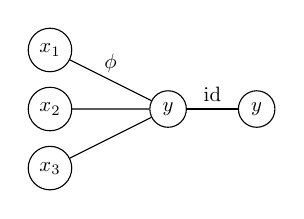
\begin{tikzpicture}[node distance=1.5cm, every node/.style={scale=0.75}, scale=0.75]

% Input layer
\foreach \i in {1,2,...,3}
	\node[circle, draw=black, minimum size=0.5cm] (x\i) at (0,4-\i) {$x_\i$};
	
% Hidden layer 
\node[circle, draw=black, minimum size=0.5cm] (y) at (2,2) {$y$};

% Output layer
\node[circle, draw=black, minimum size=0.5cm] (y2) at (3.5,2) {$y$};

% Connections from input to hidden layer
\foreach \i in {1,2,...,3}
	\draw (x\i) -- (y);
\path (x1) -- node[midway,above] {$\phi$} (y);

% Connections from hidden to output layer
\draw (y) -- node[midway,above] {$\text{id}$} (y2);
\end{tikzpicture}
\hspace{1cm}
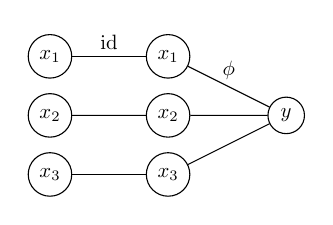
\begin{tikzpicture}[node distance=1.5cm, every node/.style={scale=0.75}, scale=0.75]

% Input layer
\foreach \i in {1,2,...,3}
	\node[circle, draw=black, minimum size=0.5cm] (x\i) at (0,4-\i) {$x_\i$};

% Hidden layer
\foreach \i in {1,2,...,3}
	\node[circle, draw=black, minimum size=0.5cm] (h\i) at (2,4-\i) {$x_\i$};

% Output layer
\node[circle, draw=black, minimum size=0.5cm] (y) at (4,2) {$y$};

% Connections from input to hidden layer
\foreach \i in {1,2,...,3}
	\draw (x\i) -- (h\i);
 \path (x1) -- node[midway,above] {$\text{id}$} (h1);

% Connections from hidden to output layer
\foreach \i in {1,2,...,3}
	\draw (h\i) -- (y);
 \path (h1) -- node[midway,above] {$\phi$} (y);
\end{tikzpicture}
\captionof{figure}{Left: Instance of a two-layer NN embedding the NLRM in the first layer. Right: Instance of a two-layer NN embedding the NLRM in the second layer.}
\label{fig:NLRM2}
\end{figure}

\subsection{Spectrum of the Second-Layer Hessian with Weights}\label{sec:main-IIW}
Of course, the assumption $W^{(1)}=I_d$ is too restrictive, as it prevents us from training the model. Therefore, we attempt to derive a result for arbitrary (but fixed) $W^{(1)}\in\mathbb{R}^{d\times d}$, again by using the Bai-Silverstein method. For general $W^{(1)}$, the main technical issue is use a concentration argument for quadratic forms with dependencies. We will need to apply the concentration inequality for $x^\top A x$ with $x=\tilde{x}_\ell=\phi(W^{(1)}x_\ell)$, and
\begin{equation}
A=Q_d^{-\ell}(z)=\left(-zI_d + \frac{1}{n}\sum_{\substack{k=1 \\ k\neq\ell}}^n\phi(W^{(1)}x_k)\phi(W^{(1)}x_k)^\top\right)^{-1}.
\end{equation}
Its expectation is computed as follows:
\begin{align}
\mathbb{E}_{x}[\phi(W^{(1)}x_\ell)^\top A\, \phi(W^{(1)}x_\ell)] &= \sum_{i,j=1}^d A_{ij}\underbrace{\mathbb{E}_{x}[\phi(W^{(1)}x_\ell)_i\,\phi(W^{(1)}x_\ell)_j]}_{=:\Sigma_\phi(W^{(1)})_{ij}} = \operatorname{Tr}(\Sigma_\phi(W^{(1)})A).
\end{align}
This motivates the following definition, which can be thought of as a generalization of the parameter $\sigma_\phi^2=\mathbb{E}[\phi(x_1)^2]$, present in the previous case $W^{(1)}=I_d$.
\bigskip
\begin{definition}[Auxiliary Covariance Matrix] Define the matrix $\Sigma_\phi(W^{(1)})\in\mathbb{R}^{d\times d}$ (for fixed $W^{(1)}$) via
\begin{equation*}
\Sigma_\phi(W^{(1)})_{ij}:=\mathbb{E}_x\left[\phi(W^{(1)}x)_i\,\phi(W^{(1)}x)_j\right]=\mathbb{E}_x\left[\phi\left(\sum_{k=1}^dW^{(1)}_{i,k}x_k\right)\phi\left(\sum_{k=1}^dW^{(1)}_{j,k}x_k\right)\right].
\end{equation*} \label{def:SigmaW}
\end{definition}
\bigskip
\par
The key assumption required for the Bai-Silverstein analysis, in the context of the two-layer network, is that the operator norm of the auxiliary matrix above is bounded as $d\to\infty$.
\bigskip
\begin{assumption}[Optimal Scaling Assumption on $W^{(1)}$]
Let $\Sigma_\phi(W^{(1)})\in\mathbb{R}^{d\times d}$ be as in Definition \ref{def:SigmaW}. Then, there exists a function $f_\phi:\mathbb{R}\to\mathbb{R}$ such that $k\geq0$ is minimal with
$$\|\Sigma_\phi(W^{(1)})\|\,\leq\mathcal{O}(1) \quad\text{and}\quad W^{(1)}_{ij}=\frac{1}{f_\phi(d)}\tilde{W}_{ij}=\mathcal{O}(d^{-k}),\quad \tilde{W}_{ij}=\mathcal{O}(1),$$\label{ass:scaling-W}
almost surely as $d\to\infty$.
\end{assumption}
\bigskip
\par
The assumption above emphasizes that the scaling of $W^{(1)}$ is chosen to be optimal such that the bound $\|\Sigma_\phi(W^{(1)})\|\,\leq\mathcal{O}(1)$ is satisfied.
\bigskip
\par
In order to handle the dependencies in (\ref{eq:linearcombination}) between the entries of $\tilde{x}_\ell=\phi(W^{(1)}x_\ell)$, we exploit Lemma 1 in \cite{louart}.
\bigskip
\begin{lemma}
Assume that $\phi:\mathbb{R}\to\mathbb{R}$ is $L_\phi$-Lipschitz continuous with $L_\phi>0$, and $x\sim\mathcal{N}(0,I_d)$ a normal random vector. Define $\tilde{x}:=\phi(W^{(1)}x)$, where $W^{(1)}\in\mathbb{R}^{d\times d}$ is arbitrary with Assumption \ref{ass:scaling-W}. Then, for any matrix $A\in\mathbb{R}^{d\times d}$ with $\|A\|\,\leq\mathcal{O}(1)$ as $d\to\infty$, there exist $C,c>0$ (independent of $d$) such that for all $t\geq0$
$$P\left(\left|\frac{1}{d}\tilde{x}^\top A \tilde{x}-\frac{1}{d}\operatorname{Tr}\left(\Sigma_\phi(W^{(1)})A\right)\right|\geq t\right)\leq C\exp\left(-\frac{c\,d}{\|W^{(1)}\|^2L_\phi^2}\min\left\{\frac{t^2}{t_0^2},t^2\right\}\right),$$
where $t_0=|\phi(0)|+L_\phi\|W^{(1)}\|\sqrt{n/d}=\mathcal{O}(1)$.\label{thm:louart}
\end{lemma}
\bigskip
\par
Combining the concentration inequality above with the elementary fact that 
\\$\mathbb{E}[|Z|]=\int_0^\infty P(|Z|>t)\,dt$ for all random variables $Z$, one obtains the following result, which is also found in Corollary 1 of Louart et al. \cite{louart}.
\bigskip
\begin{corollary}[Trace Concentration with Dependence] Assume that $\phi:\mathbb{R}\to\mathbb{R}$ is $L_\phi$-Lipschitz continuous with $L_\phi>0$, and $x\sim\mathcal{N}(0,I_d)$ a normal random vector. Define $\tilde{x}:=\phi(W^{(1)}x)$, where $W^{(1)}\in\mathbb{R}^{d\times d}$ is arbitrary with Assumption \ref{ass:scaling-W}. Then, for any matrix $A\in\mathbb{R}^{d\times d}$ with $\|A\|\,\leq\mathcal{O}(1)$ as $d\to\infty$,
\begin{equation*}
\mathbb{E}\left[\left(\frac{1}{d}\tilde{x}^\top A \tilde{x}-\frac{1}{d}\operatorname{Tr}\left(\Sigma_\phi(W^{(1)})A\right)\right)^4\right]\leq\mathcal{O}(d^{-2}),
\end{equation*}
as $d\to\infty$, which consequently yields, almost surely as $d\to\infty$,
$$\frac{1}{d}\tilde{x}^\top A\tilde{x}\simeq\frac{1}{d}\operatorname{Tr}\left(\Sigma_\phi(W^{(1)})A\right).$$\label{thm:trace-lemma2}
\end{corollary}
\bigskip
\par
We remind the reader that we omit detailed computations and explanations of the steps in the Proof of our following main result, due to its similarity with the proof of Theorem \ref{thm:mainresult-1}. Therefore, we strongly suggest to read the proof of Theorem \ref{thm:mainresult-1} first.
\bigskip
\begin{theorem}[Main Result II with Weights]
Let $X=[x_1,\dots,x_n]\in\mathbb{R}^{d\times n}$ have i.i.d. entries $X_{ij}\sim\mathcal{N}(0,1)$, and $W^{(1)}\in\mathbb{R}^{d\times d}$ satisfy Assumption \ref{ass:scaling-W}, respectively. Let $Q_d(z)$ be the resolvent of $H_2$, and assume that $n/d\to\alpha\in(1,\infty)$ as $n,d\to\infty$. Furthermore, assume that $\phi:\mathbb{R}\to\mathbb{R}$ is Lipschitz continuous. Then the Stieltjes transform $m_{H_2}(z)$ satisfies, for all $z\in\mathbb{C}_+$ almost surely as $n,d\to\infty$, that
\begin{equation*}
m_{H_2}(z)\simeq\frac{1}{d}\operatorname{Tr}\left(\frac{\Sigma_\phi(W^{(1)})}{1+\alpha^{-1}\delta_d(z)}-zI_d\right)^{-1},
\end{equation*}
where $\delta_d:\mathbb{C}_+\to\mathbb{R}$ is given by the fixed point equation
\begin{equation}
\delta_d(z)=\frac{1}{d}\operatorname{Tr}\left(\Sigma_\phi(W^{(1)})\left(\frac{\Sigma_\phi(W^{(1)})}{1+\alpha^{-1}\delta_d(z)}-zI_d\right)^{-1}\right).
\end{equation} \label{thm:mainresult-2W}
\end{theorem}
\bigskip
In this result, the fixed point equation is now not in the Stieltjes transform $m_{H_2}(z)$, but rather in the newly introduced parameter $\delta_d(z)$, required for the direct evaluation of $m_{H_2}(z)$. Moreover, Theorem \ref{thm:mainresult-2W} yields the same formula as in Theorem 2 of Louart et al. \cite{louart}. The main difference is in the definition of $\Sigma_\phi(W^{(1)})$, where we take the expectation over the data $x$ instead over the weights.
\bigskip
\\
\emph{Proof.} Let $z\in\mathbb{C}_+$ and $W^{(1)}\in\mathbb{R}^{d\times d}$ be arbitrary as in Assumption \ref{ass:scaling-W}. We write
\begin{equation}
H_2(W^{(1)})=\frac{1}{n}\sum_{\ell=1}^n\phi(W^{(1)}x_\ell)\phi(W^{(1)}x_\ell)^\top=\frac{1}{n}\sum_{\ell=1}^n\tilde{x}_\ell\tilde{x}_\ell^\top\in\mathbb{R}^{d\times d},
\end{equation}
with the random vectors $\tilde{x}_\ell:=\phi(W^{(1)}x_\ell)\in\mathbb{R}^{d}$. Let $z\in\mathbb{C}_+$ be arbitrary. By Assumption \ref{ass:key-assumption}, we know that the limiting Stieltjes transform $m_{H_2}(z)$ is determined by
$$\frac{1}{d}\operatorname{Tr}Q_d(z)\stackrel{a.s.}{\to}m_{H_2}(z),$$
as $d\to\infty$. Therefore, it is a well-defined problem trying to find a solution $\overline{Q_d}(z)\in\mathbb{R}^{d\times d}$ of
\begin{align}
\frac{1}{d}\operatorname{Tr}Q_{d}(z)&\simeq\frac{1}{d}\operatorname{Tr}\overline{Q_{d}}(z),\quad\|\overline{Q_d}(z)\|\,\leq\mathcal{O}(1),\quad\text{almost surely as $d\to\infty$,} \label{eq:deterministic-equivalent2}
\\ &\quad\text{and define}\quad \delta_d(z):=\frac{1}{d}\operatorname{Tr}\left(\Sigma_\phi(W^{(1)})\overline{Q_d}(z)\right). \notag
\end{align}
By the resolvent identity, Lemma \ref{thm:resolvent}, we have
\begin{align}
Q_{d}(z)-\overline{Q_{d}}(z) &= Q_{d}(z)\left(\overline{Q_{d}}(z)^{-1}-Q_{d}(z)^{-1}\right)\overline{Q_{d}}(z) \notag
\\ &= Q_{d}(z)\left(\overline{Q_{d}}(z)^{-1}+zI_{d}-\frac{1}{n}\sum_{\ell=1}^n\tilde{x_\ell}\tilde{x_\ell}^\top\right)\overline{Q_{d}}(z).
\end{align}
Therefore, almost surely as $d\to\infty$, using (\ref{eq:deterministic-equivalent2}) and the cyclic property of the trace operator,
\begin{align}
0&\simeq\frac{1}{d}\operatorname{Tr}\left(Q_d(z)-\overline{Q_d}(z)\right) =\frac{1}{d}\operatorname{Tr}\left(Q_{d}(z)\left(\overline{Q_{d}}(z)^{-1}+zI_{d}-\frac{1}{n}\sum_{\ell=1}^n\tilde{x_\ell}\tilde{x_\ell}^\top\right)\overline{Q_{d}}(z)\right) \notag
\\&= \frac{1}{d}\operatorname{Tr}\left(\left(\overline{Q_{d}}(z)^{-1}+zI_{d}-\frac{1}{n}\sum_{\ell=1}^n\tilde{x_\ell}\tilde{x_\ell}^\top\right)\overline{Q_{d}}(z)Q_{d}(z)\right) \notag
\\&= \frac{1}{d}\operatorname{Tr}\left((zI_{d}+\overline{Q_{d}}(z)^{-1})\overline{Q_{d}}(z)Q_{d}(z)\right)-\frac{1}{dn}\sum_{\ell=1}^n\operatorname{Tr}\left(\tilde{x_\ell}\tilde{x_\ell}^\top\overline{Q_d}(z)Q_d(z)\right).
\end{align}
A quadratic form emerges from the trivial relationship
\begin{equation}
\operatorname{Tr}(\tilde{x}_\ell \tilde{x}_\ell^\top\overline{Q_d}(z)Q_d(z)) =\tilde{x}_\ell^\top\overline{Q_d}(z)Q_d(z)\tilde{x}_\ell,
\end{equation}
implying that
\begin{equation}
\frac{1}{d}\operatorname{Tr}\left((zI_{d}+\overline{Q_{d}}(z)^{-1})\overline{Q_{d}}(z)Q_{d}(z)\right)\simeq \frac{1}{dn}\sum_{\ell=1}^n \tilde{x_\ell}^\top\overline{Q_{d}}(z)Q_{d}(z)\tilde{x_\ell}.\label{eq:trace-sim2c}
\end{equation}
We continue by rewriting (\ref{eq:trace-sim2c}) as
\begin{align}
\frac{1}{dn}&\sum_{\ell=1}^n \tilde{x}_\ell^\top\overline{Q_{d}}(z)Q_{d}(z)\tilde{x}_\ell = \frac{1}{dn}\sum_{\ell=1}^n \tilde{x}_\ell^\top\overline{Q_{d}}(z)\left(-zI_{d}+\frac{1}{n}\sum_{k=1}^n \tilde{x}_k \tilde{x}_k^\top\right)^{-1}\tilde{x}_\ell \notag
\\&= \frac{1}{dn}\sum_{\ell=1}^n \tilde{x}_\ell^\top\overline{Q_{d}}(z)\left(-zI_{d}+\frac{1}{n}\sum_{\substack{k=1 \\ k\neq\ell}}^n \tilde{x}_k\tilde{x}_k^\top+\frac{1}{n} \tilde{x}_\ell \tilde{x}_\ell^\top\right)^{-1}\tilde{x}_\ell.
\end{align}
Now, we wish to make use of Sherman-Morrison, Lemma \ref{thm:SM}, and consider the "leave-one-out"-modification
\begin{equation}
Q_{d}^{-\ell}(z):=\left(-zI_{d} + \frac{1}{n}\sum_{\substack{k=1 \\ k\neq\ell}}^n \tilde{x}_k\tilde{x}_k^\top\right)^{-1}=\left(-zI_d + \frac{1}{n}\sum_{\substack{k=1 \\ k\neq\ell}}^n\phi(W^{(1)}x_k)\phi(W^{(1)}x_k)^\top\right)^{-1}
\end{equation}
of the resolvent $Q_{d}(z)$ which differs by the rank-1 perturbation $\frac{1}{n}\tilde{x}_\ell \tilde{x}_\ell^\top$. Moreover, since we fixed $W^{(1)}$ and only consider the expectation with respect to the distribution of the $x_\ell$ (not $\tilde{x}_\ell$), the matrix $Q_{d}^{-\ell}(z)$ is clearly independent of $\tilde{x}_\ell$. We apply Lemma \ref{thm:SM} with $u=\tilde{x}_\ell$, $v=\frac{1}{n}\tilde{x}_\ell$ and $A=-zI_{d}+\frac{1}{n}\sum\limits_{k\neq\ell}\tilde{x}_k\tilde{x}_k^\top$ (i.e. $A^{-1}=Q_{d}^{-\ell}(z)$), leading to the identity
\begin{equation}
Q_{d}(z)\tilde{x}_\ell = \frac{Q_{d}^{-\ell}(z)\tilde{x}_\ell}{1+\frac{1}{n}\tilde{x}_\ell^\top Q_{d}^{-\ell}(z)\tilde{x}_\ell}
\end{equation}
Next, we concentrate the quadratic form in the denominator by applying Corollary \ref{thm:trace-lemma2} to the random vector $\tilde{x}_\ell=\phi(W^{(1)}x_\ell)$ recalling its independence of the matrix $Q_{d}^{-\ell}(z)$.
\bigskip
\par
Therefore, we have
 \begin{align}
\frac{1}{dn}&\sum_{\ell=1}^n \tilde{x}_\ell^\top\overline{Q_{d}}(z)\cdot Q_{d}(z)\tilde{x}_\ell = \frac{1}{dn}\sum_{\ell=1}^n \tilde{x}_\ell^\top\overline{Q_{d}}(z)\cdot \frac{Q_{d}^{-\ell}(z)\tilde{x}_\ell}{1+\frac{1}{n}\tilde{x}_\ell^\top Q_{d}^{-\ell}(z)\tilde{x}_\ell} \notag
\\ &= \frac{1}{n}\sum_{\ell=1}^n\frac{1}{1+\frac{1}{n}\tilde{x}_\ell^\top Q_{d}^{-\ell}(z)\tilde{x}_\ell}\cdot\frac{1}{d}\tilde{x}_\ell^\top\overline{Q_{d}}(z)Q_{d}^{-\ell}(z)\tilde{x}_\ell \notag
\\ &\simeq \frac{1}{n}\sum_{\ell=1}^n\frac{1}{1+\alpha^{-1}\delta_d(z)}\cdot\frac{1}{d}\tilde{x}_\ell^\top\overline{Q_{d}}(z)Q_{d}^{-\ell}(z)\tilde{x}_\ell \label{eq:BS-argument1-II}
\\ &= \frac{1}{1+\alpha^{-1}\delta_d(z)}\cdot\frac{1}{n}\sum_{\ell=1}^n\frac{1}{d}\tilde{x}_\ell^\top\overline{Q_{d}}(z)Q_{d}^{-\ell}(z)\tilde{x}_\ell \notag
\\ &\simeq \frac{1}{1+\alpha^{-1}\delta_d(z)}\left(\frac{1}{d}\operatorname{Tr}\left(\Sigma_\phi(W^{(1)})\overline{Q_{d}}(z)Q_{d}(z)\right)\right) \label{eq:BS-argument2-II}
\\ &= \frac{1}{d}\operatorname{Tr}\left(\frac{1}{1+\alpha^{-1}\delta_d(z)}\Sigma_\phi(W^{(1)})\overline{Q_{d}}(z)Q_{d}(z)\right). \notag
\end{align}
The equivalence in (\ref{eq:BS-argument1-II}) above is derived by using Lemma \ref{thm:rank-1-perturbation} and Corollary \ref{thm:trace-lemma2} as follows:
\begin{align}
\frac{1}{n}\tilde{x}_\ell^\top Q_{d}^{-\ell}(z)\tilde{x}_\ell &= \frac{d}{n}\frac{1}{d}\tilde{x}_\ell^\top Q_{d}^{-\ell}(z)\tilde{x}_\ell \simeq \alpha^{-1}\frac{1}{d}\tilde{x}_\ell^\top Q_{d}^{-\ell}(z)\tilde{x}_\ell \notag
\\ &\stackrel{\ref{thm:trace-lemma2}}{\simeq} \alpha^{-1}\frac{1}{d}\operatorname{Tr}\left(\Sigma_\phi(W^{(1)})Q_d^{-\ell}(z)\right) \notag
\\ &\stackrel{\ref{thm:rank-1-perturbation}}{\simeq} \alpha^{-1}\frac{1}{d}\operatorname{Tr}\left(\Sigma_\phi(W^{(1)})Q_d(z)\right) \notag
\\ &\simeq\alpha^{-1}\frac{1}{d}\operatorname{Tr}\left(\Sigma_\phi(W^{(1)})\overline{Q_d}(z)\right)=\alpha^{-1}\delta_d(z)\label{eq:lemmaW1}
\end{align}
for all $\ell=1,\dots,n$, almost surely as $n,d\to\infty$. Note that we also used $n/d\to\alpha$, and, in the last line above, (\ref{eq:deterministic-equivalent2}) paired with the condition $\|\Sigma_\phi(W^{(1)})\|\,\leq\mathcal{O}(1)$, as $d\to\infty$,
\begin{align}
\frac{1}{d}\operatorname{Tr}\left(\Sigma_\phi(W^{(1)})(Q_d(z)-\overline{Q_d}(z))\right)\leq\underbrace{\|\Sigma_\phi(W^{(1)})\|}_{\leq\mathcal{O}(1)}\cdot\underbrace{\frac{1}{d}\operatorname{Tr}\left(Q_d(z)-\overline{Q_d}(z)\right)}_{\to0}\to0.
\end{align}
\par
In a similar manner, we obtain the equivalence in (\ref{eq:BS-argument2-II}) from
\begin{align}
\frac{1}{d}&\tilde{x}_\ell^\top\overline{Q_{d}}(z)Q_{d}^{-\ell}(z)\tilde{x}_\ell \notag
\\ &\stackrel{\ref{thm:trace-lemma2}}{\simeq} \frac{1}{d}\operatorname{Tr}\left(\Sigma_\phi(W^{(1)})\overline{Q_{d}}(z)Q_{d}^{-\ell}(z)\right) \notag
\\ &\stackrel{\ref{thm:rank-1-perturbation}}{\simeq} \frac{1}{d}\operatorname{Tr}\left(\Sigma_\phi(W^{(1)})\overline{Q_{d}}(z)Q_{d}(z)\right)\label{eq:lemmaW2}
\end{align}
for all $\ell=1,\dots,n$, almost surely as $n,d\to\infty$.
\bigskip
\par
Note that in (\ref{eq:lemmaW1}) and (\ref{eq:lemmaW2}), we applied Lemma \ref{thm:rank-1-perturbation} to 
\\ $A\in\{\Sigma_\phi(W^{(1)}),\Sigma_\phi(W^{(1)})\overline{Q_d}(z)\}$, which requires $\|A\|\leq\mathcal{O}(1)$. The bound indeed holds true since
\begin{equation}
\|A\|\,=\|\Sigma_\phi(W^{(1)})B\|\,\leq\underbrace{\|\Sigma_\phi(W^{(1)})\|}_{\leq\mathcal{O}(1)}\cdot\,\|B\|\,\leq\mathcal{O}(1)
\end{equation}
for $B\in\{I_d,\overline{Q_d}(z)\}$, where we already justified $\|B\|\,\leq\mathcal{O}(1)$ in the proof of Theorem \ref{thm:mainresult-1}.
\par
Similarly, we also used Corollary \ref{thm:trace-lemma2} 
 in (\ref{eq:lemmaW1}) and (\ref{eq:lemmaW2}), with 
 \\ $A\in\{Q_d^{-\ell}(z), \overline{Q_d}(z)Q_d^{-\ell}(z)\}$, which requires that $\|A\|\,\leq\mathcal{O}(1)$. It been shown at the end of the proof of Theorem \ref{thm:mainresult-1} that $\|Q_d^{-\ell}(z)\|\,\leq\mathcal{O}(1)$, from which the desired bound follows by submultiplicativity of $\|\cdot\|$.
\bigskip
\par
In summary, combining (\ref{eq:trace-sim2c}) and (\ref{eq:BS-argument2-II}), this leaves us with
\begin{align}
\frac{1}{d}&\operatorname{Tr}\left((zI_{d}+\overline{Q_{d}}(z)^{-1})\overline{Q_{d}}(z)Q_{d}(z)\right) \simeq \frac{1}{dn}\sum_{\ell=1}^n \tilde{x}_\ell^\top\overline{Q_{d}}(z)Q_{d}(z)\tilde{x}_\ell \notag
\\ &\simeq \frac{1}{d}\operatorname{Tr}\left(\frac{1}{1+\alpha^{-1}\delta_d(z)}\Sigma_\phi(W^{(1)})\overline{Q_{d}}(z)Q_{d}(z)\right)\label{eq:Q-identity2}
\end{align}
almost surely as $n,d\to\infty$. Therefore, we may establish
\begin{equation}
zI_{d}+\overline{Q_{d}}(z)^{-1}\stackrel{!}{=}\frac{1}{1+\alpha^{-1}\delta_d(z)}\Sigma_\phi(W^{(1)})
\end{equation}
such that (\ref{eq:Q-identity2}) is satisfied, allowing us to finally determine $\overline{Q_d}(z)\in\mathbb{R}^{d\times d}$. That is, we can take
\begin{equation}
\overline{Q_{d}}(z):=\left(\frac{\Sigma_\phi(W^{(1)})}{1+\alpha^{-1}\delta_d(z)}-zI_{d}\right)^{-1}
\end{equation}
for (\ref{eq:deterministic-equivalent2}) to hold true, almost surely as $n,d\to\infty$. We will show at the end that indeed $\|\overline{Q_d}(z)\|\,\leq\mathcal{O}(1)$. We conclude that, almost surely as $n,d\to\infty$,
\begin{align}
m_{H_2}(z) &\simeq\frac{1}{d}\operatorname{Tr}Q_{d}(z) \simeq\frac{1}{d}\operatorname{Tr}\overline{Q_{d}}(z) = \frac{1}{d}\operatorname{Tr}\left(\frac{\Sigma_\phi(W^{(1)})}{1+\alpha^{-1}\delta_d(z)}-zI_{d}\right)^{-1}
\end{align}
and by (\ref{eq:deterministic-equivalent2}) we have the desired fixed point equation
\begin{equation}
\delta_d(z)=\frac{1}{d}\operatorname{Tr}\left(\Sigma_\phi(W^{(1)})\overline{Q_d}(z)\right)=\frac{1}{d}\operatorname{Tr}\left(\Sigma_\phi(W^{(1)})\left(\frac{\Sigma_\phi(W^{(1)})}{1+\alpha^{-1}\delta_d(z)}-zI_{d}\right)^{-1}\right).
\end{equation}
It remains to show that indeed $\|\overline{Q_d}(z)\|\,\leq\mathcal{O}(1)$. First, observe that
\begin{align}
\delta_d(z) &= \frac{1}{d}\operatorname{Tr}\left(\Sigma_\phi(W^{(1)})\overline{Q_d}(z)\right)\leq\|\Sigma_\phi(W^{(1)})\|\,\frac{1}{d}\operatorname{Tr}\overline{Q_d}(z) \notag
\\ &\stackrel{(\ref{eq:deterministic-equivalent2})}{\simeq} \|\Sigma_\phi(W^{(1)})\|\,\frac{1}{d}\operatorname{Tr}Q_d(z)\simeq\|\Sigma_\phi(W^{(1)})\|\, m_{H_2}(z).
\end{align}
Thererfore,
\begin{align}
\left\|\overline{Q_d}(z)\right\| &= \left\|\left(\frac{\Sigma_\phi(W^{(1)})}{1+\alpha^{-1}\delta_d(z)}-zI_{d}\right)^{-1}\right\| \notag
\\ &\leq \left\|\left(\frac{\Sigma_\phi(W^{(1)})}{1+\alpha^{-1}m_{H_2}(z)\left\|\Sigma_\phi(W^{(1)})\right\|}-zI_{d}\right)^{-1}\right\|\leq\mathcal{O}(1),
\end{align}
which concludes the proof.
\qed
\bigskip
\bigskip
\\
\textbf{Scaling Assumption on $W^{(1)}$.} In practice, one usually considers scaling conditions of the form $W^{(1)}=d^{-1/2}\tilde{W}$ with $\tilde{W}$ having entries of order $\mathcal{O}(1)$. This is important for avoiding the vanishing gradient problem \cite{orvieto}. If $\phi=\operatorname{id}$, and if $\tilde{W}$ is randomly initialized with i.i.d. normal entries (independent of $X$), then the Marchenko-Pastur law implies that the limiting spectral distribution of
\begin{equation}
\Sigma_{\operatorname{id}}(W^{(1)})=\mathbb{E}_{x}[W^{(1)} x x^\top {W^{(1)}}^\top]=\frac{1}{d}\tilde{W}\tilde{W}^\top
\end{equation}
has bounded support, recalling from Assumption \ref{ass:data} that $x_\ell$ has unit covariance, 
\\ $\mathbb{E}[x_\ell x_\ell^\top]=I_d$. But this does not necessarily imply $\|\Sigma_{\operatorname{id}}(W^{(1)})\|\,\leq\mathcal{O}(1)$. To our convenience, we can exploit Theorem 2.3.23 in \cite{tao} to deduce that indeed $\left\|\Sigma_{\operatorname{id}}(W^{(1)})\right\|\leq\mathcal{O}(1)$. A small technical detail worth mentioning is that Theorem 2.3.23 in \cite{tao} requires that $\tilde{W}$ is symmetric. However, we may bypass this condition by applying the theorem to the symmetric matrix
\begin{equation}
\begin{bmatrix} 0 & \tilde{W} \\ \tilde{W}^\top & 0, \end{bmatrix}
\end{equation}
which has the same operator norm as $\|\tilde{W}\|$.
\par
We will now show that it is, in principle, possible to ensure the necessary bound $\|\Sigma_\phi(W^{(1)})\|\,\leq\mathcal{O}(1)$ for arbitrary activations $\phi$. However, the following strategy does not provide an optimal solution in the sense of Assumption \ref{ass:scaling-W}. Recall from Definition \ref{def:SigmaW} that
\begin{equation}
\Sigma_\phi(W^{(1)})_{ij}=\mathbb{E}_x\left[\phi\left(\sum_{k=1}^dW^{(1)}_{i,k}x_k\right)\phi\left(\sum_{k=1}^dW^{(1)}_{j,k}x_k\right)\right].
\end{equation}
Let $f_\phi:\mathbb{R}\to\mathbb{R}$ be a function such that \begin{equation}
\phi(f_\phi(d)\,d)\leq\mathcal{O}(d^{-1/2})\quad\text{as}\quad d\to\infty.\label{eq:scaling}
\end{equation}
If we assume that $W^{(1)}_{ij}=f_\phi(d)\tilde{W}_{ij}$ for entries $\tilde{W}_{ij}=\mathcal{O}(1)$, then $x_i=\mathcal{O}(1)$ implies $\sum_{k=1}^d\tilde{W}_{i,k}x_k=\mathcal{O}(d)$ for all $i=1,\dots,d$. Therefore, by using (\ref{eq:scaling}),
\begin{align}
\|\Sigma_\phi(W^{(1)})\|\,&\leq\operatorname{Tr}\Sigma_\phi(W^{(1)})=\sum_{i=1}^d\Sigma_\phi(W^{(1)})_{ii} = \mathbb{E}_x\left[\sum_{i=1}^d\phi\left(\sum_{k=1}^dW^{(1)}_{i,k}x_k\right)^2\right]
\\ &= \mathbb{E}_x\Biggl[\sum_{i=1}^d\underbrace{\phi\left(f_\phi(d)\sum_{k=1}^d\tilde{W}_{i,k}x_k\right)^2}_{\leq\mathcal{O}(d^{-1})}\,\Biggr]\leq\mathcal{O}(1).
\end{align}
\par
Following this logic with $\phi=\operatorname{id}$, (\ref{eq:scaling}) yields that $f_\phi(d)\leq\mathcal{O}(d^{-3/2})$, which is indeed suboptimal compared to the previous discussion where we were able to achieve $f_\phi(d)=\mathcal{O}(d^{-1/2})$ using Theorem 2.3.23 in \cite{tao}.
\bigskip
\bigskip
\\
\textbf{Consistency with Theorem \ref{thm:mainresult-2}.} It is worth mentioning that we obtain Theorem \ref{thm:mainresult-2} as a special case of Theorem \ref{thm:mainresult-2W} when using it with $W^{(1)}=I_d$. Indeed, $W^{(1)}=I_d$ yields 
\begin{equation}
\Sigma_\phi(I_d)_{ij}=\mathbb{E}_x[\phi(x)_i\phi(x)_j]\delta_{ij}=\mathbb{E}_x[\phi(x_1)^2]\delta_{ij}=\sigma_\phi^2\delta_{ij},
\end{equation}
recalling from Assumption \ref{ass:data} that $x_\ell$ has unit covariance, $\mathbb{E}[x_\ell x_\ell^\top]=I_d$. Thus, $\Sigma_\phi(I_d)=\sigma_\phi^2 I_d$. Theorem \ref{thm:mainresult-2W} states that the Stieltjes transform $m_{H_2}(z)$ satisfies, for all $z\in\mathbb{C}_+$ as $n,d\to\infty$, that
\begin{align}
m_{H_2}(z) &\simeq \frac{1}{d}\operatorname{Tr}\left(\frac{\Sigma_\phi(I_d)}{1+\alpha^{-1}\delta_d(z)}-zI_d\right)^{-1}\simeq\frac{1}{d}\operatorname{Tr}\left(\frac{\sigma_\phi^2I_d}{1+\alpha^{-1}\sigma_\phi^2\,m_{H_2}(z)}-zI_d\right)^{-1} \notag
\\&= \left(\frac{\sigma_\phi^2}{1+\alpha^{-1}\sigma_\phi^2\,m_{H_2}(z)}-zI_d\right)^{-1},
\end{align}
where we used
\begin{align}
\delta_d(z) &= \frac{1}{d}\operatorname{Tr}\left(\Sigma_\phi(I_d)\left(\frac{\Sigma_\phi(I_d)}{1+\alpha^{-1}\delta_d(z)}-zI_d\right)^{-1}\right) \notag
\\&= \frac{\sigma_\phi^2}{d}\operatorname{Tr}\left(\frac{\Sigma_\phi(I_d)}{1+\alpha^{-1}\delta_d(z)}-zI_d\right)^{-1}\simeq\sigma_\phi^2 \,m_{H_2}(z).
\end{align}
\bigskip
\bigskip
\\
\textbf{The Problem with Numerical Simulations if $W^{(1)}\neq I_d$.} Unfortunately, we encounter similar difficulties with numerical experiments as in the discussion about the non-zero-mean case $\mu_\phi\neq0$, following Theorem \ref{thm:mainresult-2}. Namely, we have to compute the inverse
\begin{equation}
\left(\frac{\Sigma_\phi(W^{(1)})}{1+\alpha^{-1}\delta_d(z)}-zI_d\right)^{-1},\label{eq:inverse}
\end{equation}
which is expensive for large $d$, especially if we need it for many iterations in $z$. Of course, if $W^{(1)}=I_d$, then $\Sigma_\phi(W^{(1)})=\sigma_\phi^2I_d$, making the computations much easier. The same is true for the parameter $\delta_d(z)$, which also involves the computation of (\ref{eq:inverse}).

\subsection{Spectral Dynamics of the Second-Layer Hessian}
Proceeding similarly as in Section \ref{sec:training}, we can generalize Theorem \ref{thm:mainresult-2W} such that it respects the training of the model. Recalling the vecorization
\begin{equation}
\theta=(\theta_1,\dots,\theta_{(d+m)d})^\top:=(\vec{w}_1^\top,\vec{w}_2^\top)^\top\in\mathbb{R}^{(d+m)d}
\end{equation}
of the trainable parameters $W^{(1)}$ and $W^{(2)}$, we formulate the gradient method
\begin{equation}
\frac{\partial \theta_t}{\partial t} = \theta_t-M_t\nabla_w\mathcal{L}(\theta_t),\quad \theta_{t=0}=\theta_0.\label{eq:gradientflow2}
\end{equation}
Just like before, the matrix $M_t\in\mathbb{R}^{d\times d}$ For example: $M_t=\eta_tI_d$ (standard GD), $M_t=\mathcal{H}(w_t)^{-1}$ (second-order GD), and $M_t=F(w_t)^{-1}$ (natural GD), where the matrix
$F(w_t):=\mathbb{E}\left[(\nabla_w\log \mathcal{L}(w_t))(\nabla_w\log \mathcal{L}(w_t))^\top \right]$ denotes the Fisher information matrix.
\smallskip
\par
In our two-layer model, the gradient elements of the loss are given by
\begin{align}
\frac{\partial\mathcal{L}(\theta)}{\partial \theta_k} &= \frac{1}{n}\sum_{i=1}^n\sum_{j=1}^m((f_\theta^{(2)}(x_i))_j-(y_i)_j)\cdot\frac{\partial}{\partial\theta_k}(f_\theta^{(2)}(x_i)),
\end{align}
where $f_\theta^{(2)}(x)=({W^{(2)}} \phi({W^{(1)}} x))$, and
\begin{equation}
\frac{\partial}{\partial\theta_k}(f_\theta^{(2)}(x_i))_j = \begin{cases}  \phi\left((W^{(1)}x_i)_{k_1}\right)\cdot\delta_{k_2j}, & \theta_k=W_{k_2k_1}^{(2)}\\
W_{jk_1}^{(2)}\phi'\left((W^{(1)}x_i)_{k_1}\right)\cdot (x_i)_{k_0}, & \theta_k=W_{k_1k_0}^{(1)}\end{cases}
\end{equation}
as shown in Appendix \ref{sec:appendix_proof}.
\smallskip
\par
The exact solution of the gradient flow equation (\ref{eq:gradientflow2}) is obtained from the fundamental theorem of calculus:
\begin{equation}
\theta_t=\theta_0-\int_0^t M_s\nabla_\theta\mathcal{L}(\theta_s)\,ds.\label{eq:GD2}
\end{equation}
Having the variational parameters $\theta_t\in\mathbb{R}^{(d+m)d}$ at each time $t\geq0$ at our disposal, we can simply obtain the time-evolution of the Hessian via
\begin{equation}
H_2(t)\equiv H_2(W^{(1)}_t)=I_m\otimes\frac{1}{n}\sum_{\ell=1}^n\phi(W^{(1)}_tx_\ell)\phi(W^{(1)}_tx_\ell)^\top\in\mathbb{R}^{md\times md}.
\end{equation}
\par
Analogous to Section \ref{sec:training}, we can now formulate the generalized result of Theorem \ref{thm:mainresult-2W}, simply by replacing $W^{(1)}$ with the dynamic $W^{(1)}_t$.
\bigskip
\begin{theorem}[Main Result II with Dynamic Weights]
Let $t\geq0$ be arbitrary, and $W^{(1)}_t$ defined by (\ref{eq:GD2}) satify Assumption \ref{ass:scaling-W}. Let $X=[x_1,\dots,x_n]\in\mathbb{R}^{d\times n}$ satisfy Assumption \ref{ass:data}. Let $Q_{d,t}(z)$ be the resolvent of $H_2(t)$, and assume that there exists a Stieltjes transform $m_{H_2(t)}$ (of some probability measure $\mu_{H_2(t)}$) such that
$$\frac{1}{d}\operatorname{Tr}Q_{d,t}(z)\stackrel{a.s.}{\to}m_{H_2(t)}(z)$$ 
point-wise as for all $z\in\mathbb{C}_+$ as $n,d\to\infty$, where $n/d\to\alpha\in(1,\infty)$. Furthermore, assume that $\phi:\mathbb{R}\to\mathbb{R}$ is Lipschitz continuous. Then, the Stieltjes transform $m_{H_2(t)}(z)$ satisfies, for all $z\in\mathbb{C}_+$ almost surely as $n,d\to\infty$, that
\begin{equation*}
m_{H_2(t)}(z)\simeq\frac{1}{d}\operatorname{Tr}\left(\frac{\Sigma_\phi(W^{(1)}_t)}{1+\alpha^{-1}\delta_{d,t}(z)}-zI_d\right)^{-1},
\end{equation*}
where $\delta_{d,t}:\mathbb{C}_+\to\mathbb{R}$ is given by the fixed point equation
\begin{equation*}
\delta_{d,t}(z)=\frac{1}{d}\operatorname{Tr}\left(\Sigma_\phi(W^{(1)}_t)\left(\frac{\Sigma_\phi(W^{(1)}_t)}{1+\alpha^{-1}\delta_{d,t}(z)}-zI_d\right)^{-1}\right).
\end{equation*}
\end{theorem}
\bigskip
\noindent
\par
One potential issue is the phenomenon of vanishing gradients \cite{orvieto}. Specifically, the condition $\|\Sigma_\phi(W^{(1)}_t)\|\leq\mathcal{O}(1)$ may be ensured for $t=0$, but the gradients may begin to vanish in the regime $t>0$, meaning that the information about the landscape starts to disappear quickly. This, of course, makes the training of the model very difficult.


\subsection{Spectral Analysis of the First-Layer Hessian}

Last but not least, we study the first-layer Hessian
\begin{align}
H_1(\theta) &= \frac{1}{n}\sum_{\ell=1}^n\left\{b_\ell J_{d_1}+\tilde{b}_\ell I_{d_1}\right\}\otimes x_\ell x_\ell^\top \label{eq:H1}
\\ &=
\frac{1}{n}\sum_{\ell=1}^n\begin{bmatrix} (b_\ell+\tilde{b}_\ell(\theta)) x_\ell x_\ell^\top 
& & b_\ell(\theta) x_\ell x_\ell^\top\\ & \ddots & \\ b_\ell(\theta) x_\ell x_\ell^\top & & (b_\ell(\theta)+\tilde{b}_\ell(\theta)) x_\ell x_\ell^\top \end{bmatrix} \in\mathbb{R}^{dd_1\times dd_1}, \notag
\end{align}
recalling that
\begin{equation}
b_\ell(\theta):=\left(W^{(2)}\phi'(W^{(1)}x_\ell)\right)^\top\left(W^{(2)}\phi'(W^{(1)}x_\ell)\right)\geq0,\notag
\end{equation}
\begin{equation}
\tilde{b}_\ell(\theta):=\left(W^{(2)}\phi''(W^{(1)}x_\ell)\right)^\top(f_\theta^{(2)}(x_\ell)-y_\ell).
\end{equation}
\bigskip
\par
If almost surely $\phi''\equiv 0$ (i.e. if $\phi$ is piece-wise linear, such as ReLU) then $\tilde{b}_\ell(\theta)\equiv 0$ and the Hessian $H_1(\theta)$ becomes positive semi-definite, simplifying into
\begin{equation}
H_1(\theta)=\frac{1}{n}\sum_{\ell=1}^n b_\ell(\theta)\, J_{d_1}\otimes x_\ell x_\ell^\top=\frac{1}{n}\sum_{\ell=1}^nb_\ell(\theta)\cdot y_\ell y_\ell^\top,\label{eq:special-H1}
\end{equation}
where for all $\ell=1,\dots, n$
\begin{align}
J_{d_1}\otimes x_\ell x_\ell^\top &= \begin{bmatrix}x_\ell x_\ell^\top&\cdots&x_\ell x_\ell^\top\\\vdots&&\vdots\\x_\ell x_\ell^\top&\cdots&x_\ell x_\ell^\top \end{bmatrix} = \begin{bmatrix}x_\ell\\\vdots\\ x_\ell\end{bmatrix}\begin{bmatrix}x_\ell^\top,\dots, x_\ell^\top\end{bmatrix} = y_\ell y_\ell^\top
\end{align}
is a rank-1 matrix for $y_\ell:=(x_\ell^\top,\dots,x_\ell^\top)^\top\in\mathbb{R}^{dd_1}$. In that case, we can yet again try to conduct the Bai-Silverstein analysis to derive a fixed-point equation for the limiting spectral distribution $\mu_{H_1}$ of $H_1(\theta)$. The only problem one needs to address is the following technical detail: The vector $y_\ell$ contains $d_1$ copies of $x_\ell$ for each $\ell=1,\dots,n$. This particularly means that the entries of each $y_\ell$ are not independent and we need to use a Hanson-Wright type concentration inequality that can handle these dependencies.
\bigskip
\bigskip
\\
\textbf{Compatibility with the Nonlinear Regression Model.} To close the circle, let us refer back to (\ref{eq:special-H1}) and note its compatibility with the eigenspectrum of the nonlinear regression model studied in Section \ref{sec:mainresult1}. Indeed, if $d_1=m=1$ and $W^{(2)}=1$, then $W^{(1)}\in\mathbb{R}^{1\times d}$ and
\begin{equation}
H_1(W^{(1)})=\frac{1}{n}\sum_{\ell=1}^n \left(b_\ell(W^{(1)})+\tilde{b}_\ell(W^{(1)})\right)\cdot x_\ell x_\ell^\top,\label{eq:compatibility}
\end{equation}
where
\begin{equation}
b_\ell(W^{(1)})+\tilde{b}_\ell(W^{(1)})=\phi'(\langle W^{(1)},x_\ell\rangle)^2+\phi''(\langle W^{(1)},x_\ell\rangle)\left(\phi(\langle W^{(1)},x_\ell\rangle-y_\ell)\right)=\tau_\ell(W^{(1)}), \notag
\end{equation}
which is perfectly coincides with the Hessian of the nonlinear regression model, recalling the definition (\ref{eq:def-tau}) for $\tau_\ell(\cdot)$. In particular, we can directly apply Theorem \ref{thm:mainresult-1} to find the limiting eigenspectrum of (\ref{eq:compatibility}) above.
\bigskip
\bigskip
\\
\textbf{The Spectral Analysis for General Activations $\phi$.} It is obvious that the argumentation is not as simple as above if there exists $A\in\mathbb{B}(\mathbb{R})$  with $\mu_{H_1}(A)>0$ and $\phi''(A)\neq0$. Due to the non-trivial sum of Kronecker products in (\ref{eq:H1}), we need to find suitable tools allowing us to deal with this non-triviality making it possible to find a self-consistent equation for the desired Stieltjes transform $m_{H_1}$. We discuss some ideas and difficulties in Appendix \ref{sec:kronecker}.

\newpage

\section{Conclusion}
\textbf{Nonlinear Regression Model.} In out first main result, Theorem \ref{thm:mainresult-1}, we successfully applied the Bai-Silverstein method in order to derive a fixed point equation for the Stieltjes transform $m_{\mathcal{H}}$ of the Hessian for the nonlinear regression model (\ref{eq:loss-NLRM}). Using numerical simulations, we illustrated that we are able to accurately predict the limiting spectral distribution of $\mathcal{H}$ for arbitrary, a.s. twice-differentiable activations $\phi$, granting us access to valuable information about the loss landscape. By comparing the model with different choices of $\phi$, we can see how the activation functions impacts influences the model landscape, complexity, and the condition of the Hessian. This is useful as it allows us to efficiently design the network architecture.
\bigskip
\bigskip
\\
\textbf{The Second-Layer Hessian $H_2$ of a Shallow Network.} In Section \ref{sec:two-layer} we attempt to apply the same kind of Bai-Silverstein analysis to the two-layer shallow neural network. In the single-layer case, the Hessian was proportional to $XDX^\top$, where the diagonal matrix $D$ contains all weights and the non-linearity $\phi$. Now, in the two-layer case, the second-layer Hessian is of a fundamentally different form, namely $YY^\top$ for $Y=\phi(WX)$. The issue with this structure is the newly occurring dependencies, preventing us from using the classical concentration inequalities. Our first solution was to simplify the model via $W=I$, i.e. $Y=\phi(X)$. This assumption leads to the scaled Marchenko-Pastur law, Theorem \ref{thm:mainresult-2}. In the general case $W\neq I$, we had to include additional sub-Gaussian conditions to handle the non-trivial dependencies, allowing us to make the crucial concentration argument. Eventually, we again succeeded in deriving a self-consistent equation for the limiting Stieltjes transform presented in Theorem \ref{thm:mainresult-2W}. In the related works of Benigni et al. \cite{benigni, piccolo}, we encounter an alternative fixed point equation which is derived using the method of moments. We implemented their solution (for $W\neq I$) and compared it with ours (where $W=I$) using numerical experiments. The results indicate that the spectrum degenerates when $W\neq I$, in the sense that the spectrum concentrates near zero, and that condition increases. This could be a sign for the vanishing gradient phenomenon; an event which is very interesting in the context of deep neural networks \cite{orvieto}.
\bigskip
\bigskip
\\
\textbf{The First-Layer Hessian $H_1$ of a Shallow Network.} The spectral analysis of the first-layer Hessian $H_1$ is not straightforward due to its non-trivial structure involving the Kronecker product. This issue is resolved when assuming that $\phi''=0$ almost surely. In this special case, we showed that a Bai-Silverstein approach is possible. Furthermore, we demonstrated how it is possible to embed the nonlinear regression model in the first layer of the shallow network. The general case $\phi''\neq0$ requires more sophisticated work.
\bigskip
\bigskip
\\
\textbf{Advantages \& Limitations of the Bai-Silverstein Analysis.} We have demonstrated that the Bai-Silverstein method is capable of obtaining a numerically efficient fixed point equation for the limiting Stieltjes transform. This is the case for the nonlinear regression model, the second-layer Hessian $H_2$ if $W=I$, and the first-layer Hessian if $\phi''=0$ almost surely. Unfortunately, in the setting of the shallow neural network, the equation for $m_{H_2}$ involves the computation of a non-trivial inverse if $W\neq I$. This makes numerical simulations expensive as we require the previously mentioned inverse for many iterations of $z$, required for the Stieltjes inversion formula. In contrast to the solution found by the Bai-Silverstein method, the equations derived using the method of moments in \cite{benigni, piccolo} are much easier to solve.
\par
However, there are clearly benefits when using our Bai-Silverstein approach. The most obvious advantage is the simplicity of the proof technique. The method of moments relies on very complicated combinatorics and technical arguments, while our random matrix approach is much more intuitive and almost seems elementary. Another very important advantage is the possibility to apply the results for completely arbitrary weights $W$, even allowing dynamic weights $W_t$ which are determined by a separate differential equation (e.g. gradient descent). This gives us the opportunity to not only study the spectral distribution at random initialization of the network, but also how the network performs during learning, and comparing the results for different activations $\phi$. Another example that one could try is to initialize the network weights many times, and then letting the network learn for each individual initialization while computing the spectral distribution for each iteration, respectively. These experiments could offer a lot of statistical information about the geometry of the loss landscape, allowing us to further improve the architecture of neural networks. But as already mentioned before, such an experiment requires an efficient way to numerically solve the fixed point equation.

\section{Further Work}
\textbf{Formal Justification of the Key Assumptions.} The analysis in this thesis relies on the following two key assumptions: First, that the empirical Stieltjes transform $m_d(z):=\frac{1}{d}\operatorname{Tr}(Q_d(z))$ converges to the limiting Stieltjes transform $m(z)$, almost surely as $d\to\infty$ (also see Assumption \ref{ass:stieltjes-convergence}).
\par
The second key assumption is the scaling condition on $W^{(1)}$ in the context of the two-layer network (refer to Assumption \ref{ass:scaling-W}), where we assume that the operator norm of the auxiliary random matrix $\Sigma_\phi(W^{(1)})$ satisfies the bound $\|\Sigma_\phi(W^{(1)})\|\,\leq\mathcal{O}(1)$, almost surely as $d\to\infty$. It would be convenient to discover the optimal scaling condition on $W^{(1)}$, for which the bound holds true for general $\phi$.
\bigskip
\bigskip
\\
\textbf{Results for the Full Hessian $\mathcal{H}$.} In this thesis, we only studied the spectral distributions of the individual layer Hessian $H_1$ and $H_2$, respectively. We completely ignored the rectangular off-diagonals $R(\theta)$, containing the mixed derivatives. Therefore, this work needs to be completed by studying the spectrum of the full Hessian $\mathcal{H}$, also taking into account the off-diagonal blocks $R(\theta)$. Our first thought is to reconstruct the full Stieltjes transform $m_{\mathcal{H}}$ from the individual layer Stieltjes transforms $m_{H_1}$ and $m_{H_2}$, while somehow handling the additional terms appearing from the off-diagonals $R(\theta)$. Of course, we also need a way to handle the Kronecker product in the first-layer Hessian $H_1$ to cover all a.s. twice-differentiable activation functions $\phi$.
\bigskip
\bigskip
\\
\textbf{Improving the Numerical Complexity.} In order to address the numerical difficulties, its is beneficial to work on finding a way to efficiently compute the inverse appearing in the fixed point equations for the Stieltjes transform. This is what happpens in the discussion about $\mu_\phi\neq0$ following Theorem \ref{thm:mainresult-2}, and the inverse containing the parameter $\delta_d(z)$ in our result Theorem \ref{thm:mainresult-2W}. The latter theorem has no numerical experiments (also not in \cite{louart}) to verify the statement experimentally. On the other hand, the result provided in \cite{benigni, piccolo} include numerical experiments that support their theoretical results. It would also be beneficial to further understand what technical arguments used in \cite{benigni, piccolo} make their equation much easier than ours and that of Louart et al. \cite{louart}.
\bigskip
\bigskip
\\
\textbf{Applications to Deep Neural Networks.} After successfully finding the limiting Stieltjes transform of the full Hessian $m_{\mathcal{H}}$, one may think of a way to apply the Bai-Silverstein analysis in the general context of deep neural networks, where $L\gg1$.







\newpage
\begin{thebibliography}{9}
\bibitem{bai}
Zhidong Bai and Jack W. Silverstein. Spectral Analysis of Large Dimensional Random Matrices. Springer Series in Statistics, 2010.

\bibitem{couillet}
Romain Couillet and Zhenyu Liao. Random Matrix Methods for Machine Learning. Cambridge University Press, 2022. 

\bibitem{Liao}
Zhenyu Liao and Michael W. Mahoney. Hessian Eigenspectra of More Realistic Nonlinear Models. arXiv preprint arXiv:2103.01519, 2021.

\bibitem{mannelli}
Stefano Sarao Mannelli, Giulio Biroli, Chiara Cammarota, Florent Krzakala, Pierfrancesco Urbani and Lenka Zdeborová. Complex Dynamics in Simple Neural Networks: Understanding Gradient Flow in Phase Retrieval. arXiv preprint arXiv:2006.06997, 2020.

\bibitem{wu}
Yikai Wu, Xingyu Zhu, Chenwei Wu, Annie Wang and Rong Ge. Dissecting Hessian: Understanding Common Structure of Hessian in Neural Networks. arXiv preprint arXiv:2010.04261, 2022.

\bibitem{bahamou}
Achraf Bahamou and Donald Goldfarb. Layer-wise Adaptive Step-Sizes for Stochastic First-Order Methods for Deep Learning. arXiv preprint arXiv:2305.13664, 2023.

\bibitem{sankar}
Adepu Ravi Sankar, Yash Khasbage, Rahul Vigneswaran and Vineeth N Balasubramanian. A Deeper Look at the Hessian Eigenspectrum of Deep Neural Networks and its Applications to Regularization. arXiv preprint arXiv:2012.03801, 2020.

\bibitem{kawaguchi}
Kenji Kawaguchi. Deep Learning without Poor Local Minima. Massachusetts Institute of Technology, 2016. 

\bibitem{pennington}
Jeffrey Pennington and Yasaman Bahri. Geometry of Neural Network Loss Surfaces via Random Matrix Theory. PMLR 70:2798-2806, 2017.

\bibitem{pennington2}
Jeffrey Pennington and Pratik Worah. The Spectrum of the Fisher Information Matrix of a Single-Hidden Layer Neural Network. Advances in Neural Information Processing Systems 31, 2018.

\bibitem{benigni}
Lucas Benigni and Sandrine Péché. Eigenvalue distribution of some nonlinear models of random matrices. Electron. J. Probab. 26, article no. 150, 1–37, 2021.

\bibitem{piccolo}
Vanessa Piccolo and Dominik Schröder. Analysis of one-hidden-layer Neural Networks via the Resolvent Method. arXiv preprint arXiv:2105.05115, 2021

\bibitem{soltanolkotabi}
Mahdi Soltanolkotabi, Adel Javanmard and Jason D. Lee. Theoretical insights into the optimization landscape of over-parameterized shallow neural networks. arXiv preprint arXiv:1707.04926, 2022.

\bibitem{arjevani}
Yossi Arjevani and Michael Field. Analytic Characterization of the Hessian
in Shallow ReLU Models: A Tale of Symmetry. arXiv preprint arXiv:2008.01805, 2020.

\bibitem{campbell}
Alexander P. Campbell and Daniel Daners. Linear Algebra via Complex Analysis. American Mathematical Monthly 120 No. 10,
877–892, 2013.

\bibitem{lu}
Yue M. Lu and Gen Li. Phase Transitions of Spectral Initialization for High-Dimensional Nonconvex Estimation. arXiv preprint arXiv:1702.06435, 2019.

\bibitem{srivastava}
Nikhil Srivastava and Roman Vershynin. Covariance Estimation for Distributions with $2+\varepsilon$ Moments. arXiv preprint arXiv:1106.2775, 2013.

\bibitem{daniely}
Amit Daniely, Roy Frostig and Yoram Singer. Toward Deeper Understanding of Neural Networks: The Power of Initialization and a Dual View on Expressivity. arXiv preprint arXiv:1602.05897, 2017.

\bibitem{rudelson}
Mark Rudelson and Roman Vershynin. Hanson-Wright Inequality and Sub-Gaussian Concentration. arXiv preprint arXiv:1306.2872, 2013.

\bibitem{louart}
Cosme Louart, Zhenyu Liao, and Romain Couillet. A random matrix approach to neural networks. arXiv preprint arXiv:1702.05419, 2017.

\bibitem{hachem}
Walid Hachem, Philippe Loubaton, and Jamal Najim. Deterministic Equivalents for Certain Functionals
of Large Random Matrices, arXiv preprint arXiv:0507172, 2007.

\bibitem{orvieto}
Antonio Orvieto, Jonas Kohler, Dario Pavllo, Thomas Hoffmann, and Aurelien Lucchi. Vanishing Curvature and the Power of Adaptive Methods in Randomly Initialized Deep ReLU Networks, arXiv preprint arXiv:2106.03763, 2021.

\bibitem{vershynin}
Roman Vershynin. High-dimensional Probability: An Introduction with Applications in Data Science, Volume 47. Cambridge University
Press, 2018

\bibitem{tao}
Terence Tao. Topics in Random Matrix Theory, Volume 132. American Mathematical Society, 2012.

\end{thebibliography}




\newpage
\appendix
\section*{Appendix}
\addcontentsline{toc}{section}{Appendix}
\renewcommand{\thesubsection}{\Alph{subsection}}
\setcounter{equation}{0}
\renewcommand{\theequation}{A.\arabic{equation}}

\subsection{Relating the Hessian Condition to Convergence Rates} \label{sec:appendix_optimization}
We examine the influence of the Hessian condition on the convergence rates of gradient descent algorithms. Let $\{(x_i,y_i)\}_{i=1}^n$ be the labeled data with $x_\ell\in\mathbb{R}^n$ and $y_\ell\in\mathbb{R}^m$ for our neural network
\begin{equation}
f_\theta^{(l)}(x):=\phi^{(l)}(W^{(l)}f_\theta^{(l-1)}(x)+b^{(l)}),\quad f_\theta^{(0)}(x):=x,\quad l=1,\dots,L
\end{equation}
with $L-1$ hidden layers. The underlying loss function is given by
\begin{equation}
\mathcal{L}(\theta):=\frac{1}{n}\sum_{i=1}^n\ell(y_i,f_\theta^{(L)}(x_i))\label{eq:loss-A}
\end{equation}
for some twice-differentiable scalar loss $\ell:\mathbb{R}^m\times\mathbb{R}^n\to\mathbb{R}_{\geq0}$. Recall that $\theta\in\mathbb{R}^{\dim\theta}$ is the vectorized representation of all trainable parameters $W^{(l)}$, $b^{(l)}$, $l=1,\dots,L$ in our neural network.
\par
For simplicity, we focus on a (full-batch) gradient descent method with variational learning rates $\eta_t>0$ to train our model iteratively, i.e.
\begin{equation}
\theta_{t+1}=\theta_t-\eta_t\nabla\mathcal{L}(\theta_t),\quad \theta_{t=0}=\theta_0.
\end{equation}
\par
Let $t\geq0$ be an arbitrary time iteration. Suppose that the (limiting) condition number 
\begin{equation}
\kappa(\alpha,t):=\left|\frac{\lambda_+(\alpha,t)}{\lambda_-(\alpha,t)}\right|,\quad \operatorname{supp}\mu_{\mathcal{H}(\theta_t)}=[\lambda_-(\alpha,t),\lambda_+(\alpha,t)],\quad n/d\stackrel{n,d\to\infty}{\to}\alpha\in(1,\infty) \notag
\end{equation}
of the Hessian $\mathcal{H}(\theta_t)$ is at our disposal. The non-asymptotic condition number of $\mathcal{H}(\theta_t)$ shall be denoted by
\begin{equation}
\kappa(\theta_t):=\left|\frac{\lambda_+(\mathcal{H}(\theta_t))}{\lambda_-(\mathcal{H}(\theta_t))}\right|.
\end{equation}
\bigskip
\\
\begin{proposition}\label{thm:convergence}
Let $\theta^*\in\mathbb{R}^{\dim\theta}$ be a local minimum of the loss $\mathcal{L}$ in (\ref{eq:loss-A}) and $\mu_R,L_R\in\mathbb{R}$ as below. Let $R\geq0$ be such that $\|\theta_t-\theta^*\|\,< R$, $\mathcal{L}(\theta^*)\leq\mathcal{L}(\theta_t)$, and $\eta_t\leq\frac{1}{L_R}$ for all $t\geq0$. Furthermore, assume that the Hessian $\mathcal{H}$ satisfies the local uniform bounds
\begin{equation*}
\mu_R\leq\inf_{\theta:\|\theta-\theta^*\|< R}\lambda_-(\mathcal{H}(\theta))\leq\sup_{\theta:\|\theta-\theta^*\|< R}\lambda_+(\mathcal{H}(\theta))\leq L_R,
\end{equation*}
(in particular, for all $t\geq0$, the spectrum of $\mathcal{H}(\theta_t)$ is contained in $[\mu_R,L_R]$). Then we have
\begin{equation*}
\mathcal{L}(\theta_t)-\mathcal{L}(\theta^*)\leq \frac{L_R}{2}\|\theta_t-\theta^*\|^2\leq\frac{L_R}{2}\left(\prod_{s=0}^{t-1}(1-\eta_s\mu_R)\right)\|\theta_0-\theta^*\|^2,
\end{equation*}
where $[0,t]=\bigcup_{s=0}^{t-1}[s,s+1]$. In particular, $\mathcal{L}(\theta_t)\to\mathcal{L}(\theta^*)$ as $t\to\infty$ if and only if $0<\mu_R\limsup_{t\to\infty}\eta_t<2$.
\end{proposition}
\bigskip
\noindent
\emph{Proof.} Let $t\geq0$ be arbitrary. We will first derive the bound
\begin{equation}
\mathcal{L}(\theta_t)-\mathcal{L}(\theta^*)\geq\frac{1}{2L_R}\|\nabla\mathcal{L}(\theta)\|^2\quad\text{for all $t\geq0$.}\label{eq:GD-lemma1}
\end{equation}
Indeed, let $t\geq0$ be arbitrary. By the Taylor remainder theorem, there exists $\xi_1\in\mathbb{R}^{\dim\theta}$ (with $\|\xi_1-\theta^*\|< R$) such that
\begin{align}
&\mathcal{L}(\theta_t-L_R^{-1}\nabla\mathcal{L}(\theta_t)) \notag
\\ &\stackrel{Taylor}{=} \mathcal{L}(\theta_t)+\nabla\mathcal{L}(\theta_t)^\top(-L_R^{-1}\nabla\mathcal{L}(\theta_t))+\frac{1}{2}(-L_R^{-1}\nabla\mathcal{L}(\theta_t))^\top\mathcal{H}(\xi_1)(-L_R^{-1}\nabla\mathcal{L}(\theta_t)) \notag
\\ &\leq \mathcal{L}(\theta_t)-L_R^{-1}\|\nabla\mathcal{L}(\theta_t)\|^2+\frac{1}{2}L_R^{-2}\lambda_+(\mathcal{H}(\xi_1))\,\|\nabla\mathcal{L}(\theta_t)\|^2 \notag
\\ &\leq \mathcal{L}(\theta_t)-L_R^{-1}\|\nabla\mathcal{L}(\theta_t)\|^2+\frac{1}{2}L_R^{-2}L_R\|\nabla\mathcal{L}(\theta_t)\|^2 \label{eq:L-smooth}
\\ &\leq \mathcal{L}(\theta_t)-\frac{1}{2L_R}\|\nabla\mathcal{L}(\theta_t)\|^2 \notag
\end{align}
where we exploited the assumption $\sup_{\|\theta-\theta^*\|< R}\lambda_+(\mathcal{H}(\theta))\leq L_R$ in (\ref{eq:L-smooth}). This yields
\begin{align}
\mathcal{L}(\theta^*)-\mathcal{L}(\theta_t)\leq\mathcal{L}(\theta_t-L_R^{-1}\nabla\mathcal{L}(\theta_t))-\mathcal{L}(\theta_t)=-\frac{1}{2L_R}\|\nabla\mathcal{L}(\theta_t)\|^2.
\end{align}
Using this bound, we may establish the estimation (recalling $[0,t]=\bigcup_{s=0}^{t-1}[s,s+1]$)
\begin{equation}
\|\theta_t-\theta^*\|^2\,\leq\left(\prod_{s=0}^{t-1}(1-\eta_s\mu_R)\right)\|\theta_0-\theta^*\|^2.\label{eq:GD-lemma2}
\end{equation}
Once again, the Taylor remainder theorem guarantees the existence of $\xi_2\in\mathbb{R}^{\dim\theta}$ (with $\|\xi_2-\theta^*\|< R$) satisfying
\begin{align}
\mathcal{L}(\theta^*) &\stackrel{Taylor}{=} \mathcal{L}(\theta_t)+\nabla\mathcal{L}(\theta_t)^\top(\theta^*-\theta_t)+\frac{1}{2}(\theta^*-\theta_t)^\top\mathcal{H}(\xi_2)(\theta^*-\theta_t) \notag
\\ &\geq \mathcal{L}(\theta_t)+\nabla\mathcal{L}(\theta_t)^\top(\theta^*-\theta_t)+\frac{1}{2}\lambda_-(\mathcal{H}(\xi_2))\,\|\theta_t-\theta^*\|^2 \notag
\\ &\geq \mathcal{L}(\theta_t)+\nabla\mathcal{L}(\theta_t)^\top(\theta^*-\theta_t)+\frac{\mu_R}{2}\|\theta_t-\theta^*\|^2,\label{eq:mu-convex}
\end{align}
where the last inequality follows from the assumption that $\mu_R\leq\inf_{\|\theta-\theta^*\|< R}\lambda_-(\mathcal{H}(\theta))$. Hence,
\begin{align}
\|\theta_{t+1}-\theta^*\|^2 &= \|\theta_t-\eta_t\nabla\mathcal{L}(\theta_t)-\theta^*\|^2=\|\theta_t-\theta^*\|^2-2\eta_t\underbrace{\nabla\mathcal{L}(\theta_t)^\top(\theta_t-\theta^*)}_{\mathrlap{\stackrel{(\ref{eq:mu-convex})}\geq\mathcal{L}(\theta^*)-\mathcal{L}(\theta_t)-\frac{\mu_R}{2}\|\theta_t-\theta^*\|^2}}+\eta_t^2\|\nabla\mathcal{L}(\theta_t)\|^2 \notag
\\ &\leq \|\theta_t-\theta^*\|^2-2\eta_t(\underbrace{\mathcal{L}(\theta_t)-\mathcal{L}(\theta^*)}_{\mathrlap{\stackrel{(\ref{eq:GD-lemma1})}{\geq}\frac{1}{2L_R}\|\nabla\mathcal{L}(\theta_t)\|^2\stackrel{\eta_t\leq\frac{1}{L_R}}{\geq}\frac{\eta_t}{2}\|\nabla\mathcal{L}(\theta_t)\|^2}})+2\eta_t\,\frac{\mu_R}{2}\|\theta_t-\theta^*\|^2+\eta_t^2\|\nabla\mathcal{L}(\theta_t)\|^2 \notag
\\ &\leq (1-\eta_t\mu_R)\|\theta_t-\theta^*\|^2-\eta_t^2\|\nabla\mathcal{L}(\theta_t)\|^2+\eta_t^2\|\nabla\mathcal{L}(\theta_t)\|^2=(1-\eta_t\mu_R)\|\theta_t-\theta^*\|^2.
\end{align}
Inductively (over $t\geq0$), one thus obtains the desired bound
\begin{align}
\|\theta_t-\theta^*\|^2 &\leq (1-\eta_{t-1}\mu_R)\|\theta_{t-1}-\theta^*\|^2\leq(1-\eta_{t-1}\mu_R)(1-\eta_{t-2}\mu_R)\|\theta_{t-2}-\theta^*\|^2 \notag
\\ &\leq\cdots\leq \left(\prod_{s=0}^{t-1}(1-\eta_s\mu_R)\right)\|\theta_0-\theta^*\|^2.
\end{align}
Finally, again due to the Taylor remainder theorem, there exists $\xi_3\in\mathbb{R}^{\dim\theta}$ (with $\|\xi_3-\theta^*\|< R$) such that
\begin{align}
\mathcal{L}(\theta_t) &= \mathcal{L}(\theta^*)+\underbrace{\nabla\mathcal{L}(\theta^*)^\top}_{=0}(\theta_t-\theta^*)+\frac{1}{2}(\theta_t-\theta^*)^\top\mathcal{H}(\xi_3)(\theta_t-\theta^*) \notag
\\ &\leq \frac{1}{2}\lambda_+(\mathcal{H}(\xi_3))\|\theta_t-\theta^*\|^2\,\leq\frac{L_R}{2}\|\theta_t-\theta^*\|^2
\end{align}
yielding
\begin{equation}
\mathcal{L}(\theta_t)-\mathcal{L}(\theta^*)\leq\frac{L_R}{2}\|\theta_t-\theta^*\|^2\,\stackrel{(\ref{eq:GD-lemma2})}{\leq}\frac{L_R}{2}\left(\prod_{s=0}^{t-1}(1-\eta_s\mu_R)\right)\|\theta_0-\theta^*\|^2.
\end{equation}
\qed
\bigskip
\par
In the special case where we consider a fix learning rate $\eta_t\equiv\eta>0$, then Proposition \ref{thm:convergence} simplifies to
\begin{equation}
\mathcal{L}(\theta_t)-\mathcal{L}(\theta^*)\leq\frac{L_R}{2}\left(\prod_{s=0}^{t-1}(1-\eta\mu_R)\right)\|\theta_0-\theta^*\|^2=\frac{L_R}{2}(1-\eta\mu_R)^t\|\theta_0-\theta^*\|^2.
\end{equation}
\par
We elaborate the second statement in Proposition \ref{thm:convergence}, that is, convergence to the local minimum $\mathcal{L}(\theta_t)\stackrel{t\to\infty}{\to}\mathcal{L}(\theta^*)$ occurs if and only if $\limsup_{t\to\infty}|1-\eta_t\mu_R|<1$, or equivalently, $0<\mu_R\limsup_{t\to\infty}\eta_t<2$. Indeed, in that case we have
\begin{align}
\prod_{s=0}^{t-1}(1-\eta_s\mu_R)\leq\sup_{s\in[0,\infty)}|1-\eta_s\mu_R|^{t-1}\to0\quad\text{as $t\to\infty$}.
\end{align}
\par
Moreover, observe that Proposition \ref{thm:convergence} is not enough to conclude with convergence if $\mu_R<0$. This means that its usefulness is only present if the Hessian $\mathcal{H}(\theta)$ is positive definite in the open neighbourhood $B_R(\theta^*):=\{\theta\in\mathbb{R}^{\dim\theta}:\|\theta-\theta^*\|< R\}$. This means that Proposition \ref{thm:convergence} falls in the category of convex optimization.
\bigskip
\par
Finally, we conclude our discussion in this section by connecting to the Hessian condition number $\kappa$. Here, we assume that
\begin{equation}
0<\mu_R=\inf_{\theta:\|\theta-\theta^*\|< R}\lambda_-(\mathcal{H}(\theta))\leq\sup_{\theta:\|\theta-\theta^*\|< R}\lambda_+(\mathcal{H}(\theta))= L_R
\end{equation}
so that we may define the "worst case scenario" condition number
\begin{equation}
\kappa_R:=\frac{L_R}{\mu_R}=\sup_{\theta:\|\theta-\theta*\|<R}\frac{\lambda_+(\mathcal{H}(\theta))}{\lambda_-(\mathcal{H}(\theta))}=\sup_{\theta\in B_R(\theta^*)}\kappa(\theta)>0,
\end{equation}
which coincides with the largest possible condition number in the neighbourhood $B_R(\theta)$. Note that $\kappa_R$ only depends on $R>0$ (i.e. the choice of the local neighbourhood), and of course, on the local minimum $\theta^*$. In the following, we assume the special case where we have the constant learning rate
\begin{equation}
\eta_t\equiv\frac{1}{L_R}.
\end{equation}
\par
According to Proposition \ref{thm:convergence}, the condition number $\kappa_R$ relates to the convergence rates of the loss function $\mathcal{L}$ as follows
\begin{align}
\mathcal{L}(\theta_t)-\mathcal{L}(\theta^*) &\leq \frac{L_R}{2}\left(\prod_{s=0}^{t-1}(1-\eta_s\mu_R)\right)\|\theta_0-\theta^*\|^2 \,= \frac{L_R}{2}\left(1-\frac{\mu_R}{L_R}\right)^t\|\theta_0-\theta^*\|^2 \notag
\\ &=\frac{L_R}{2}\left(1-\frac{1}{\kappa_R}\right)^t\|\theta_0-\theta^*\|^2\label{}
\end{align}
and we directly see from the last equality that the convergence $\mathcal{L}(\theta_t)\stackrel{t\to\infty}{\to}\mathcal{L}(\theta^*)$ to the local minimum $\theta^*$ occurs if and only if $|1-\kappa_R^{-1}|<1$, or equivalently, $\kappa_R>\frac{1}{2}$. Regarding the convergence speed, it is clear that the larger $\kappa_R$, the slower the convergence. Conversely, the closer $\kappa_R$ is to 1, the faster the convergence. This observation is consistent with the paragraph following (\ref{eq:kappa-MP}).


\subsection{Proof of Proposition \ref{thm:2-layer-Hessian}} \label{sec:appendix_proof}
\setcounter{equation}{0}
\renewcommand{\theequation}{B.\arabic{equation}}

Here, we provide the proof of Proposition \ref{thm:2-layer-Hessian}.
\bigskip
\\
\textbf{Proposition \ref{thm:2-layer-Hessian}.} \emph{
We identify 
$$\theta=(\theta_1,\dots,\theta_{dd_1+d_1m})^\top:=(\vec{w}_1^\top,\vec{w}_2^\top)^\top\in\mathbb{R}^{dd_1+d_1m},$$
where $d:=d_0$, $m:=d_2$ and for $l=1,2$
$$\vec{w}_l:= \operatorname{vec}(W^{(l)})=(W^{(l)}_{1,1},\dots,W^{(l)}_{d_l,1},\dots,W^{(l)}_{1,d_{l-1}},\dots,W^{(l)}_{d_l,d_{l-1}})^\top\in\mathbb{R}^{d_ld_{l-1}}.$$
Then the Hessian elements of the loss (\ref{eq:loss-2-layer}) are given by
\begin{dmath*}
\frac{\partial^2\mathcal{L}(\theta)}{\partial\theta_{k'}\partial\theta_k} = \frac{1}{n}\sum_{i=1}^n\sum_{j=1}^m\left\{
\phi_2'\left((W^{(2)}f_{\vec{w}_1}^{(1)}(x_i))_j\right)^2 + ((f_\theta^{(2)}(x_i)_j-(y_i)_j)\cdot\phi_2''\left((W^{(2)}f_{\vec{w}_1}^{(1)}(x_i))_j\right)\right\}\phi_1\left((W^{(1)}x)_{k'_1}\right)\phi_1\left((W^{(1)}x)_{k_1}\right)\cdot\delta_{k'_2j}\delta_{jk_2}
\end{dmath*}
if $\theta_k=W^{(2)}_{k_2k_1}$ and $\theta_{k'}=W^{(2)}_{k_2'k_1'}$ for $(k_1,k_2),(k'_1,k'_2)\in\{1,\dots,d_1\}\times\{1,\dots,m\}$,
\begin{dmath*}
{\frac{\partial^2\mathcal{L}(\theta)}{\partial\theta_{k'}\partial\theta_k} = \frac{1}{n}\sum_{i=1}^n\sum_{j=1}^m}\left\{
W_{jk_1}^{(2)}\phi_2'\left((W^{(2)}f_{\vec{w}_1}^{(1)}(x_i))_j\right)^2\phi_1'\left((W^{(1)}x)_{k'_1}\right)
+ ((f_\theta^{(2)}(x_i)_j-(y_i)_j)\left\{W^{(2)}_{jk_1}W^{(2)}_{jk'_1}\phi_2''\left((W^{(2)}f_{\vec{w}_1}^{(1)}(x_i))_j\right)\phi_1\left((W^{(1)}x)_{k'_1}\right)
\\+\delta_{k_1k'_1}\phi_2'\left((W^{(2)}f_{\vec{w}_1}^{(1)}(x_i))_j\right)\right\}\right\}\phi_1'\left((W^{(1)}x)_{k_1}\right)\cdot\delta_{jk'_2}\cdot(x_i)_{k_0}
\end{dmath*}
if $\theta_k=W^{(1)}_{k_1k_0}$ and $\theta_{k'}=W^{(2)}_{k_2'k_1'}$ for $(k_0,k_1)\in\{1,\dots,d\}\times\{1,\dots,d_1\}$ and $(k'_1,k'_2)\in\{1,\dots,d_1\}\times\{1,\dots,m\}$ and
\begin{dmath*}
\frac{1}{n}\sum_{i=1}^n\sum_{j=1}^m\left\{
W^{(2)}_{jk_1}W^{(2)}_{jk'_1}\phi_2'\left((W^{(2)}f_{\vec{w}_1}^{(1)}(x_i))_j\right)^2\phi_1'\left((W^{(1)}x)_{k'_1}\right)\phi_1'\left((W^{(1)}x)_{k_1}\right) + ((f_\theta^{(2)}(x_i)_j-(y_i)_j)\left\{W_{jk'_1}^{(2)}W_{jk_1}^{(2)}\cdot\phi_2''\left((W^{(2)}f_{\vec{w}_1}^{(1)}(x_i))_j\right)\phi_1'\left((W^{(1)}x)_{k'_1}\right)\phi_1'\left((W^{(1)}x)_{k_1}\right)
\\ + W_{jk_1}^{(2)}\cdot\phi_1''\left((W^{(1)}x)_{k_1}\right)\phi_2'\left((W^{(2)}f_{\vec{w}_1}^{(1)}(x_i))_j\right)\cdot\delta_{k_1k_1'}\right\}\right\}\cdot(x_i)_{k'_0}(x_i)_{k_0}.
\end{dmath*}
if $\theta_k=W^{(1)}_{k_1k_0}$ and $\theta_{k'}=W^{(1)}_{k_1'k_0'}$ for $(k_0,k_1),(k'_0,k'_1)\in\{1,\dots,d\}\times\{1,\dots,d_1\}$.
}
\bigskip
\\
\emph{Proof.}
The gradient of the loss is equal to
\begin{align}
\frac{\partial\mathcal{L}(\theta)}{\partial \theta_k} &= \frac{1}{2n}\sum_{i=1}^n\sum_{j=1}^m\frac{\partial}{\partial\theta_k}((f_\theta^{(2)}(x_i))_j-(y_i)_j)^2 \notag
\\&= \frac{1}{n}\sum_{i=1}^n\sum_{j=1}^m((f_\theta^{(2)}(x_i))_j-(y_i)_j)\cdot\frac{\partial}{\partial\theta_k}(f_\theta^{(2)}(x_i))_j,
\end{align}
where the last derivative depends on the specific entry $\theta_k$. To this end we explicitly express
\begin{equation}
({W^{(1)}} x_i)_{i_1} = \sum_{{i_0}=1}^dW^{(1)}_{i_1 i_0}(x_i)_{i_0},\quad i_1=1,\dots,d_1, \notag
\end{equation}
\begin{align}
({W^{(2)}}\phi_1({W^{(1)}} x_i))_{i_2} &= \sum_{{i_1}=1}^{d_1}W_{{i_2}{i_1}}^{(2)}(\phi_1({W^{(1)}} x_i))_{i_1} \notag
\\ &= \sum_{i_1=1}^{d_1}W_{{i_2}{i_1}}^{(2)}\phi_1\left(\sum_{i_0=1}^dW_{{i_1}i_0}^{(1)}(x_i)_{i_0}\right), \quad i_2=1,\dots, m,
\end{align}
in order to compute the derivative
\begin{align}
\frac{\partial}{\partial\theta_k}(f_\theta^{(2)}(x_i))_j &= \frac{\partial}{\partial\theta_k}\phi_2\left(\sum_{i_1=1}^{d_1}W_{{j}{i_1}}^{(2)}\phi_1\left(\sum_{i_0=1}^dW_{{i_1}i_0}^{(1)}(x_i)_{i_0}\right)\right) \notag
\\ &=\frac{\partial}{\partial\theta_k}\phi_2\left((W^{(2)}f_{\vec{w}_1}^{(1)}(x_i))_j\right).
\end{align}
We will use the matrix-to-vector bijection where we identify $\theta=(\vec{w}_1^\top,\vec{w}_2^\top)^\top$ with
\begin{equation}
\vec{w}_l=(W^{(l)}_{1,1},\dots,W^{(l)}_{d_l,1},\dots,W^{(l)}_{1,d_{l-1}},\dots,W^{(l)}_{d_l,d_{l-1}})^\top\in\mathbb{R}^{d_ld_{l-1}}, \quad l=1,2
\end{equation}
to separate the two cases where $\theta_k$ is either an element of $W^{(1)}$ or $W^{(2)}$. First, we consider the case where $\theta_k$ is an element of the matrix $W^{(2)}$:
Let $\theta_k=W_{k_2 k_1}^{(2)}$ for some $k_1\in\{1,\dots, d_1\}$ and $k_2\in\{1,\dots,m\}$. Then by using the chain rule we find that
\begin{align}
\frac{\partial}{\partial\theta_k}(f_\theta^{(2)}(x_i))_j &= \frac{\partial}{\partial W_{k_2 k_1}^{(2)}}\phi_2\left(\sum_{i_1=1}^{d_1}W_{{j}{i_1}}^{(2)}\phi_1\left(\sum_{i_0=1}^dW_{{i_1}i_0}^{(1)}(x_i)_{i_0}\right)\right) \notag
\\ &= \phi_2'\left((W^{(2)}f_{\vec{w}_1}^{(1)}(x_i))_j\right)\cdot \phi_1\left(\sum_{i_0=1}^dW_{{k_1}i_0}^{(1)}(x_i)_{i_0}\right)\cdot\delta_{k_2j} \notag
\\ &= \phi_2'\left((W^{(2)}f_{\vec{w}_1}^{(1)}(x_i))_j\right)\cdot \phi_1\left((W^{(1)}x_i)_{k_1}\right)\cdot\delta_{k_2j},
\end{align}
with $\delta$ denoting the Kronecker delta. Now let $\theta_k=W_{k_1k_0}^{(1)}$ for some $k_0\in\{1,\dots,d\}$ and $k_1\in\{1,\dots, d_1\}$. Then we similarly find
\begin{align}
\frac{\partial}{\partial\theta_k}(f_\theta^{(2)}(x_i))_j &= \frac{\partial}{\partial W_{k_1k_0}^{(1)}}\phi_2\left(\sum_{i_1=1}^{d_1}W_{{j}{i_1}}^{(2)}\phi_1\left(\sum_{i_0=1}^dW_{{i_1}i_0}^{(1)}(x_i)_{i_0}\right)\right) \notag
\\ &= \phi_2'\left((W^{(2)}f_{\vec{w}_1}^{(1)}(x_i))_j\right)\cdot \sum_{i_1=1}^{d_1}W_{ji_1}^{(2)}\phi_1'\left(\sum_{i_0=1}^dW_{i_1i_0}^{(1)}(x_i)_{i_0}\right)\cdot (x_i)_{k_0}\delta_{i_1k_1} \notag
\\ &= \phi_2'\left((W^{(2)}f_{\vec{w}_1}^{(1)}(x_i))_j\right)\cdot W_{jk_1}^{(2)}\phi_1'\left(\sum_{i_0=1}^dW_{k_1i_0}^{(1)}(x_i)_{i_0}\right)\cdot (x_i)_{k_0} \notag
\\ &= \phi_2'\left((W^{(2)}f_{\vec{w}_1}^{(1)}(x_i))_j\right)\cdot W_{jk_1}^{(2)}\phi_1'\left((W^{(1)}x_i)_{k_1}\right)\cdot (x_i)_{k_0}.
\end{align}
Next, we want to compute the second gradient
\begin{dmath}
\frac{\partial^2\mathcal{L}(\theta)}{\partial\theta_{k'}\partial\theta_k} = \frac{1}{n}\sum_{i=1}^n\sum_{j=1}^m\frac{\partial}{\partial\theta_{k'}}\left(((f_\theta^{(2)}(x_i))_j-(y_i)_j)\cdot\frac{\partial}{\partial\theta_k}(f_\theta^{(2)}(x_i))_j\right) 
\\ = \frac{1}{n}\sum_{i=1}^n\sum_{j=1}^m\left\{\frac{\partial}{\partial\theta_{k'}}(f_\theta^{(2)}(x_i))_j\cdot\frac{\partial}{\partial\theta_k}(f_\theta^{(2)}(x_i))_j + ((f_\theta^{(2)}(x_i)_j-(y_i)_j)\cdot\frac{\partial^2}{\partial\theta_{k'}\partial\theta_k}(f_\theta^{(2)}(x_i))_j\right\}.
\end{dmath}
Again, we have to handle two cases for $\theta_{k'}$ being either an element of $W^{(1)}$ or $W^{(2)}$, which makes it a total of four different cases for the choice of $(\theta_{k'},\theta_k)$ to account for the combinatorics. Since we already computed the first gradient above, we use it to obtain the second derivatives as follows: First, let $\theta_k=W^{(2)}_{k_2k_1}$ and $\theta_{k'}=W^{(2)}_{k_2'k_1'}$ for some $(k_1,k_2),(k'_1,k'_2)\in\{1,\dots,d_1\}\times\{1,\dots,m\}$. Then
\begin{dmath}
\frac{\partial^2}{\partial\theta_{k'}\partial\theta_k}(f_\theta^{(2)}(x_i))_j = \frac{\partial}{\partial W_{k'_2k'_1}^{(2)}}\left(\phi_2'\left(\sum_{i_1=1}^{d_1}W_{{j}{i_1}}^{(2)}\phi_1\left(\sum_{i_0=1}^dW_{{i_1}i_0}^{(1)}(x_i)_{i_0}\right)\right)\cdot \phi_1\left(\sum_{i_0=1}^dW_{{k_1}i_0}^{(1)}(x_i)_{i_0}\right)\cdot\delta_{k_2j}\right)= \phi_2''\left(\sum_{i_1=1}^{d_1}W_{{j}{i_1}}^{(2)}\phi_1\left(\sum_{i_0=1}^dW_{{i_1}i_0}^{(1)}(x_i)_{i_0}\right)\right)\cdot\phi_1\left(\sum_{i_0=1}^dW_{{k'_1}i_0}^{(1)}(x_i)_{i_0}\right)\cdot\delta_{k'_2j}\cdot \phi_1\left(\sum_{i_0=1}^dW_{{k_1}i_0}^{(1)}(x_i)_{i_0}\right)\cdot\delta_{k_2j}
=\phi_2''\left((W^{(2)}f_{\vec{w}_1}^{(1)}(x_i))_j\right)\cdot\phi_1\left((W^{(1)}x_i)_{k'_1}\right)\cdot\phi_1\left((W^{(1)}x_i)_{k_1}\right)\cdot\delta_{k'_2j}\delta_{jk_2}.
\end{dmath}
Next, let $\theta_k=W^{(1)}_{k_1k_0}$ and $\theta_{k'}=W^{(1)}_{k_1'k_0'}$ for some $(k_0,k_1),(k'_0,k'_1)\in\{1,\dots,d\}\times\{1,\dots,d_1\}$. Then
\begin{dmath}
\frac{\partial^2}{\partial\theta_{k'}\partial\theta_k}(f_\theta^{(2)}(x_i))_j = \frac{\partial}{\partial W_{k'_1k'_0}^{(1)}}\left(\phi_2'\left(\sum_{i_1=1}^{d_1}W_{{j}{i_1}}^{(2)}\phi_1\left(\sum_{i_0=1}^dW_{{i_1}i_0}^{(1)}(x_i)_{i_0}\right)\right)\cdot W_{jk_1}^{(2)}\phi_1'\left(\sum_{i_0=1}^dW_{k_1i_0}^{(1)}(x_i)_{i_0}\right)\cdot (x_i)_{k_0}\right)
= \phi_2''\left((W^{(2)}f_{\vec{w}_1}^{(1)}(x_i))_j\right)\cdot \sum_{i_1=1}^{d_1}W_{ji_1}^{(2)}\phi_1'\left((W^{(1)}x_i)_{i_1}\right)\cdot (x_i)_{k'_0}\delta_{i_1k'_1}\cdot W_{jk_1}^{(2)}\phi_1'\left((W^{(1)}x_i)_{k_1}\right)\cdot (x_i)_{k_0}
\\ + \phi_2'\left((W^{(2)}f_{\vec{w}_1}^{(1)}(x_i))_j\right)\cdot W_{jk_1}^{(2)}\phi_1''\left((W^{(1)}x_i)_{k_1}\right)\cdot( x_i)_{k'_0}\delta_{k_1k'_1}\cdot(x_i)_{k_0}
= \left\{\phi_2''\left((W^{(2)}f_{\vec{w}_1}^{(1)}(x_i))_j\right)\cdot W_{jk'_1}^{(2)}\phi_1'\left((W^{(1)}x_i)_{k'_1}\right)\cdot W_{jk_1}^{(2)}\phi_1'\left((W^{(1)}x_i)_{k_1}\right)
\\ + \phi_2'\left((W^{(2)}f_{\vec{w}_1}^{(1)}(x_i))_j\right)\cdot W_{jk_1}^{(2)}\phi_1''\left((W^{(1)}x_i)_{k_1}\right)\cdot\delta_{k_1k_1'}\right\}\cdot(x_i)_{k'_0}(x_i)_{k_0}.
\end{dmath}
Finally, we consider the case where $\theta_k=W^{(1)}_{k_1k_0}$ and $\theta_{k'}=W^{(2)}_{k_2'k_1'}$ for some $(k_0,k_1)\in\{1,\dots,d\}\times\{1,\dots,d_1\}$ and $(k'_1,k'_2)\in\{1,\dots,d_1\}\times\{1,\dots,m\}$. Note that by symmetry this also covers the fourth and last case. We have
\begin{dmath}
\frac{\partial^2}{\partial\theta_{k'}\partial\theta_k}(f_\theta^{(2)}(x_i))_j = \frac{\partial}{\partial W_{k'_2k'_1}^{(2)}}\left(\phi_2'\left(\sum_{i_1=1}^{d_1}W_{{j}{i_1}}^{(2)}\phi_1\left(\sum_{i_0=1}^dW_{{i_1}i_0}^{(1)}(x_i)_{i_0}\right)\right)\cdot W_{jk_1}^{(2)}\phi_1'\left(\sum_{i_0=1}^dW_{k_1i_0}^{(1)}(x_i)_{i_0}\right)\cdot (x_i)_{k_0}\right)
= \phi_2''\left((W^{(2)}f_{\vec{w}_1}^{(1)}(x_i))_j\right)\cdot \delta_{jk'_2} W_{jk'_1}^{(2)}\phi_1\left((W^{(1)}x_i)_{k'_1}\right)\cdot W_{jk_1}^{(2)}\phi_1'\left((W^{(1)}x_i)_{k_1}\right)\cdot(x_i)_{k_0}
\\+\phi_2'\left((W^{(2)}f_{\vec{w}_1}^{(1)}(x_i))_j\right)\cdot\delta_{jk'_2}\delta_{k_1k'_1}\phi'_1\left((W^{(1)}x_i)_{k_1}\right)\cdot(x_i)_{k_0}
= \left\{\phi_2''\left((W^{(2)}f_{\vec{w}_1}^{(1)}(x_i))_j\right)\cdot W_{jk'_1}^{(2)}\phi_1\left((W^{(1)}x_i)_{k'_1}\right)\cdot W_{jk_1}^{(2)}\phi_1'\left((W^{(1)}x_i)_{k_1}\right)
\\+\delta_{k_1k'_1}\phi_2'\left((W^{(2)}f_{\vec{w}_1}^{(1)}(x_i))_j\right)\phi_1'\left((W^{(1)}x_i)_{k_1}\right)\right\}\cdot\delta_{jk'_2}\cdot(x_i)_{k_0}
\end{dmath}
From the computations above we may therefore conclude with the explicit matrix elements
\begin{dmath}
\frac{\partial^2\mathcal{L}(\theta)}{\partial\theta_{k'}\partial\theta_k} = \frac{1}{n}\sum_{i=1}^n\sum_{j=1}^m\left\{\frac{\partial}{\partial\theta_{k'}}(f_\theta^{(2)}(x_i))_j\cdot\frac{\partial}{\partial\theta_k}(f_\theta^{(2)}(x_i))_j + ((f_\theta^{(2)}(x_i)_j-(y_i)_j)\cdot\frac{\partial^2}{\partial\theta_{k'}\partial\theta_k}(f_\theta^{(2)}(x_i))_j\right\}
\end{dmath}
as follows: If $\theta_k=W^{(2)}_{k_2k_1}$ and $\theta_{k'}=W^{(2)}_{k_2'k_1'}$ for some $(k_1,k_2),(k'_1,k'_2)\in\{1,\dots,d_1\}\times\{1,\dots,m\}$, then
\begin{dmath}
\frac{\partial^2\mathcal{L}(\theta)}{\partial\theta_{k'}\partial\theta_k} = \frac{1}{n}\sum_{i=1}^n\sum_{j=1}^m\left\{
\phi_2'\left((W^{(2)}f_{\vec{w}_1}^{(1)}(x_i))_j\right) \phi_1\left((W^{(1)}x_i)_{k'_1}\right)\cdot\delta_{k'_2j}\cdot\phi_2'\left((W^{(2)}f_{\vec{w}_1}^{(1)}(x_i))_j\right) \phi_1\left((W^{(1)}x_i)_{k_1}\right)\cdot\delta_{k_2j} + ((f_\theta^{(2)}(x_i)_j-(y_i)_j)\cdot\phi_2''\left((W^{(2)}f_{\vec{w}_1}^{(1)}(x_i))_j\right)\phi_1\left((W^{(1)}x_i)_{k'_1}\right)\phi_1\left((W^{(1)}x_i)_{k_1}\right)\cdot\delta_{k'_2j}\delta_{jk_2}
\right\}
= \frac{1}{n}\sum_{i=1}^n\sum_{j=1}^m\left\{
\phi_2'\left((W^{(2)}f_{\vec{w}_1}^{(1)}(x_i))_j\right)^2 + ((f_\theta^{(2)}(x_i)_j-(y_i)_j)\cdot\phi_2''\left((W^{(2)}f_{\vec{w}_1}^{(1)}(x_i))_j\right)\right\}\phi_1\left((W^{(1)}x_i)_{k'_1}\right)\phi_1\left((W^{(1)}x_i)_{k_1}\right)\cdot\delta_{k'_2j}\delta_{jk_2}.
\end{dmath}
If $\theta_k=W^{(1)}_{k_1k_0}$ and $\theta_{k'}=W^{(1)}_{k_1'k_0'}$ for some $(k_0,k_1),(k'_0,k'_1)\in\{1,\dots,d\}\times\{1,\dots,d_1\}$, then
\begin{dmath}
\frac{\partial^2\mathcal{L}(\theta)}{\partial\theta_{k'}\partial\theta_k} = \frac{1}{n}\sum_{i=1}^n\sum_{j=1}^m\left\{\phi_2'\left((W^{(2)}f_{\vec{w}_1}^{(1)}(x_i))_j\right)\cdot W_{jk'_1}^{(2)}\phi_1'\left((W^{(1)}x_i)_{k'_1}\right)\cdot (x_i)_{k'_0}\cdot\phi_2'\left((W^{(2)}f_{\vec{w}_1}^{(1)}(x_i))_j\right)\cdot W_{jk_1}^{(2)}\phi_1'\left((W^{(1)}x_i)_{k_1}\right)\cdot (x_i)_{k_0} + ((f_\theta^{(2)}(x_i)_j-(y_i)_j)\cdot\left\{\phi_2''\left((W^{(2)}f_{\vec{w}_1}^{(1)}(x_i))_j\right)\cdot W_{jk'_1}^{(2)}\phi_1'\left((W^{(1)}x_i)_{k'_1}\right)\cdot W_{jk_1}^{(2)}\phi_1'\left((W^{(1)}x_i)_{k_1}\right)
\\ + \phi_2\left((W^{(2)}f_{\vec{w}_1}^{(1)}(x_i))_j\right)\cdot W_{jk_1}^{(2)}\phi_1''\left((W^{(1)}x_i)_{k_1}\right)\cdot\delta_{k_1k_1'}\right\}\cdot(x_i)_{k'_0}(x_i)_{k_0}\right\}
=
\frac{1}{n}\sum_{i=1}^n\sum_{j=1}^m\left\{
W^{(2)}_{jk_1}W^{(2)}_{jk'_1}\phi_2'\left((W^{(2)}f_{\vec{w}_1}^{(1)}(x_i))_j\right)^2\phi_1'\left((W^{(1)}x_i)_{k'_1}\right)\phi_1'\left((W^{(1)}x_i)_{k_1}\right) + ((f_\theta^{(2)}(x_i)_j-(y_i)_j)\left\{W_{jk'_1}^{(2)}W_{jk_1}^{(2)}\cdot\phi_2''\left((W^{(2)}f_{\vec{w}_1}^{(1)}(x_i))_j\right)\phi_1'\left((W^{(1)}x_i)_{k'_1}\right)\phi_1'\left((W^{(1)}x_i)_{k_1}\right)
\\ + W_{jk_1}^{(2)}\cdot\phi_1''\left((W^{(1)}x_i)_{k_1}\right)\phi_2'\left((W^{(2)}f_{\vec{w}_1}^{(1)}(x_i))_j\right)\cdot\delta_{k_1k_1'}\right\}\right\}\cdot(x_i)_{k'_0}(x_i)_{k_0}.
\end{dmath}
If $\theta_k=W^{(1)}_{k_1k_0}$ and $\theta_{k'}=W^{(2)}_{k_2'k_1'}$ for some $(k_0,k_1)\in\{1,\dots,d\}\times\{1,\dots,d_1\}$ and $(k'_1,k'_2)\in\{1,\dots,d_1\}\times\{1,\dots,m\}$, then
\begin{dmath}
\frac{\partial^2\mathcal{L}(\theta)}{\partial\theta_{k'}\partial\theta_k} = \frac{1}{n}\sum_{i=1}^n\sum_{j=1}^m\left\{
\phi_2'\left((W^{(2)}f_{\vec{w}_1}^{(1)}(x_i))_j\right)\cdot W_{jk_1}^{(2)}\phi_1'\left((W^{(1)}x_i)_{k_1}\right)\cdot(x_i)_{k_0}\cdot\phi_2'\left((W^{(2)}f_{\vec{w}_1}^{(1)}(x_i))_j\right)\cdot \phi_1\left((W^{(1)}x_i)_{k'_1}\right)\cdot\delta_{k'_2j}
+ ((f_\theta^{(2)}(x_i)_j-(y_i)_j)\left\{W^{(2)}_{jk_1}W^{(2)}_{jk'_1}\phi_2''\left((W^{(2)}f_{\vec{w}_1}^{(1)}(x_i))_j\right)\phi_1'\left((W^{(1)}x_i)_{k_1}\right)\phi_1\left((W^{(1)}x_i)_{k'_1}\right)
\\+\delta_{k_1k'_1}\phi_2'\left((W^{(2)}f_{\vec{w}_1}^{(1)}(x_i))_j\right)\phi_1'\left((W^{(1)}x_i)_{k_1}\right)\right\}\cdot\delta_{jk'_2}\cdot(x_i)_{k_0}\right\}
= \frac{1}{n}\sum_{i=1}^n\sum_{j=1}^m\left\{
W_{jk_1}^{(2)}\phi_2'\left((W^{(2)}f_{\vec{w}_1}^{(1)}(x_i))_j\right)^2\phi_1'\left((W^{(1)}x_i)_{k'_1}\right)
+ ((f_\theta^{(2)}(x_i)_j-(y_i)_j)\left\{W^{(2)}_{jk_1}W^{(2)}_{jk'_1}\phi_2''\left((W^{(2)}f_{\vec{w}_1}^{(1)}(x_i))_j\right)\phi_1\left((W^{(1)}x_i)_{k'_1}\right)
\\+\delta_{k_1k'_1}\phi_2'\left((W^{(2)}f_{\vec{w}_1}^{(1)}(x_i))_j\right)\right\}\right\}\phi_1'\left((W^{(1)}x_i)_{k_1}\right)\cdot\delta_{jk'_2}\cdot(x_i)_{k_0}
\end{dmath}
\qed


\subsection{Example: Second-Layer Hessian Block Structure}\label{sec:block-hessian}
\setcounter{equation}{0}
\renewcommand{\theequation}{C.\arabic{equation}}
In order to provide an alternative demonstration why the blocks in the second-layer Hessian $H_2(W^{(1)})$ are identical, we consider the following example: Let $d=d_1=2$, $m=2$ and $\phi:\mathbb{R}\to\mathbb{R}$ an arbitrary (twice differentiable) activation function. The weight matrices in $\mathbb{R}^{2\times 2}$, denoted by
\begin{equation}
W^{(1)}=\begin{bmatrix}a&b\\c&d\end{bmatrix},\quad W^{(2)}=\begin{bmatrix}\alpha&\beta\\\gamma&\delta\end{bmatrix},
\end{equation}
can then be used to compute the output
\begin{equation}
f^{(2)}_\theta(x)=W^{(2)}\phi(W^{(1)}x),\quad x\in\mathbb{R}^d
\end{equation}
of our fully connected neural network with two input node, two hidden layer nodes and two output nodes, respectively. The loss function is given by
\begin{equation}
\mathcal{L}(\theta)=\frac{1}{2n}\|f^{(2)}_\theta(x_\ell)-y_\ell\|^2=\frac{1}{2n}\sum_{\ell=1}^n\left\{\left(W^{(2)}\phi(W^{(1)}x_\ell)-y_\ell\right)_1^2+\left(W^{(2)}\phi(W^{(1)}x_\ell)-y_\ell\right)_2^2\right\}, \notag
\end{equation}
where
\begin{align}
W^{(2)}\phi(W^{(1)}x_\ell)-y_\ell &= \begin{bmatrix}\alpha&\beta\\ \gamma&\delta\end{bmatrix}\phi\left(\begin{bmatrix}a&b\\c&d\end{bmatrix}\begin{bmatrix}(x_\ell)_1\\(x_\ell)_2\end{bmatrix}\right)-y_\ell \notag
\\ &= \begin{bmatrix}\alpha & \beta \\ \gamma & \delta\end{bmatrix} \begin{bmatrix}\phi(a(x_\ell)_1+b(x_\ell)_2) \\ \phi(c(x_\ell)_1+d(x_\ell)_2)\end{bmatrix}-\begin{bmatrix}(y_\ell)_1 \\ (y_\ell)_2\end{bmatrix} \notag
\\ &= \begin{bmatrix}\alpha\phi(a(x_\ell)_1+b(x_\ell)_2)+\beta\phi(c(x_\ell)_1+d(x_\ell)_2) - (y_\ell)_1\\ \gamma\phi(a(x_\ell)_1+b(x_\ell)_2)+\delta\phi(c(x_\ell)_1+d(x_\ell)_2) - (y_\ell)_2 \end{bmatrix}.\label{eq:blockexample}
\end{align}
We will show that
\begin{equation}
H_2(\theta)=\left[\begin{array}{cc|cc}
\partial_{\alpha\alpha}\mathcal{L}( \theta)&\partial_{\alpha\beta}\mathcal{L}(\theta)&\partial_{\alpha\gamma}\mathcal{L}(\theta)&\partial_{\alpha\delta}\mathcal{L}(\theta) \\ \partial_{\beta\alpha}\mathcal{L}(\theta)&\partial_{\beta\beta}\mathcal{L}(\theta)&\partial_{\beta\gamma}\mathcal{L}(\theta)&\partial_{\beta\delta}\mathcal{L}(\theta) \\ \hline
\partial_{\gamma\alpha}\mathcal{L}( \theta)&\partial_{\gamma\beta}\mathcal{L}( \theta)&\partial_{\gamma\alpha}\mathcal{L}( \theta)&\partial_{\gamma\alpha}\mathcal{L}( \theta) \\
\partial_{\delta\alpha}\mathcal{L}( \theta)&\partial_{\delta\beta}\mathcal{L}( \theta)&\partial_{\delta\gamma}\mathcal{L}( \theta)&\partial_{\delta\delta}\mathcal{L}(\theta)
\end{array}\right]=\begin{bmatrix}B&0\\0&B\end{bmatrix}
\end{equation}
for some block matrix $B\in\mathbb{R}^{2\times 2}$. The off-diagonal blocks clearly vanish, when taking the corresponding derivatives in (\ref{eq:blockexample}). Thus, by symmetry of $H_2(\theta)$, it is enough to show
\begin{equation}
\begin{cases}
\partial_{\alpha\alpha}\mathcal{L}(\theta)=\partial_{\gamma\gamma}\mathcal{L}(\theta) \\ \partial_{\alpha\beta}\mathcal{L}(\theta)=\partial_{\gamma\delta}\mathcal{L}(\theta) \\ \partial_{\beta\beta}\mathcal{L}(\theta)=\partial_{\delta\delta}\mathcal{L}(\theta).
\end{cases}
\end{equation}
Indeed, by using (\ref{eq:blockexample}), we directly find
\begin{align}
\partial_{\alpha\alpha}\mathcal{L}(\theta) &= \frac{1}{n}\sum_{\ell=1}^n\partial_\alpha\left\{\left(W^{(2)}\phi(W^{(1)}x_\ell)-y_\ell\right)_1\cdot\phi(a(x_\ell)_1+b(x_\ell)_2)\right\} \notag
\\ &=\frac{1}{n}\sum_{\ell=1}^n\phi(a(x_\ell)_1+b(x_\ell)_2)^2 \notag
\\ &= \frac{1}{n}\sum_{\ell=1}^n\partial_\gamma\left\{\left(W^{(2)}\phi(W^{(1)}x_\ell)-y_\ell\right)_2\cdot\phi(a(x_\ell)_1+b(x_\ell)_2)\right\}=\partial_{\gamma\gamma}\mathcal{L}(\theta),
\end{align}
\begin{align}
\partial_{\beta\beta}\mathcal{L}(\theta) &= \frac{1}{n}\sum_{\ell=1}^n\partial_\beta\left\{\left(W^{(2)}\phi(W^{(1)}x_\ell)-y_\ell\right)_1\cdot\phi(c(x_\ell)_1+d(x_\ell)_2)\right\} \notag
\\ &= \frac{1}{n}\sum_{\ell=1}^n\phi(c(x_\ell)_1+d(x_\ell)_2)^2 \notag
\\ &= \frac{1}{n}\sum_{\ell=1}^n\partial_\delta\left\{\left(W^{(2)}\phi(W^{(1)}x_\ell)-y_\ell\right)_2\cdot\phi(c(x_\ell)_1+d(x_\ell)_2)\right\} = \partial_{\delta\delta}\mathcal{L}(\theta)
\end{align}
and analogously
\begin{align}
\partial_{\alpha\beta}\mathcal{L}(\theta) &= \frac{1}{n}\sum_{\ell=1}^n\partial_\alpha\left\{\left(W^{(2)}\phi(W^{(1)}x_\ell)-y_\ell\right)_1\cdot\phi(c(x_\ell)_1+d(x_\ell)_2)\right\} \notag
\\ &= \frac{1}{n}\sum_{\ell=1}^n\phi(a(x_\ell)_1+b(x_\ell)_2)\cdot\phi(c(x_\ell)_1+d(x_\ell)_2) \notag
\\ &=\frac{1}{n}\sum_{\ell=1}^n\partial_\gamma\left\{\left(W^{(2)}\phi(W^{(1)}x_\ell)-y_\ell\right)_2\cdot\phi(c(x_\ell)_1+d(x_\ell)_2)\right\} =\partial_{\gamma\delta}\mathcal{L}(\theta),
\end{align}
which is what we wanted to show.


\subsection{Ideas: Kronecker-Products \& the Stieltjes Transform}\label{sec:kronecker}
\setcounter{equation}{0}
\renewcommand{\theequation}{D.\arabic{equation}}

Since we have Kronecker products of $b_\ell J_{d_1}+\tilde{b}_\ell I_{d_1}$ and $x_\ell x_\ell^\top$, it is convenient to have the following lemmata at our disposal.
\bigskip
\\
\begin{lemma} \label{thm:kronecker-spectrum}
Let $A\in\mathbb{R}^{n\times n}$ and $B\in\mathbb{R}^{d\times d}$ be two matrices. Then
$$\sigma(A\otimes B)=\{\lambda\mu:(\lambda,\mu)\in\sigma(A)\times\sigma(B)\}=\sigma(B\otimes A).$$
\end{lemma}
\smallskip
\noindent
\emph{Proof.} ''$\subseteq$'':\quad Let $\gamma\in \sigma(A\otimes B)$. By Schur's decomposition theorem, there exist unitary matrices $Q\in\mathbb{R}^{n\times n}$ and $T\in\mathbb{R}^{d\times d}$ and such that
\begin{equation}
Q^{-1}AQ=U,\quad T^{-1}BT=V,
\end{equation}
where $U=\operatorname{diag}(\sigma(A))\in\mathbb{R}^{n\times n}$ and $V=\operatorname{diag}(\sigma(B))\in\mathbb{R}^{d\times d}$ are diagonal matrices with the corresponding eigenvalues of $A$ and $B$, respectively, on the diagonal. Hence, we find
\begin{equation}
(Q\otimes T)^{-1}(A\otimes B)(Q\otimes T)=(Q^{-1}\otimes T^{-1})((AQ)\otimes (BT))=(Q^{-1}AQ)\otimes(T^{-1}BT)=U\otimes V. \notag
\end{equation}
This means that $\gamma\in\sigma(A\otimes B)$ is a diagonal element of the Kronecker product $U\otimes V$. Consequentely, there exists $\lambda\in\sigma(A)$ and $\mu\in\sigma(B)$ such that $\gamma=\lambda\mu$.
\smallskip
\\
''$\supseteq$'':\quad Let $(\lambda,\mu)\in\sigma(A)\times\sigma(B)$. Then there exist $x\in\mathbb{R}^n$ and $y\in\mathbb{R}^d$ such that $Ax=\lambda x$ and $By=\mu y$. Therefore,
\begin{equation}
(A\otimes B)(x\otimes y)=(Ax)\otimes(By)=(\lambda x)\otimes (\mu y)=(\lambda\mu)(x\otimes y)
\end{equation}
showing that $\lambda\mu\in\sigma(A\otimes B)$.
\qed
\bigskip
\\
\begin{lemma} \label{thm:kronecker-stieltjes}
Let $X_n\in\mathbb{R}^{n\times n}$ and $Y_m\in\mathbb{R}^{m\times m}$ be two random matrices such that $Y_m$ is positive definite, each with empirical spectral measure $\mu_{X_n}$ and $\mu_{Y_m}$, respectively. Then, for all $z\in\mathbb{C}_+$, we have
$$m_{X_n\otimes Y_m}(z)=\frac{1}{m}\sum_{\mu\in\sigma(Y_m)}\frac{1}{\mu}\,m_{X_n}\left(\frac{z}{\mu}\right).$$
\end{lemma}
\smallskip
\noindent
\emph{Proof.} Let $z\in\mathbb{C}_+$ be arbitrary. By Lemma \ref{thm:kronecker-spectrum} we know that
\begin{equation}
\sigma(X_n\otimes Y_m)=\{(\lambda,\mu)\in\sigma(X_n)\times\sigma(Y_m)\}=\sigma(Y_m\otimes X_n).
\end{equation}
Therefore,
\begin{align}
m_{X_n\otimes Y_m}(z) &= \frac{1}{mn}\sum_{\gamma\in\sigma(X_n\otimes Y_m)}\frac{1}{\gamma-z} \stackrel{\ref{thm:kronecker-spectrum}}{=} \frac{1}{mn}\sum_{\substack{\lambda\in\sigma(X_n) \mu\in\sigma(Y_m)}}\frac{1}{\lambda\mu-z} \notag
\\ &= \frac{1}{m}\sum_{\mu\in\sigma(Y_m)}\frac{1}{\mu n}\underbrace{\sum_{\lambda\in\sigma(X_n)}\frac{1}{\lambda-\frac{z}{\mu}}}_{=n\cdot m\left(\frac{z}{\mu}\right)}
= \frac{1}{m}\sum_{\mu\in\sigma(Y_m)}\frac{1}{\mu}m_{X_n}\left(\frac{z}{\mu}\right).
\end{align}
\qed
\bigskip
\\
\begin{lemma} \label{thm:limiting-kronecker-stieltjes}
Let $X_n\in\mathbb{R}^{n\times n}$ and $Y_m\in\mathbb{R}^{m\times m}$ be random matrices such that $Y_m$ is positive semi-definite, each with limiting spectral measure $\mu_X$ of $\mu_{X_n}$ and $\mu_Y$ of $\mu_{Y_m}$, respectively. Similarly, let $\mu_{X\otimes Y}$ denote the limiting spectral measure of $\mu_{X_n\otimes Y_m}$. Furthermore, assume that
$$\frac{n}{m}\to\beta\in(0,\infty)\quad\text{as}\quad n,m\to\infty.$$
If additionally $m_{X_n}(z)\stackrel{a.s.}{\to}m_X(z)$, $m_{Y_n}(z)\stackrel{a.s.}{\to}m_Y(z)$ and $m_{X_n\otimes Y_n}(z)\stackrel{a.s.}{\to}m_{X\otimes Y}(z)$ for all $z\in\mathbb{C}_+$ as $n,m\to\infty$, then we have
$$m_{X\otimes Y}(z)=\int_{\mathbb{R}}\frac{1}{\mu}\,m_X\left(\frac{z}{\mu}\right)\,\mu_Y(d\mu)$$
for all $z\in\mathbb{C}_+$.
\end{lemma}
\bigskip
\noindent
\emph{Proof.} Let $z\in\mathbb{C}_+$ be arbitrary. An application of Lemma \ref{thm:kronecker-stieltjes}, and $m_{X_n}(z)\to m_X(z)$ almost surely as $n\to\infty$ on $\mathbb{C}_+$, yields
\begin{align}
m_{X_n\otimes Y_m}(z) &= \frac{1}{m}\sum_{\mu\in\sigma(Y_m)}\frac{1}{\mu}\,m_{X_n}\left(\frac{z}{\mu}\right) \notag
\\ &\simeq \frac{1}{m}\sum_{\mu\in\sigma(Y_m)}\frac{1}{\mu}\,m_{X}\left(\frac{z}{\mu}\right)\to\int_{\mathbb{R}}\frac{1}{\mu}\,m_X\left(\frac{z}{\mu}\right)\,\mu_Y(d\mu)
\end{align}
almost surely as $n,m\to\infty$. Recall that $z/\mu\in\mathbb{C}_+$ because $\mu\geq0$ for all $\mu\in\sigma(Y_m)$ due to $Y_m$ being positive semi-definite. Since $m_{X_n\otimes Y_m}(z)\to m_{X\otimes Y}(z)$ almost surely as $n,m\to\infty$ on $\mathbb{C}_+$, this implies
\begin{equation}
m_{X\otimes Y}(z)=\int_{\mathbb{R}}\frac{1}{\mu}\,m_X\left(\frac{z}{\mu}\right)\,\mu_Y(d\mu).
\end{equation}
\qed
\bigskip
\par
Unfortunately, the issue with Lemma \ref{thm:limiting-kronecker-stieltjes} is that we cannot apply it directly to $H_1(\theta)$ since it is a sum of Kronecker products. Therefore, we would need a express the sum (\ref{eq:H1}) in terms of a single Kronecker product. That is, we would like to find matrices $A,B$ such that
\begin{equation}
H_1(\theta)=\frac{1}{n}\sum_{\ell=1}^m\left\{b_\ell J_{d_1}+\tilde{b}_\ell I_{d_1}\right\}\otimes x_\ell x_\ell^\top = A\otimes B.
\end{equation}
\par
This kind of problem has already appeared in other studies. For example, the so-called decoupling conjecture, mentioned in \cite{wu}, asserts that
\begin{equation}
H_1(\theta)=\frac{1}{n}\sum_{\ell=1}^n\left\{b_\ell J_{d_1}+\tilde{b}_\ell I_{d_1}\right\}\otimes x_\ell x_\ell^\top\approx\frac{1}{n}\sum_{\ell=1}^n\left\{b_\ell J_{d_1}+\tilde b_\ell I_{d_1}\right\}\otimes\frac{1}{n}\sum_{\ell=1}^nx_\ell x_\ell^\top.
\end{equation}
for large enough $n$. In our case, this is certainly not true due to the dependency between the Kronecker-factors $b_\ell J_{d_1}+\tilde{b}_\ell I_{d_1}$ and $x_\ell x_\ell^\top$.






\end{document}
